\documentclass[12pt]{article}
%\usepackage{natbib}
\usepackage[numbers]{natbib}
\usepackage{amsthm}
\usepackage[toc,page]{appendix}
\usepackage{color}
\usepackage{graphicx}
\usepackage{tabularx}
\usepackage{caption}

\usepackage{longtable}
\usepackage[]{inputenc}
\usepackage[T1]{fontenc}
\usepackage{fullpage}
\usepackage{coqdoc}
\usepackage{amsmath,amssymb}
\usepackage{listings}


\DeclareGraphicsExtensions{.pdf,.png,.jpg}
\definecolor{codegreen}{rgb}{0,0.6,0}
\definecolor{codegray}{rgb}{0.5,0.5,0.5}
\definecolor{codepurple}{rgb}{0.58,0,0.82}
\definecolor{backcolour}{rgb}{0.95,0.95,0.92}

\DeclareCaptionFormat{listing}{#1#2#3}
\captionsetup[lstlisting]{format=listing,singlelinecheck=false} 

\lstdefinestyle{mystyle}{
    backgroundcolor=\color{backcolour},   
    commentstyle=\color{codegreen},
    keywordstyle=\color{magenta},
    numberstyle=\tiny\color{codegray},
    stringstyle=\color{codepurple},
    basicstyle=\footnotesize,
    breakatwhitespace=false,         
    breaklines=true,                 
    captionpos=b,                    
    keepspaces=true,                 
    numbers=left,                    
    numbersep=5pt,                  
    showspaces=false,                
    showstringspaces=false,
    showtabs=false,                  
    tabsize=2
}
\newtheorem{mydef}{Definition}


\begin{document}

\begin{appendices}
\end{appendices}
\section{Full Results - Benchmarks Game}
\subsection{Table - DFA2 Analysis results per source file}
TODO cite these too, alioth.
\begin{longtable}{l l r r r}
\textbf{Filename} & \textbf{Type} & \textbf{H} & \textbf{+/-} & \textbf{R} \\
{se/naive/analysis.txt.c} & naive & 0.74389 & 0.0086752 & 0.9996 \\
{gpp/naive/analysis.txt.c} & naive & 0.66376 & 0.0083015 & 0.99954 \\
{ats/trim/analysis.txt.c} & trim & 0.56283 & 0.0073934 & 0.99949 \\
{oz/tab3/analysis.txt.c} & tab3 & 0.56007 & 0.007472 & 0.99948 \\
{fpascal/tab3/analysis.txt.c} & tab3 & 0.66248 & 0.0087725 & 0.99948 \\
{oz/naive/analysis.txt.c} & naive & 0.55911 & 0.0075217 & 0.99947 \\
{fpascal/tab8/analysis.txt.c} & tab8 & 0.65052 & 0.0088587 & 0.99945 \\
{oz/tab8/analysis.txt.c} & tab8 & 0.56412 & 0.0078202 & 0.99943 \\
{fpascal/naive/analysis.txt.c} & naive & 0.67335 & 0.0094869 & 0.99942 \\
{cint/trim/analysis.txt.c} & trim & 0.63958 & 0.0099649 & 0.99929 \\
{mzscheme/tab8/analysis.txt.c} & tab8 & 0.63387 & 0.010171 & 0.99924 \\
{go/trim/analysis.txt.c} & trim & 0.62504 & 0.010084 & 0.99923 \\
{python3/trim/analysis.txt.c} & trim & 0.60553 & 0.0099979 & 0.9992 \\
{ats/naive/analysis.txt.c} & naive & 0.60439 & 0.010171 & 0.99917 \\
{ats/tab8/analysis.txt.c} & tab8 & 0.60476 & 0.01023 & 0.99916 \\
{ats/tab3/analysis.txt.c} & tab3 & 0.6045 & 0.010187 & 0.99916 \\
{ghc/tab8/analysis.txt.c} & tab8 & 0.65948 & 0.011617 & 0.99909 \\
{lua/trim/analysis.txt.c} & trim & 0.63564 & 0.011347 & 0.99906 \\
{ghc/tab3/analysis.txt.c} & tab3 & 0.65165 & 0.012237 & 0.99896 \\
{fpascal/trim/analysis.txt.c} & trim & 0.64895 & 0.012201 & 0.99896 \\
{oz/trim/analysis.txt.c} & trim & 0.58714 & 0.011304 & 0.99891 \\
{mzscheme/trim/analysis.txt.c} & trim & 0.6188 & 0.011925 & 0.99891 \\
{ghc/naive/analysis.txt.c} & naive & 0.65351 & 0.012914 & 0.99885 \\
{nice/trim/analysis.txt.c} & trim & 0.57747 & 0.011564 & 0.99882 \\
{ghc/trim/analysis.txt.c} & trim & 0.63711 & 0.013032 & 0.99877 \\
{mzscheme/tab3/analysis.txt.c} & tab3 & 0.66231 & 0.013964 & 0.99869 \\
{cyc/tab8/analysis.txt.c} & tab8 & 0.61358 & 0.012932 & 0.99869 \\
{lua/tab8/analysis.txt.c} & tab8 & 0.66109 & 0.014066 & 0.99867 \\
{sbcl/trim/analysis.txt.c} & trim & 0.64254 & 0.013695 & 0.99866 \\
{lua/naive/analysis.txt.c} & naive & 0.6421 & 0.013776 & 0.99865 \\
{ooc/naive/analysis.txt.c} & naive & 0.61804 & 0.013279 & 0.99864 \\
{ooc/tab3/analysis.txt.c} & tab3 & 0.62 & 0.013415 & 0.99862 \\
{lua/tab3/analysis.txt.c} & tab3 & 0.64641 & 0.014022 & 0.99862 \\
{ooc/tab8/analysis.txt.c} & tab8 & 0.62526 & 0.013662 & 0.9986 \\
{go/naive/analysis.txt.c} & naive & 0.62437 & 0.01378 & 0.99857 \\
{sbcl/tab8/analysis.txt.c} & tab8 & 0.75466 & 0.016973 & 0.99851 \\
{go/tab8/analysis.txt.c} & tab8 & 0.62134 & 0.013978 & 0.99851 \\
{cmucl/trim/analysis.txt.c} & trim & 0.62474 & 0.014269 & 0.99847 \\
{go/tab3/analysis.txt.c} & tab3 & 0.62057 & 0.014216 & 0.99846 \\
{cyc/tab3/analysis.txt.c} & tab3 & 0.60622 & 0.014423 & 0.99834 \\
{merged/merged/sources.cs} & tab3 & 0.66763 & 0.015878 & 0.99834 \\
{mlton/tab8/analysis.txt.c} & tab8 & 0.71815 & 0.017421 & 0.99827 \\
{merged/merged/sources.cs} & naive & 0.6711 & 0.0163 & 0.99827 \\
{scala/tab8/analysis.txt.c} & tab8 & 0.59967 & 0.014624 & 0.99825 \\
{ooc/trim/analysis.txt.c} & trim & 0.6153 & 0.015056 & 0.99824 \\
{scala/tab3/analysis.txt.c} & tab3 & 0.59523 & 0.014598 & 0.99823 \\
{ocaml/naive/analysis.txt.c} & naive & 0.63439 & 0.015655 & 0.99821 \\
{scala/naive/analysis.txt.c} & naive & 0.59573 & 0.015025 & 0.99813 \\
{gnat/tab8/analysis.txt.c} & tab8 & 0.72304 & 0.018297 & 0.99812 \\
{gnat/tab3/analysis.txt.c} & tab3 & 0.72304 & 0.018283 & 0.99812 \\
{gnat/naive/analysis.txt.c} & naive & 0.72304 & 0.018278 & 0.99812 \\
{python/trim/analysis.txt.c} & trim & 0.65928 & 0.016717 & 0.99811 \\
{sbcl/tab3/analysis.txt.c} & tab3 & 0.78591 & 0.020138 & 0.99807 \\
{ocaml/trim/analysis.txt.c} & trim & 0.6481 & 0.016674 & 0.99806 \\
{mzscheme/naive/analysis.txt.c} & naive & 0.67998 & 0.017555 & 0.99804 \\
{mlton/naive/analysis.txt.c} & naive & 0.71543 & 0.018626 & 0.99801 \\
{pike/naive/analysis.txt.c} & naive & 0.61118 & 0.016001 & 0.99799 \\
{perl/naive/analysis.txt.c} & naive & 0.64113 & 0.016807 & 0.99798 \\
{gcc/tab8/analysis.txt.c} & tab8 & 0.63904 & 0.01675 & 0.99798 \\
{cyc/naive/analysis.txt.c} & naive & 0.61762 & 0.016346 & 0.99794 \\
{merged/merged/sources.cs} & tab8 & 0.67649 & 0.017918 & 0.99794 \\
{fbasic/tab3/analysis.txt.c} & tab3 & 0.63135 & 0.016844 & 0.99791 \\
{fbasic/naive/analysis.txt.c} & naive & 0.63135 & 0.016844 & 0.99791 \\
{fbasic/tab8/analysis.txt.c} & tab8 & 0.63135 & 0.016844 & 0.99791 \\
{clojure/trim/analysis.txt.c} & trim & 0.60785 & 0.016427 & 0.99785 \\
{sbcl/naive/analysis.txt.c} & naive & 0.80192 & 0.021801 & 0.99783 \\
{cal/trim/analysis.txt.c} & trim & 0.65304 & 0.017838 & 0.99781 \\
{fbasic/trim/analysis.txt.c} & trim & 0.63292 & 0.017303 & 0.9978 \\
{gcc/trim/analysis.txt.c} & trim & 0.64642 & 0.017771 & 0.99778 \\
{clean/naive/analysis.txt.c} & naive & 0.73329 & 0.020239 & 0.99776 \\
{mlton/tab3/analysis.txt.c} & tab3 & 0.70562 & 0.019477 & 0.99776 \\
{perl/tab3/analysis.txt.c} & tab3 & 0.63676 & 0.017783 & 0.99771 \\
{nice/naive/analysis.txt.c} & naive & 0.55336 & 0.01553 & 0.99769 \\
{nice/tab3/analysis.txt.c} & tab3 & 0.55355 & 0.015558 & 0.99768 \\
{nice/tab8/analysis.txt.c} & tab8 & 0.55409 & 0.015612 & 0.99767 \\
{mercury/naive/analysis.txt.c} & naive & 0.60545 & 0.017115 & 0.99765 \\
{python/naive/analysis.txt.c} & naive & 0.69117 & 0.019877 & 0.99757 \\
{lisaac/tab8/analysis.txt.c} & tab8 & 0.69005 & 0.019957 & 0.99754 \\
{lisaac/tab3/analysis.txt.c} & tab3 & 0.68964 & 0.020073 & 0.99751 \\
{lisaac/naive/analysis.txt.c} & naive & 0.68946 & 0.020119 & 0.9975 \\
{scala/trim/analysis.txt.c} & trim & 0.62603 & 0.018336 & 0.99748 \\
{clean/tab3/analysis.txt.c} & tab3 & 0.72611 & 0.021377 & 0.99746 \\
{java14/tab3/analysis.txt.c} & tab3 & 0.63074 & 0.018568 & 0.99746 \\
{gnat/trim/analysis.txt.c} & trim & 0.73545 & 0.021937 & 0.99739 \\
{java14/trim/analysis.txt.c} & trim & 0.61201 & 0.018253 & 0.99739 \\
{perl/tab8/analysis.txt.c} & tab8 & 0.63137 & 0.019157 & 0.9973 \\
{cal/tab3/analysis.txt.c} & tab3 & 0.66135 & 0.020126 & 0.99728 \\
{cal/naive/analysis.txt.c} & naive & 0.66135 & 0.020126 & 0.99728 \\
{cal/tab8/analysis.txt.c} & tab8 & 0.66135 & 0.020126 & 0.99728 \\
{java14/naive/analysis.txt.c} & naive & 0.63749 & 0.019759 & 0.99718 \\
{javasteady/trim/analysis.txt.c} & trim & 0.61871 & 0.019228 & 0.99717 \\
{php/tab8/analysis.txt.c} & tab8 & 0.68479 & 0.02146 & 0.99712 \\
{clean/trim/analysis.txt.c} & trim & 0.71333 & 0.022463 & 0.99709 \\
{chicken/tab8/analysis.txt.c} & tab8 & 0.7059 & 0.022345 & 0.99706 \\
{ifc/trim/analysis.txt.c} & trim & 0.68447 & 0.021689 & 0.99705 \\
{merged/merged/sources.cs} & trim & 0.64648 & 0.020523 & 0.99704 \\
{dlang/tab3/analysis.txt.c} & tab3 & 0.6568 & 0.020883 & 0.99703 \\
{javasteady/tab8/analysis.txt.c} & tab8 & 0.60796 & 0.019665 & 0.99693 \\
{gcc/tab3/analysis.txt.c} & tab3 & 0.63858 & 0.020702 & 0.99692 \\
{dlang/trim/analysis.txt.c} & trim & 0.65039 & 0.021109 & 0.99691 \\
{clean/tab8/analysis.txt.c} & tab8 & 0.72528 & 0.023691 & 0.99687 \\
{chicken/naive/analysis.txt.c} & naive & 0.71769 & 0.023571 & 0.99684 \\
{cyc/trim/analysis.txt.c} & trim & 0.65677 & 0.021778 & 0.99678 \\
{chicken/tab3/analysis.txt.c} & tab3 & 0.71259 & 0.023689 & 0.99676 \\
{php/trim/analysis.txt.c} & trim & 0.61704 & 0.020607 & 0.99673 \\
{dlang/tab8/analysis.txt.c} & tab8 & 0.68454 & 0.02295 & 0.9967 \\
{javasteady/tab3/analysis.txt.c} & tab3 & 0.61172 & 0.020678 & 0.99665 \\
{chicken/trim/analysis.txt.c} & trim & 0.65023 & 0.022056 & 0.99663 \\
{php/tab3/analysis.txt.c} & tab3 & 0.66571 & 0.022603 & 0.99662 \\
{psyco/trim/analysis.txt.c} & trim & 0.68262 & 0.023234 & 0.9966 \\
{mercury/tab3/analysis.txt.c} & tab3 & 0.61401 & 0.021057 & 0.99655 \\
{javasteady/naive/analysis.txt.c} & naive & 0.61328 & 0.021083 & 0.99654 \\
{gcc/naive/analysis.txt.c} & naive & 0.64176 & 0.022116 & 0.99652 \\
{f90/tab8/analysis.txt.c} & tab8 & 0.60153 & 0.020838 & 0.99648 \\
{f90/naive/analysis.txt.c} & naive & 0.60153 & 0.020838 & 0.99648 \\
{f90/tab3/analysis.txt.c} & tab3 & 0.60153 & 0.020838 & 0.99648 \\
{php/naive/analysis.txt.c} & naive & 0.65969 & 0.022978 & 0.99644 \\
{mlton/trim/analysis.txt.c} & trim & 0.7186 & 0.025131 & 0.99641 \\
{dlang/naive/analysis.txt.c} & naive & 0.66384 & 0.023297 & 0.99639 \\
{python3/naive/analysis.txt.c} & naive & 0.59467 & 0.020901 & 0.99638 \\
{python3/tab8/analysis.txt.c} & tab8 & 0.59467 & 0.020901 & 0.99638 \\
{python3/tab3/analysis.txt.c} & tab3 & 0.59467 & 0.020901 & 0.99638 \\
{cint/naive/analysis.txt.c} & naive & 0.60259 & 0.021358 & 0.99632 \\
{mercury/trim/analysis.txt.c} & trim & 0.60665 & 0.021519 & 0.99631 \\
{lisaac/trim/analysis.txt.c} & trim & 0.6808 & 0.024146 & 0.99631 \\
{f90/trim/analysis.txt.c} & trim & 0.62851 & 0.022397 & 0.99628 \\
{regina/naive/analysis.txt.c} & naive & 0.65359 & 0.023277 & 0.99628 \\
{pike/trim/analysis.txt.c} & trim & 0.57982 & 0.020736 & 0.99625 \\
{ruby/trim/analysis.txt.c} & trim & 0.67147 & 0.024081 & 0.99623 \\
{cmucl/naive/analysis.txt.c} & naive & 0.63068 & 0.022821 & 0.99616 \\
{cmucl/tab3/analysis.txt.c} & tab3 & 0.63262 & 0.023181 & 0.99607 \\
{ifc/tab8/analysis.txt.c} & tab8 & 0.72272 & 0.027219 & 0.99585 \\
{parrot/trim/analysis.txt.c} & trim & 0.69954 & 0.026495 & 0.9958 \\
{regina/tab3/analysis.txt.c} & tab3 & 0.64666 & 0.024627 & 0.99575 \\
{gforth/naive/analysis.txt.c} & naive & 0.63319 & 0.024386 & 0.99566 \\
{ifc/tab3/analysis.txt.c} & tab3 & 0.69259 & 0.026773 & 0.99563 \\
{ruby/tab8/analysis.txt.c} & tab8 & 0.66097 & 0.025652 & 0.99559 \\
{clojure/naive/analysis.txt.c} & naive & 0.65699 & 0.025887 & 0.99546 \\
{clojure/tab8/analysis.txt.c} & tab8 & 0.65447 & 0.025902 & 0.99542 \\
{cint/tab3/analysis.txt.c} & tab3 & 0.59688 & 0.023753 & 0.99537 \\
{perl/trim/analysis.txt.c} & trim & 0.6591 & 0.026288 & 0.99534 \\
{clojure/tab3/analysis.txt.c} & tab3 & 0.65511 & 0.026153 & 0.99534 \\
{tcl/tab8/analysis.txt.c} & tab8 & 0.66509 & 0.026733 & 0.99527 \\
{cmucl/tab8/analysis.txt.c} & tab8 & 0.6942 & 0.028095 & 0.99521 \\
{ruby/tab3/analysis.txt.c} & tab3 & 0.6664 & 0.027082 & 0.99517 \\
{ifc/naive/analysis.txt.c} & naive & 0.69543 & 0.028262 & 0.99517 \\
{ruby/naive/analysis.txt.c} & naive & 0.66913 & 0.027342 & 0.99512 \\
{mercury/tab8/analysis.txt.c} & tab8 & 0.65427 & 0.027008 & 0.99502 \\
{smlnj/tab8/analysis.txt.c} & tab8 & 0.75559 & 0.031904 & 0.99479 \\
{gst/tab8/analysis.txt.c} & tab8 & 0.53342 & 0.022803 & 0.99466 \\
{gst/naive/analysis.txt.c} & naive & 0.53342 & 0.022803 & 0.99466 \\
{gst/tab3/analysis.txt.c} & tab3 & 0.53342 & 0.022803 & 0.99466 \\
{cint/tab8/analysis.txt.c} & tab8 & 0.60777 & 0.026145 & 0.99459 \\
{gst/trim/analysis.txt.c} & trim & 0.53105 & 0.022905 & 0.99456 \\
{tcl/tab3/analysis.txt.c} & tab3 & 0.68197 & 0.030015 & 0.99434 \\
{java14/tab8/analysis.txt.c} & tab8 & 0.70985 & 0.031284 & 0.99432 \\
{parrot/tab3/analysis.txt.c} & tab3 & 0.68104 & 0.030023 & 0.99432 \\
{psyco/naive/analysis.txt.c} & naive & 0.71812 & 0.031709 & 0.9943 \\
{regina/tab8/analysis.txt.c} & tab8 & 0.63367 & 0.028057 & 0.99427 \\
{tcl/naive/analysis.txt.c} & naive & 0.69068 & 0.030635 & 0.99425 \\
{parrot/naive/analysis.txt.c} & naive & 0.69337 & 0.030829 & 0.99422 \\
{regina/trim/analysis.txt.c} & trim & 0.65161 & 0.029465 & 0.99403 \\
{erlang/trim/analysis.txt.c} & trim & 0.70654 & 0.032677 & 0.99376 \\
{parrot/tab8/analysis.txt.c} & tab8 & 0.71504 & 0.033332 & 0.99366 \\
{tcl/trim/analysis.txt.c} & trim & 0.68457 & 0.032173 & 0.99355 \\
{erlang/naive/analysis.txt.c} & naive & 0.68442 & 0.032243 & 0.99352 \\
{erlang/tab3/analysis.txt.c} & tab3 & 0.68398 & 0.033264 & 0.9931 \\
{erlang/tab8/analysis.txt.c} & tab8 & 0.68757 & 0.034262 & 0.99276 \\
{yarv/trim/analysis.txt.c} & trim & 0.68264 & 0.035595 & 0.99208 \\
{yarv/tab8/analysis.txt.c} & tab8 & 0.67723 & 0.035602 & 0.99195 \\
{yarv/tab3/analysis.txt.c} & tab3 & 0.67705 & 0.036056 & 0.99175 \\
{smlnj/trim/analysis.txt.c} & trim & 0.70654 & 0.03772 & 0.99171 \\
{yarv/naive/analysis.txt.c} & naive & 0.6771 & 0.036175 & 0.99169 \\
{jruby/trim/analysis.txt.c} & trim & 0.69469 & 0.037875 & 0.99135 \\
{smlnj/naive/analysis.txt.c} & naive & 0.68886 & 0.038707 & 0.99082 \\
{java/tab8/analysis.txt.c} & tab8 & 0.83396 & 0.047264 & 0.99067 \\
{smlnj/tab3/analysis.txt.c} & tab3 & 0.70322 & 0.041307 & 0.98998 \\
{java/tab3/analysis.txt.c} & tab3 & 0.83356 & 0.050937 & 0.98917 \\
{jruby/tab8/analysis.txt.c} & tab8 & 0.69118 & 0.042263 & 0.98916 \\
{jruby/tab3/analysis.txt.c} & tab3 & 0.69136 & 0.042645 & 0.98897 \\
{jruby/naive/analysis.txt.c} & naive & 0.69156 & 0.042696 & 0.98895 \\
{java/naive/analysis.txt.c} & naive & 0.8376 & 0.051946 & 0.98885 \\
{java/trim/analysis.txt.c} & trim & 0.81941 & 0.054095 & 0.9874 \\
\end{longtable}

\newpage
%\subsection{Table - DFA2 Variance - Benchmarks}
%\begin{longtable}{l r}
\textbf{Filename} &  \textbf{H} \\
{ats/naive/analysis.txt.c} & 0.0  \\
{ats/tab3/analysis.txt.c} & 0.0  \\
{ats/tab8/analysis.txt.c} & 0.0  \\
{ats/trim/analysis.txt.c} & 0.0  \\
{cal/naive/analysis.txt.c} & 0.0  \\
{cal/tab3/analysis.txt.c} & 0.0  \\
{cal/tab8/analysis.txt.c} & 0.0  \\
{cal/trim/analysis.txt.c} & 0.0  \\
{chicken/naive/analysis.txt.c} & 0.0  \\
{chicken/tab3/analysis.txt.c} & 0.0  \\
{chicken/tab8/analysis.txt.c} & 0.0  \\
{chicken/trim/analysis.txt.c} & 0.0  \\
{cint/naive/analysis.txt.c} & 0.0  \\
{cint/tab3/analysis.txt.c} & 0.0  \\
{cint/tab8/analysis.txt.c} & 0.0  \\
{cint/trim/analysis.txt.c} & 0.0  \\
{clean/naive/analysis.txt.c} & 0.0  \\
{clean/tab3/analysis.txt.c} & 0.0  \\
{clean/tab8/analysis.txt.c} & 0.0  \\
{clean/trim/analysis.txt.c} & 0.0  \\
{clojure/naive/analysis.txt.c} & 0.0  \\
{clojure/tab3/analysis.txt.c} & 0.0  \\
{clojure/tab8/analysis.txt.c} & 0.0  \\
{clojure/trim/analysis.txt.c} & 0.0  \\
{cmucl/naive/analysis.txt.c} & 0.0  \\
{cmucl/tab3/analysis.txt.c} & 0.0  \\
{cmucl/tab8/analysis.txt.c} & 0.0  \\
{cmucl/trim/analysis.txt.c} & 0.0  \\
{merged/merged/sources.cs} & 0.03000999999999998  \\
{cyc/naive/analysis.txt.c} & 0.0  \\
{cyc/tab3/analysis.txt.c} & 0.0  \\
{cyc/tab8/analysis.txt.c} & 0.0  \\
{cyc/trim/analysis.txt.c} & 0.0  \\
{dlang/naive/analysis.txt.c} & 0.0  \\
{dlang/tab3/analysis.txt.c} & 0.0  \\
{dlang/tab8/analysis.txt.c} & 0.0  \\
{dlang/trim/analysis.txt.c} & 0.0  \\
{erlang/naive/analysis.txt.c} & 0.0  \\
{erlang/tab3/analysis.txt.c} & 0.0  \\
{erlang/tab8/analysis.txt.c} & 0.0  \\
{erlang/trim/analysis.txt.c} & 0.0  \\
{f90/naive/analysis.txt.c} & 0.0  \\
{f90/tab3/analysis.txt.c} & 0.0  \\
{f90/tab8/analysis.txt.c} & 0.0  \\
{f90/trim/analysis.txt.c} & 0.0  \\
{fbasic/naive/analysis.txt.c} & 0.0  \\
{fbasic/tab3/analysis.txt.c} & 0.0  \\
{fbasic/tab8/analysis.txt.c} & 0.0  \\
{fbasic/trim/analysis.txt.c} & 0.0  \\
{fpascal/naive/analysis.txt.c} & 0.0  \\
{fpascal/tab3/analysis.txt.c} & 0.0  \\
{fpascal/tab8/analysis.txt.c} & 0.0  \\
{fpascal/trim/analysis.txt.c} & 0.0  \\
{gcc/naive/analysis.txt.c} & 0.0  \\
{gcc/tab3/analysis.txt.c} & 0.0  \\
{gcc/tab8/analysis.txt.c} & 0.0  \\
{gcc/trim/analysis.txt.c} & 0.0  \\
{gforth/naive/analysis.txt.c} & 0.0  \\
{ghc/naive/analysis.txt.c} & 0.0  \\
{ghc/tab3/analysis.txt.c} & 0.0  \\
{ghc/tab8/analysis.txt.c} & 0.0  \\
{ghc/trim/analysis.txt.c} & 0.0  \\
{gnat/naive/analysis.txt.c} & 0.0  \\
{gnat/tab3/analysis.txt.c} & 0.0  \\
{gnat/tab8/analysis.txt.c} & 0.0  \\
{gnat/trim/analysis.txt.c} & 0.0  \\
{go/naive/analysis.txt.c} & 0.0  \\
{go/tab3/analysis.txt.c} & 0.0  \\
{go/tab8/analysis.txt.c} & 0.0  \\
{go/trim/analysis.txt.c} & 0.0  \\
{gpp/naive/analysis.txt.c} & 0.0  \\
{gst/naive/analysis.txt.c} & 0.0  \\
{gst/tab3/analysis.txt.c} & 0.0  \\
{gst/tab8/analysis.txt.c} & 0.0  \\
{gst/trim/analysis.txt.c} & 0.0  \\
{ifc/naive/analysis.txt.c} & 0.0  \\
{ifc/tab3/analysis.txt.c} & 0.0  \\
{ifc/tab8/analysis.txt.c} & 0.0  \\
{ifc/trim/analysis.txt.c} & 0.0  \\
{java14/naive/analysis.txt.c} & 0.0  \\
{java14/tab3/analysis.txt.c} & 0.0  \\
{java14/tab8/analysis.txt.c} & 0.0  \\
{java14/trim/analysis.txt.c} & 0.0  \\
{java/naive/analysis.txt.c} & 0.0  \\
{java/tab3/analysis.txt.c} & 0.0  \\
{java/tab8/analysis.txt.c} & 0.0  \\
{java/trim/analysis.txt.c} & 0.0  \\
{javasteady/naive/analysis.txt.c} & 0.0  \\
{javasteady/tab3/analysis.txt.c} & 0.0  \\
{javasteady/tab8/analysis.txt.c} & 0.0  \\
{javasteady/trim/analysis.txt.c} & 0.0  \\
{jruby/naive/analysis.txt.c} & 0.0  \\
{jruby/tab3/analysis.txt.c} & 0.0  \\
{jruby/tab8/analysis.txt.c} & 0.0  \\
{jruby/trim/analysis.txt.c} & 0.0  \\
{lisaac/naive/analysis.txt.c} & 0.0  \\
{lisaac/tab3/analysis.txt.c} & 0.0  \\
{lisaac/tab8/analysis.txt.c} & 0.0  \\
{lisaac/trim/analysis.txt.c} & 0.0  \\
{lua/naive/analysis.txt.c} & 0.0  \\
{lua/tab3/analysis.txt.c} & 0.0  \\
{lua/tab8/analysis.txt.c} & 0.0  \\
{lua/trim/analysis.txt.c} & 0.0  \\
{mercury/naive/analysis.txt.c} & 0.0  \\
{mercury/tab3/analysis.txt.c} & 0.0  \\
{mercury/tab8/analysis.txt.c} & 0.0  \\
{mercury/trim/analysis.txt.c} & 0.0  \\
{mlton/naive/analysis.txt.c} & 0.0  \\
{mlton/tab3/analysis.txt.c} & 0.0  \\
{mlton/tab8/analysis.txt.c} & 0.0  \\
{mlton/trim/analysis.txt.c} & 0.0  \\
{mzscheme/naive/analysis.txt.c} & 0.0  \\
{mzscheme/tab3/analysis.txt.c} & 0.0  \\
{mzscheme/tab8/analysis.txt.c} & 0.0  \\
{mzscheme/trim/analysis.txt.c} & 0.0  \\
{nice/naive/analysis.txt.c} & 0.0  \\
{nice/tab3/analysis.txt.c} & 0.0  \\
{nice/tab8/analysis.txt.c} & 0.0  \\
{nice/trim/analysis.txt.c} & 0.0  \\
{ocaml/naive/analysis.txt.c} & 0.0  \\
{ocaml/trim/analysis.txt.c} & 0.0  \\
{ooc/naive/analysis.txt.c} & 0.0  \\
{ooc/tab3/analysis.txt.c} & 0.0  \\
{ooc/tab8/analysis.txt.c} & 0.0  \\
{ooc/trim/analysis.txt.c} & 0.0  \\
{oz/naive/analysis.txt.c} & 0.0  \\
{oz/tab3/analysis.txt.c} & 0.0  \\
{oz/tab8/analysis.txt.c} & 0.0  \\
{oz/trim/analysis.txt.c} & 0.0  \\
{parrot/naive/analysis.txt.c} & 0.0  \\
{parrot/tab3/analysis.txt.c} & 0.0  \\
{parrot/tab8/analysis.txt.c} & 0.0  \\
{parrot/trim/analysis.txt.c} & 0.0  \\
{perl/naive/analysis.txt.c} & 0.0  \\
{perl/tab3/analysis.txt.c} & 0.0  \\
{perl/tab8/analysis.txt.c} & 0.0  \\
{perl/trim/analysis.txt.c} & 0.0  \\
{php/naive/analysis.txt.c} & 0.0  \\
{php/tab3/analysis.txt.c} & 0.0  \\
{php/tab8/analysis.txt.c} & 0.0  \\
{php/trim/analysis.txt.c} & 0.0  \\
{pike/naive/analysis.txt.c} & 0.0  \\
{pike/trim/analysis.txt.c} & 0.0  \\
{psyco/naive/analysis.txt.c} & 0.0  \\
{psyco/trim/analysis.txt.c} & 0.0  \\
{python3/naive/analysis.txt.c} & 0.0  \\
{python3/tab3/analysis.txt.c} & 0.0  \\
{python3/tab8/analysis.txt.c} & 0.0  \\
{python3/trim/analysis.txt.c} & 0.0  \\
{python/naive/analysis.txt.c} & 0.0  \\
{python/trim/analysis.txt.c} & 0.0  \\
{regina/naive/analysis.txt.c} & 0.0  \\
{regina/tab3/analysis.txt.c} & 0.0  \\
{regina/tab8/analysis.txt.c} & 0.0  \\
{regina/trim/analysis.txt.c} & 0.0  \\
{ruby/naive/analysis.txt.c} & 0.0  \\
{ruby/tab3/analysis.txt.c} & 0.0  \\
{ruby/tab8/analysis.txt.c} & 0.0  \\
{ruby/trim/analysis.txt.c} & 0.0  \\
{sbcl/naive/analysis.txt.c} & 0.0  \\
{sbcl/tab3/analysis.txt.c} & 0.0  \\
{sbcl/tab8/analysis.txt.c} & 0.0  \\
{sbcl/trim/analysis.txt.c} & 0.0  \\
{scala/naive/analysis.txt.c} & 0.0  \\
{scala/tab3/analysis.txt.c} & 0.0  \\
{scala/tab8/analysis.txt.c} & 0.0  \\
{scala/trim/analysis.txt.c} & 0.0  \\
{se/naive/analysis.txt.c} & 0.0  \\
{smlnj/naive/analysis.txt.c} & 0.0  \\
{smlnj/tab3/analysis.txt.c} & 0.0  \\
{smlnj/tab8/analysis.txt.c} & 0.0  \\
{smlnj/trim/analysis.txt.c} & 0.0  \\
{tcl/naive/analysis.txt.c} & 0.0  \\
{tcl/tab3/analysis.txt.c} & 0.0  \\
{tcl/tab8/analysis.txt.c} & 0.0  \\
{tcl/trim/analysis.txt.c} & 0.0  \\
{yarv/naive/analysis.txt.c} & 0.0  \\
{yarv/tab3/analysis.txt.c} & 0.0  \\
{yarv/tab8/analysis.txt.c} & 0.0  \\
{yarv/trim/analysis.txt.c} & 0.0  \\
\end{longtable}
\begin{longtable}{l r}
\textbf{Filename} &  \textbf{+/-} \\
{ats/naive/analysis.txt.c} & 0.0  \\
{ats/tab3/analysis.txt.c} & 0.0  \\
{ats/tab8/analysis.txt.c} & 0.0  \\
{ats/trim/analysis.txt.c} & 0.0  \\
{cal/naive/analysis.txt.c} & 0.0  \\
{cal/tab3/analysis.txt.c} & 0.0  \\
{cal/tab8/analysis.txt.c} & 0.0  \\
{cal/trim/analysis.txt.c} & 0.0  \\
{chicken/naive/analysis.txt.c} & 0.0  \\
{chicken/tab3/analysis.txt.c} & 0.0  \\
{chicken/tab8/analysis.txt.c} & 0.0  \\
{chicken/trim/analysis.txt.c} & 0.0  \\
{cint/naive/analysis.txt.c} & 0.0  \\
{cint/tab3/analysis.txt.c} & 0.0  \\
{cint/tab8/analysis.txt.c} & 0.0  \\
{cint/trim/analysis.txt.c} & 0.0  \\
{clean/naive/analysis.txt.c} & 0.0  \\
{clean/tab3/analysis.txt.c} & 0.0  \\
{clean/tab8/analysis.txt.c} & 0.0  \\
{clean/trim/analysis.txt.c} & 0.0  \\
{clojure/naive/analysis.txt.c} & 0.0  \\
{clojure/tab3/analysis.txt.c} & 0.0  \\
{clojure/tab8/analysis.txt.c} & 0.0  \\
{clojure/trim/analysis.txt.c} & 0.0  \\
{cmucl/naive/analysis.txt.c} & 0.0  \\
{cmucl/tab3/analysis.txt.c} & 0.0  \\
{cmucl/tab8/analysis.txt.c} & 0.0  \\
{cmucl/trim/analysis.txt.c} & 0.0  \\
{merged/merged/sources.cs} & 0.004645  \\
{cyc/naive/analysis.txt.c} & 0.0  \\
{cyc/tab3/analysis.txt.c} & 0.0  \\
{cyc/tab8/analysis.txt.c} & 0.0  \\
{cyc/trim/analysis.txt.c} & 0.0  \\
{dlang/naive/analysis.txt.c} & 0.0  \\
{dlang/tab3/analysis.txt.c} & 0.0  \\
{dlang/tab8/analysis.txt.c} & 0.0  \\
{dlang/trim/analysis.txt.c} & 0.0  \\
{erlang/naive/analysis.txt.c} & 0.0  \\
{erlang/tab3/analysis.txt.c} & 0.0  \\
{erlang/tab8/analysis.txt.c} & 0.0  \\
{erlang/trim/analysis.txt.c} & 0.0  \\
{f90/naive/analysis.txt.c} & 0.0  \\
{f90/tab3/analysis.txt.c} & 0.0  \\
{f90/tab8/analysis.txt.c} & 0.0  \\
{f90/trim/analysis.txt.c} & 0.0  \\
{fbasic/naive/analysis.txt.c} & 0.0  \\
{fbasic/tab3/analysis.txt.c} & 0.0  \\
{fbasic/tab8/analysis.txt.c} & 0.0  \\
{fbasic/trim/analysis.txt.c} & 0.0  \\
{fpascal/naive/analysis.txt.c} & 0.0  \\
{fpascal/tab3/analysis.txt.c} & 0.0  \\
{fpascal/tab8/analysis.txt.c} & 0.0  \\
{fpascal/trim/analysis.txt.c} & 0.0  \\
{gcc/naive/analysis.txt.c} & 0.0  \\
{gcc/tab3/analysis.txt.c} & 0.0  \\
{gcc/tab8/analysis.txt.c} & 0.0  \\
{gcc/trim/analysis.txt.c} & 0.0  \\
{gforth/naive/analysis.txt.c} & 0.0  \\
{ghc/naive/analysis.txt.c} & 0.0  \\
{ghc/tab3/analysis.txt.c} & 0.0  \\
{ghc/tab8/analysis.txt.c} & 0.0  \\
{ghc/trim/analysis.txt.c} & 0.0  \\
{gnat/naive/analysis.txt.c} & 0.0  \\
{gnat/tab3/analysis.txt.c} & 0.0  \\
{gnat/tab8/analysis.txt.c} & 0.0  \\
{gnat/trim/analysis.txt.c} & 0.0  \\
{go/naive/analysis.txt.c} & 0.0  \\
{go/tab3/analysis.txt.c} & 0.0  \\
{go/tab8/analysis.txt.c} & 0.0  \\
{go/trim/analysis.txt.c} & 0.0  \\
{gpp/naive/analysis.txt.c} & 0.0  \\
{gst/naive/analysis.txt.c} & 0.0  \\
{gst/tab3/analysis.txt.c} & 0.0  \\
{gst/tab8/analysis.txt.c} & 0.0  \\
{gst/trim/analysis.txt.c} & 0.0  \\
{ifc/naive/analysis.txt.c} & 0.0  \\
{ifc/tab3/analysis.txt.c} & 0.0  \\
{ifc/tab8/analysis.txt.c} & 0.0  \\
{ifc/trim/analysis.txt.c} & 0.0  \\
{java14/naive/analysis.txt.c} & 0.0  \\
{java14/tab3/analysis.txt.c} & 0.0  \\
{java14/tab8/analysis.txt.c} & 0.0  \\
{java14/trim/analysis.txt.c} & 0.0  \\
{java/naive/analysis.txt.c} & 0.0  \\
{java/tab3/analysis.txt.c} & 0.0  \\
{java/tab8/analysis.txt.c} & 0.0  \\
{java/trim/analysis.txt.c} & 0.0  \\
{javasteady/naive/analysis.txt.c} & 0.0  \\
{javasteady/tab3/analysis.txt.c} & 0.0  \\
{javasteady/tab8/analysis.txt.c} & 0.0  \\
{javasteady/trim/analysis.txt.c} & 0.0  \\
{jruby/naive/analysis.txt.c} & 0.0  \\
{jruby/tab3/analysis.txt.c} & 0.0  \\
{jruby/tab8/analysis.txt.c} & 0.0  \\
{jruby/trim/analysis.txt.c} & 0.0  \\
{lisaac/naive/analysis.txt.c} & 0.0  \\
{lisaac/tab3/analysis.txt.c} & 0.0  \\
{lisaac/tab8/analysis.txt.c} & 0.0  \\
{lisaac/trim/analysis.txt.c} & 0.0  \\
{lua/naive/analysis.txt.c} & 0.0  \\
{lua/tab3/analysis.txt.c} & 0.0  \\
{lua/tab8/analysis.txt.c} & 0.0  \\
{lua/trim/analysis.txt.c} & 0.0  \\
{mercury/naive/analysis.txt.c} & 0.0  \\
{mercury/tab3/analysis.txt.c} & 0.0  \\
{mercury/tab8/analysis.txt.c} & 0.0  \\
{mercury/trim/analysis.txt.c} & 0.0  \\
{mlton/naive/analysis.txt.c} & 0.0  \\
{mlton/tab3/analysis.txt.c} & 0.0  \\
{mlton/tab8/analysis.txt.c} & 0.0  \\
{mlton/trim/analysis.txt.c} & 0.0  \\
{mzscheme/naive/analysis.txt.c} & 0.0  \\
{mzscheme/tab3/analysis.txt.c} & 0.0  \\
{mzscheme/tab8/analysis.txt.c} & 0.0  \\
{mzscheme/trim/analysis.txt.c} & 0.0  \\
{nice/naive/analysis.txt.c} & 0.0  \\
{nice/tab3/analysis.txt.c} & 0.0  \\
{nice/tab8/analysis.txt.c} & 0.0  \\
{nice/trim/analysis.txt.c} & 0.0  \\
{ocaml/naive/analysis.txt.c} & 0.0  \\
{ocaml/trim/analysis.txt.c} & 0.0  \\
{ooc/naive/analysis.txt.c} & 0.0  \\
{ooc/tab3/analysis.txt.c} & 0.0  \\
{ooc/tab8/analysis.txt.c} & 0.0  \\
{ooc/trim/analysis.txt.c} & 0.0  \\
{oz/naive/analysis.txt.c} & 0.0  \\
{oz/tab3/analysis.txt.c} & 0.0  \\
{oz/tab8/analysis.txt.c} & 0.0  \\
{oz/trim/analysis.txt.c} & 0.0  \\
{parrot/naive/analysis.txt.c} & 0.0  \\
{parrot/tab3/analysis.txt.c} & 0.0  \\
{parrot/tab8/analysis.txt.c} & 0.0  \\
{parrot/trim/analysis.txt.c} & 0.0  \\
{perl/naive/analysis.txt.c} & 0.0  \\
{perl/tab3/analysis.txt.c} & 0.0  \\
{perl/tab8/analysis.txt.c} & 0.0  \\
{perl/trim/analysis.txt.c} & 0.0  \\
{php/naive/analysis.txt.c} & 0.0  \\
{php/tab3/analysis.txt.c} & 0.0  \\
{php/tab8/analysis.txt.c} & 0.0  \\
{php/trim/analysis.txt.c} & 0.0  \\
{pike/naive/analysis.txt.c} & 0.0  \\
{pike/trim/analysis.txt.c} & 0.0  \\
{psyco/naive/analysis.txt.c} & 0.0  \\
{psyco/trim/analysis.txt.c} & 0.0  \\
{python3/naive/analysis.txt.c} & 0.0  \\
{python3/tab3/analysis.txt.c} & 0.0  \\
{python3/tab8/analysis.txt.c} & 0.0  \\
{python3/trim/analysis.txt.c} & 0.0  \\
{python/naive/analysis.txt.c} & 0.0  \\
{python/trim/analysis.txt.c} & 0.0  \\
{regina/naive/analysis.txt.c} & 0.0  \\
{regina/tab3/analysis.txt.c} & 0.0  \\
{regina/tab8/analysis.txt.c} & 0.0  \\
{regina/trim/analysis.txt.c} & 0.0  \\
{ruby/naive/analysis.txt.c} & 0.0  \\
{ruby/tab3/analysis.txt.c} & 0.0  \\
{ruby/tab8/analysis.txt.c} & 0.0  \\
{ruby/trim/analysis.txt.c} & 0.0  \\
{sbcl/naive/analysis.txt.c} & 0.0  \\
{sbcl/tab3/analysis.txt.c} & 0.0  \\
{sbcl/tab8/analysis.txt.c} & 0.0  \\
{sbcl/trim/analysis.txt.c} & 0.0  \\
{scala/naive/analysis.txt.c} & 0.0  \\
{scala/tab3/analysis.txt.c} & 0.0  \\
{scala/tab8/analysis.txt.c} & 0.0  \\
{scala/trim/analysis.txt.c} & 0.0  \\
{se/naive/analysis.txt.c} & 0.0  \\
{smlnj/naive/analysis.txt.c} & 0.0  \\
{smlnj/tab3/analysis.txt.c} & 0.0  \\
{smlnj/tab8/analysis.txt.c} & 0.0  \\
{smlnj/trim/analysis.txt.c} & 0.0  \\
{tcl/naive/analysis.txt.c} & 0.0  \\
{tcl/tab3/analysis.txt.c} & 0.0  \\
{tcl/tab8/analysis.txt.c} & 0.0  \\
{tcl/trim/analysis.txt.c} & 0.0  \\
{yarv/naive/analysis.txt.c} & 0.0  \\
{yarv/tab3/analysis.txt.c} & 0.0  \\
{yarv/tab8/analysis.txt.c} & 0.0  \\
{yarv/trim/analysis.txt.c} & 0.0  \\
\end{longtable}
\begin{longtable}{l r}
\textbf{Filename} &  \textbf{R} \\
{ats/naive/analysis.txt.c} & 0.0  \\
{ats/tab3/analysis.txt.c} & 0.0  \\
{ats/tab8/analysis.txt.c} & 0.0  \\
{ats/trim/analysis.txt.c} & 0.0  \\
{cal/naive/analysis.txt.c} & 0.0  \\
{cal/tab3/analysis.txt.c} & 0.0  \\
{cal/tab8/analysis.txt.c} & 0.0  \\
{cal/trim/analysis.txt.c} & 0.0  \\
{chicken/naive/analysis.txt.c} & 0.0  \\
{chicken/tab3/analysis.txt.c} & 0.0  \\
{chicken/tab8/analysis.txt.c} & 0.0  \\
{chicken/trim/analysis.txt.c} & 0.0  \\
{cint/naive/analysis.txt.c} & 0.0  \\
{cint/tab3/analysis.txt.c} & 0.0  \\
{cint/tab8/analysis.txt.c} & 0.0  \\
{cint/trim/analysis.txt.c} & 0.0  \\
{clean/naive/analysis.txt.c} & 0.0  \\
{clean/tab3/analysis.txt.c} & 0.0  \\
{clean/tab8/analysis.txt.c} & 0.0  \\
{clean/trim/analysis.txt.c} & 0.0  \\
{clojure/naive/analysis.txt.c} & 0.0  \\
{clojure/tab3/analysis.txt.c} & 0.0  \\
{clojure/tab8/analysis.txt.c} & 0.0  \\
{clojure/trim/analysis.txt.c} & 0.0  \\
{cmucl/naive/analysis.txt.c} & 0.0  \\
{cmucl/tab3/analysis.txt.c} & 0.0  \\
{cmucl/tab8/analysis.txt.c} & 0.0  \\
{cmucl/trim/analysis.txt.c} & 0.0  \\
{merged/merged/sources.cs} & 0.0012999999999999678  \\
{cyc/naive/analysis.txt.c} & 0.0  \\
{cyc/tab3/analysis.txt.c} & 0.0  \\
{cyc/tab8/analysis.txt.c} & 0.0  \\
{cyc/trim/analysis.txt.c} & 0.0  \\
{dlang/naive/analysis.txt.c} & 0.0  \\
{dlang/tab3/analysis.txt.c} & 0.0  \\
{dlang/tab8/analysis.txt.c} & 0.0  \\
{dlang/trim/analysis.txt.c} & 0.0  \\
{erlang/naive/analysis.txt.c} & 0.0  \\
{erlang/tab3/analysis.txt.c} & 0.0  \\
{erlang/tab8/analysis.txt.c} & 0.0  \\
{erlang/trim/analysis.txt.c} & 0.0  \\
{f90/naive/analysis.txt.c} & 0.0  \\
{f90/tab3/analysis.txt.c} & 0.0  \\
{f90/tab8/analysis.txt.c} & 0.0  \\
{f90/trim/analysis.txt.c} & 0.0  \\
{fbasic/naive/analysis.txt.c} & 0.0  \\
{fbasic/tab3/analysis.txt.c} & 0.0  \\
{fbasic/tab8/analysis.txt.c} & 0.0  \\
{fbasic/trim/analysis.txt.c} & 0.0  \\
{fpascal/naive/analysis.txt.c} & 0.0  \\
{fpascal/tab3/analysis.txt.c} & 0.0  \\
{fpascal/tab8/analysis.txt.c} & 0.0  \\
{fpascal/trim/analysis.txt.c} & 0.0  \\
{gcc/naive/analysis.txt.c} & 0.0  \\
{gcc/tab3/analysis.txt.c} & 0.0  \\
{gcc/tab8/analysis.txt.c} & 0.0  \\
{gcc/trim/analysis.txt.c} & 0.0  \\
{gforth/naive/analysis.txt.c} & 0.0  \\
{ghc/naive/analysis.txt.c} & 0.0  \\
{ghc/tab3/analysis.txt.c} & 0.0  \\
{ghc/tab8/analysis.txt.c} & 0.0  \\
{ghc/trim/analysis.txt.c} & 0.0  \\
{gnat/naive/analysis.txt.c} & 0.0  \\
{gnat/tab3/analysis.txt.c} & 0.0  \\
{gnat/tab8/analysis.txt.c} & 0.0  \\
{gnat/trim/analysis.txt.c} & 0.0  \\
{go/naive/analysis.txt.c} & 0.0  \\
{go/tab3/analysis.txt.c} & 0.0  \\
{go/tab8/analysis.txt.c} & 0.0  \\
{go/trim/analysis.txt.c} & 0.0  \\
{gpp/naive/analysis.txt.c} & 0.0  \\
{gst/naive/analysis.txt.c} & 0.0  \\
{gst/tab3/analysis.txt.c} & 0.0  \\
{gst/tab8/analysis.txt.c} & 0.0  \\
{gst/trim/analysis.txt.c} & 0.0  \\
{ifc/naive/analysis.txt.c} & 0.0  \\
{ifc/tab3/analysis.txt.c} & 0.0  \\
{ifc/tab8/analysis.txt.c} & 0.0  \\
{ifc/trim/analysis.txt.c} & 0.0  \\
{java14/naive/analysis.txt.c} & 0.0  \\
{java14/tab3/analysis.txt.c} & 0.0  \\
{java14/tab8/analysis.txt.c} & 0.0  \\
{java14/trim/analysis.txt.c} & 0.0  \\
{java/naive/analysis.txt.c} & 0.0  \\
{java/tab3/analysis.txt.c} & 0.0  \\
{java/tab8/analysis.txt.c} & 0.0  \\
{java/trim/analysis.txt.c} & 0.0  \\
{javasteady/naive/analysis.txt.c} & 0.0  \\
{javasteady/tab3/analysis.txt.c} & 0.0  \\
{javasteady/tab8/analysis.txt.c} & 0.0  \\
{javasteady/trim/analysis.txt.c} & 0.0  \\
{jruby/naive/analysis.txt.c} & 0.0  \\
{jruby/tab3/analysis.txt.c} & 0.0  \\
{jruby/tab8/analysis.txt.c} & 0.0  \\
{jruby/trim/analysis.txt.c} & 0.0  \\
{lisaac/naive/analysis.txt.c} & 0.0  \\
{lisaac/tab3/analysis.txt.c} & 0.0  \\
{lisaac/tab8/analysis.txt.c} & 0.0  \\
{lisaac/trim/analysis.txt.c} & 0.0  \\
{lua/naive/analysis.txt.c} & 0.0  \\
{lua/tab3/analysis.txt.c} & 0.0  \\
{lua/tab8/analysis.txt.c} & 0.0  \\
{lua/trim/analysis.txt.c} & 0.0  \\
{mercury/naive/analysis.txt.c} & 0.0  \\
{mercury/tab3/analysis.txt.c} & 0.0  \\
{mercury/tab8/analysis.txt.c} & 0.0  \\
{mercury/trim/analysis.txt.c} & 0.0  \\
{mlton/naive/analysis.txt.c} & 0.0  \\
{mlton/tab3/analysis.txt.c} & 0.0  \\
{mlton/tab8/analysis.txt.c} & 0.0  \\
{mlton/trim/analysis.txt.c} & 0.0  \\
{mzscheme/naive/analysis.txt.c} & 0.0  \\
{mzscheme/tab3/analysis.txt.c} & 0.0  \\
{mzscheme/tab8/analysis.txt.c} & 0.0  \\
{mzscheme/trim/analysis.txt.c} & 0.0  \\
{nice/naive/analysis.txt.c} & 0.0  \\
{nice/tab3/analysis.txt.c} & 0.0  \\
{nice/tab8/analysis.txt.c} & 0.0  \\
{nice/trim/analysis.txt.c} & 0.0  \\
{ocaml/naive/analysis.txt.c} & 0.0  \\
{ocaml/trim/analysis.txt.c} & 0.0  \\
{ooc/naive/analysis.txt.c} & 0.0  \\
{ooc/tab3/analysis.txt.c} & 0.0  \\
{ooc/tab8/analysis.txt.c} & 0.0  \\
{ooc/trim/analysis.txt.c} & 0.0  \\
{oz/naive/analysis.txt.c} & 0.0  \\
{oz/tab3/analysis.txt.c} & 0.0  \\
{oz/tab8/analysis.txt.c} & 0.0  \\
{oz/trim/analysis.txt.c} & 0.0  \\
{parrot/naive/analysis.txt.c} & 0.0  \\
{parrot/tab3/analysis.txt.c} & 0.0  \\
{parrot/tab8/analysis.txt.c} & 0.0  \\
{parrot/trim/analysis.txt.c} & 0.0  \\
{perl/naive/analysis.txt.c} & 0.0  \\
{perl/tab3/analysis.txt.c} & 0.0  \\
{perl/tab8/analysis.txt.c} & 0.0  \\
{perl/trim/analysis.txt.c} & 0.0  \\
{php/naive/analysis.txt.c} & 0.0  \\
{php/tab3/analysis.txt.c} & 0.0  \\
{php/tab8/analysis.txt.c} & 0.0  \\
{php/trim/analysis.txt.c} & 0.0  \\
{pike/naive/analysis.txt.c} & 0.0  \\
{pike/trim/analysis.txt.c} & 0.0  \\
{psyco/naive/analysis.txt.c} & 0.0  \\
{psyco/trim/analysis.txt.c} & 0.0  \\
{python3/naive/analysis.txt.c} & 0.0  \\
{python3/tab3/analysis.txt.c} & 0.0  \\
{python3/tab8/analysis.txt.c} & 0.0  \\
{python3/trim/analysis.txt.c} & 0.0  \\
{python/naive/analysis.txt.c} & 0.0  \\
{python/trim/analysis.txt.c} & 0.0  \\
{regina/naive/analysis.txt.c} & 0.0  \\
{regina/tab3/analysis.txt.c} & 0.0  \\
{regina/tab8/analysis.txt.c} & 0.0  \\
{regina/trim/analysis.txt.c} & 0.0  \\
{ruby/naive/analysis.txt.c} & 0.0  \\
{ruby/tab3/analysis.txt.c} & 0.0  \\
{ruby/tab8/analysis.txt.c} & 0.0  \\
{ruby/trim/analysis.txt.c} & 0.0  \\
{sbcl/naive/analysis.txt.c} & 0.0  \\
{sbcl/tab3/analysis.txt.c} & 0.0  \\
{sbcl/tab8/analysis.txt.c} & 0.0  \\
{sbcl/trim/analysis.txt.c} & 0.0  \\
{scala/naive/analysis.txt.c} & 0.0  \\
{scala/tab3/analysis.txt.c} & 0.0  \\
{scala/tab8/analysis.txt.c} & 0.0  \\
{scala/trim/analysis.txt.c} & 0.0  \\
{se/naive/analysis.txt.c} & 0.0  \\
{smlnj/naive/analysis.txt.c} & 0.0  \\
{smlnj/tab3/analysis.txt.c} & 0.0  \\
{smlnj/tab8/analysis.txt.c} & 0.0  \\
{smlnj/trim/analysis.txt.c} & 0.0  \\
{tcl/naive/analysis.txt.c} & 0.0  \\
{tcl/tab3/analysis.txt.c} & 0.0  \\
{tcl/tab8/analysis.txt.c} & 0.0  \\
{tcl/trim/analysis.txt.c} & 0.0  \\
{yarv/naive/analysis.txt.c} & 0.0  \\
{yarv/tab3/analysis.txt.c} & 0.0  \\
{yarv/tab8/analysis.txt.c} & 0.0  \\
{yarv/trim/analysis.txt.c} & 0.0  \\
\end{longtable}

%\newpage
\subsection{Graphs - Benchmarks}
\begin{center}
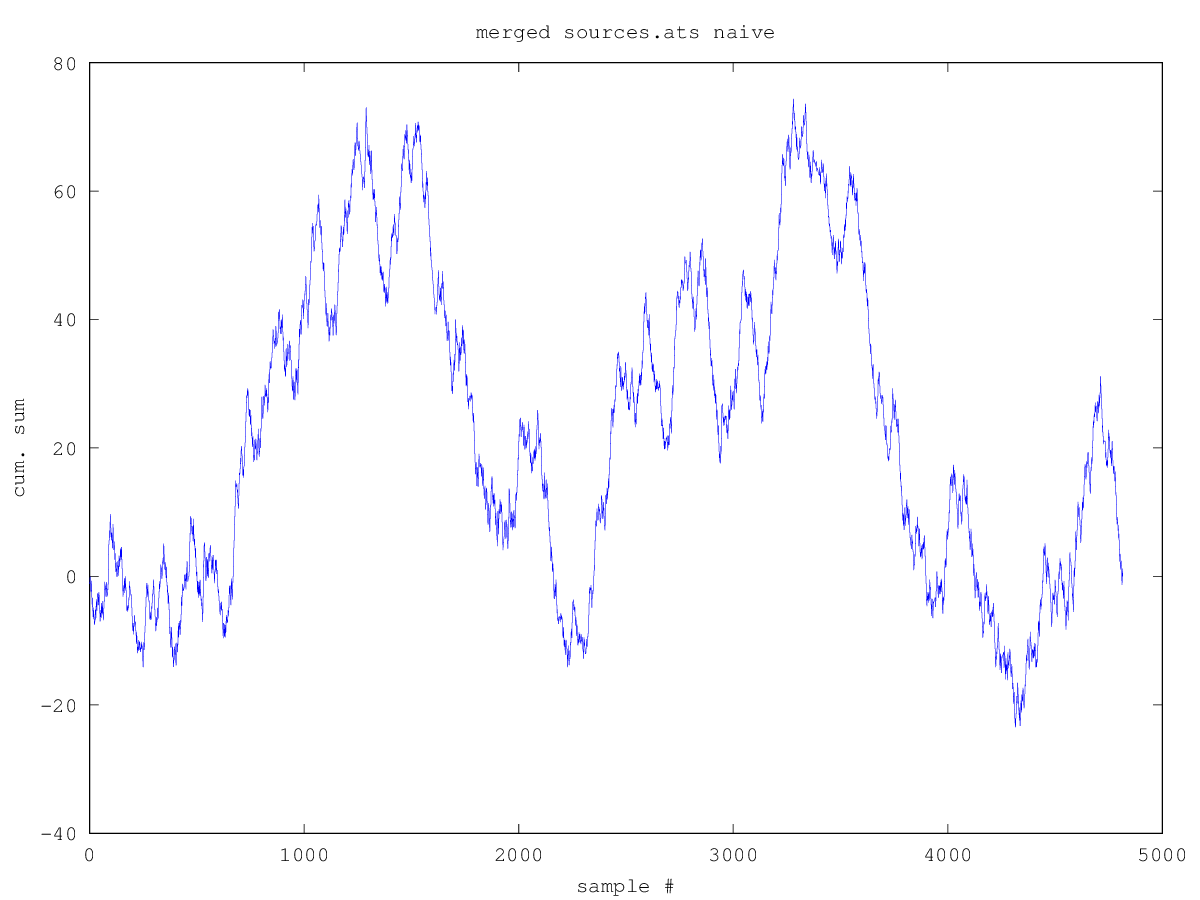
\includegraphics[width=0.8\linewidth]{{fractals/merged_data/merged_sources_ats_naive_time_series}.png}
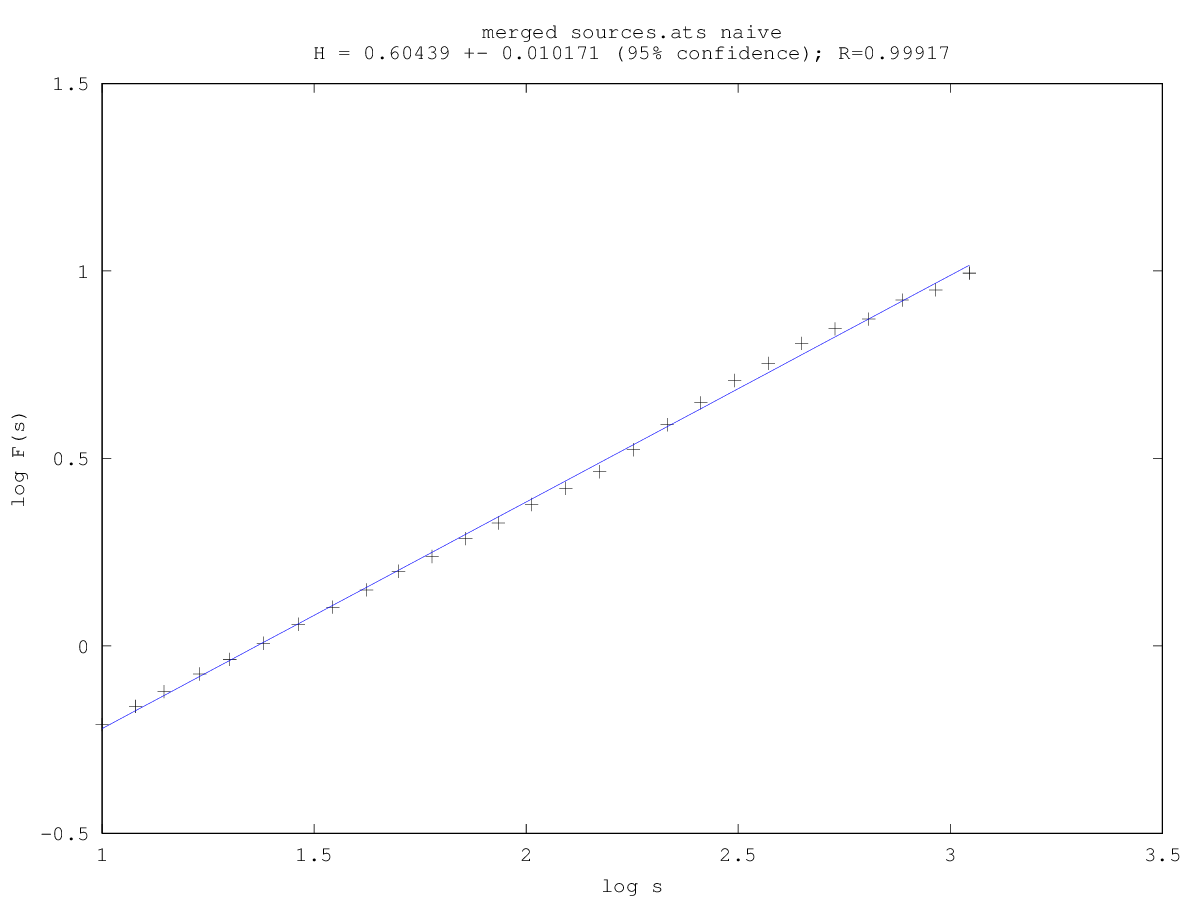
\includegraphics[width=0.8\linewidth]{{fractals/merged_data/merged_sources_ats_naive_log_log}.png}
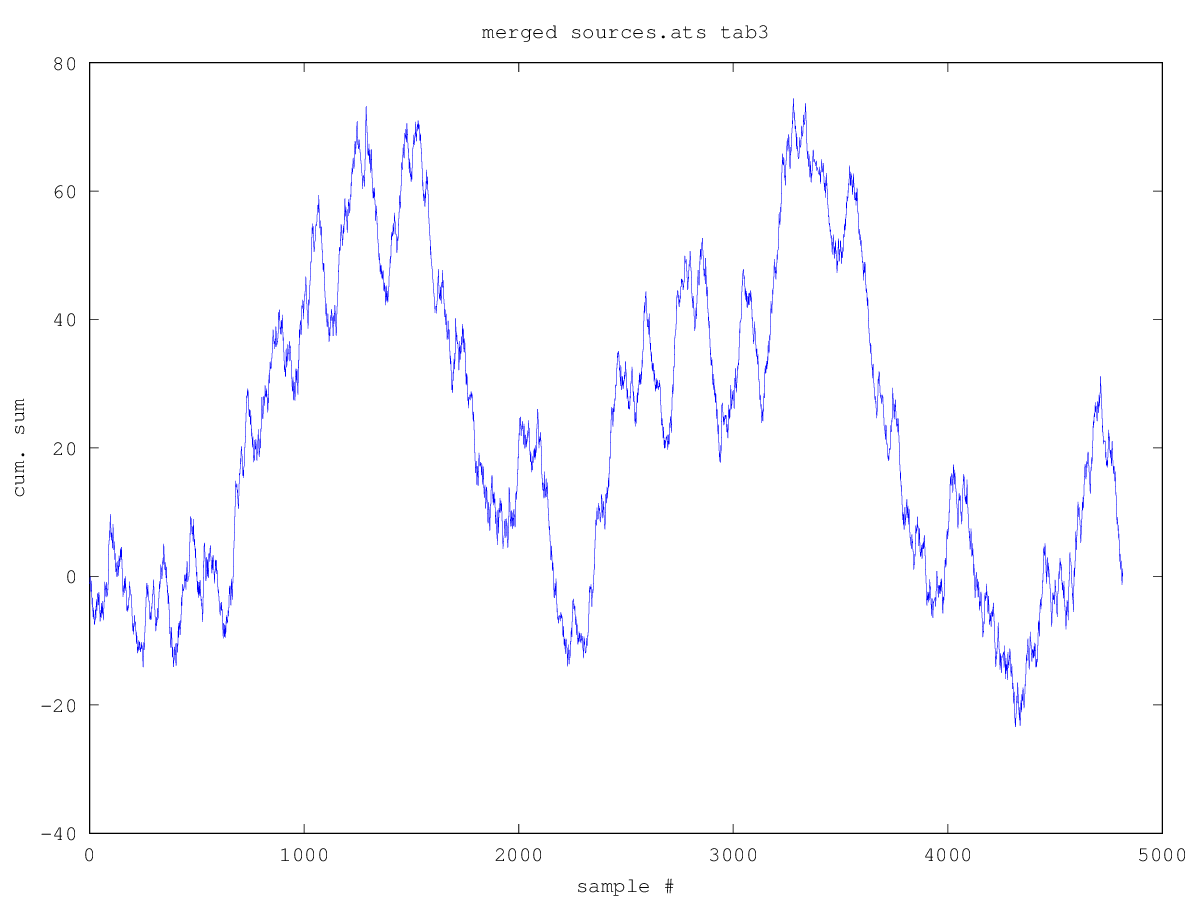
\includegraphics[width=0.8\linewidth]{{fractals/merged_data/merged_sources_ats_tab3_time_series}.png}
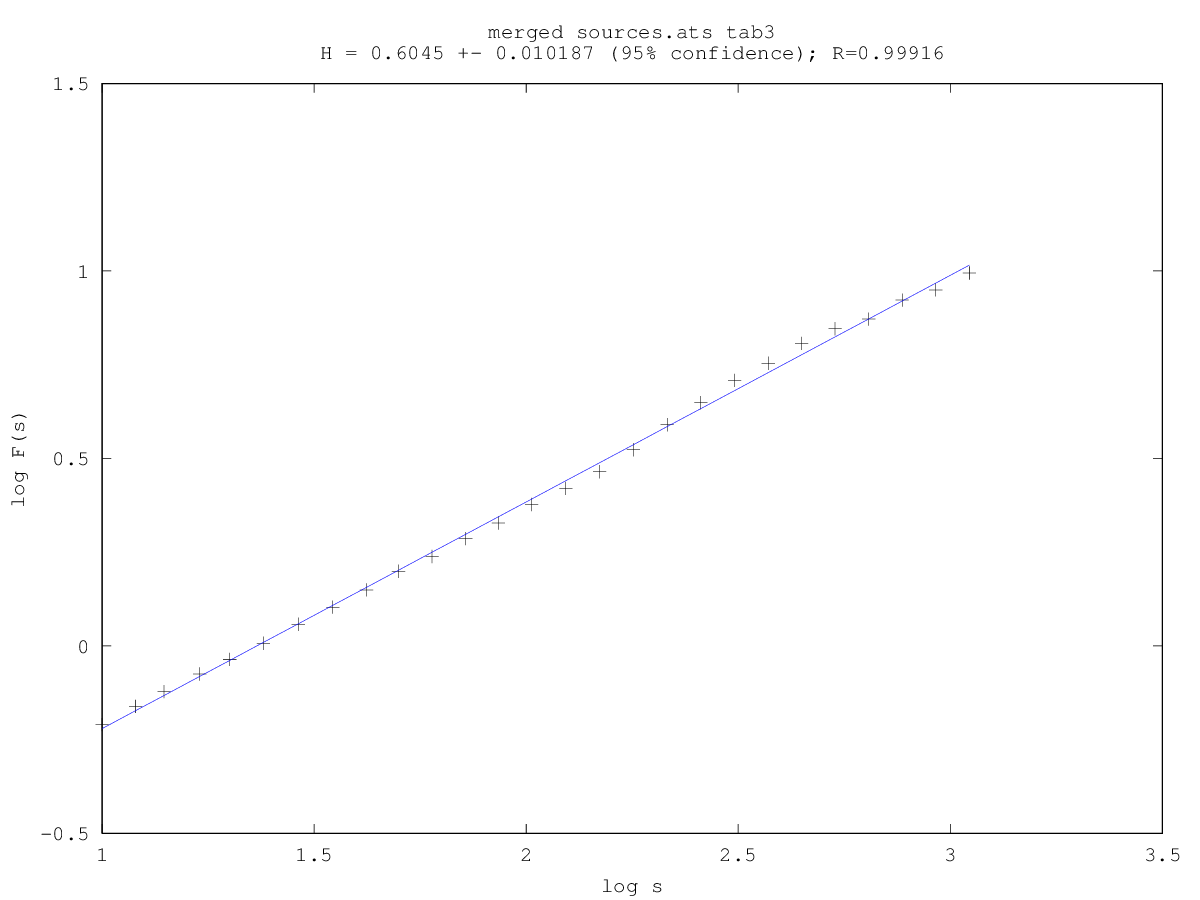
\includegraphics[width=0.8\linewidth]{{fractals/merged_data/merged_sources_ats_tab3_log_log}.png}
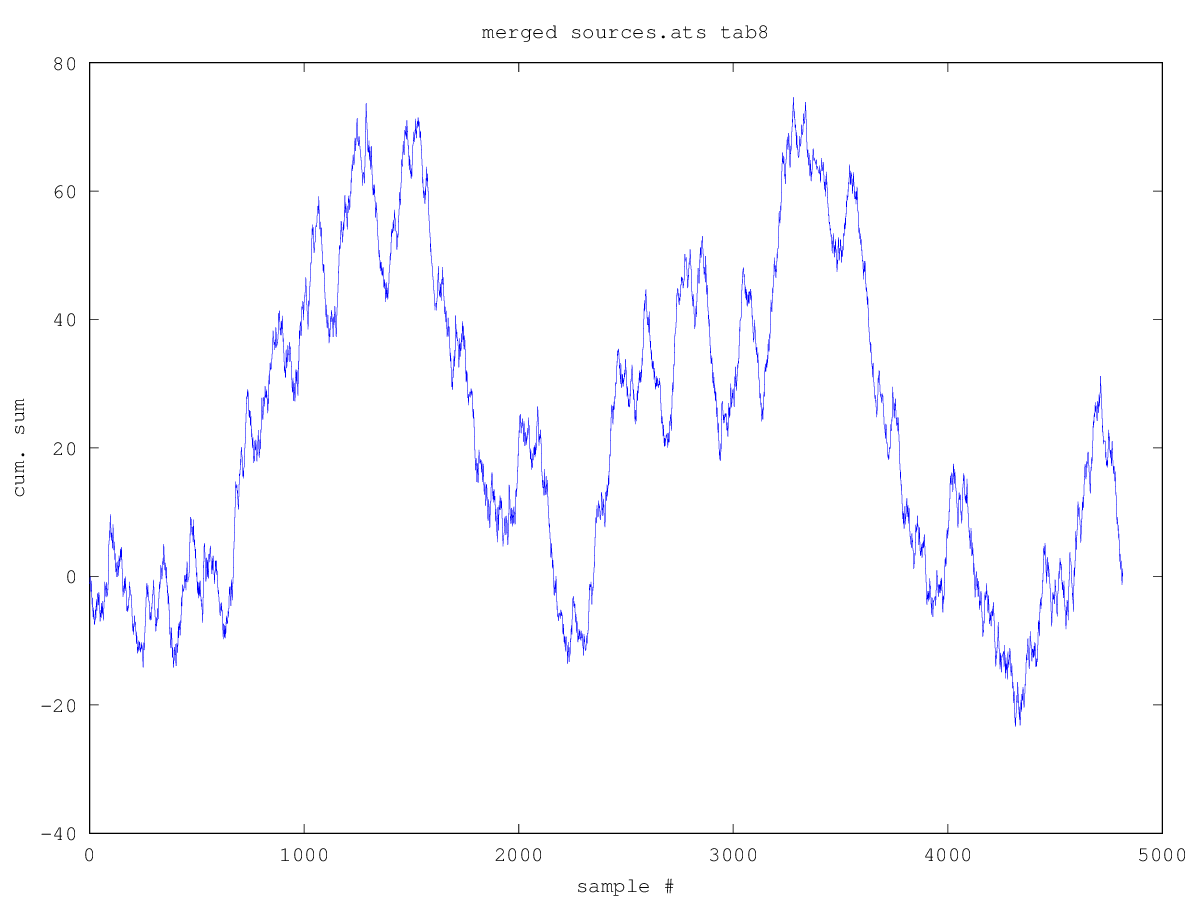
\includegraphics[width=0.8\linewidth]{{fractals/merged_data/merged_sources_ats_tab8_time_series}.png}
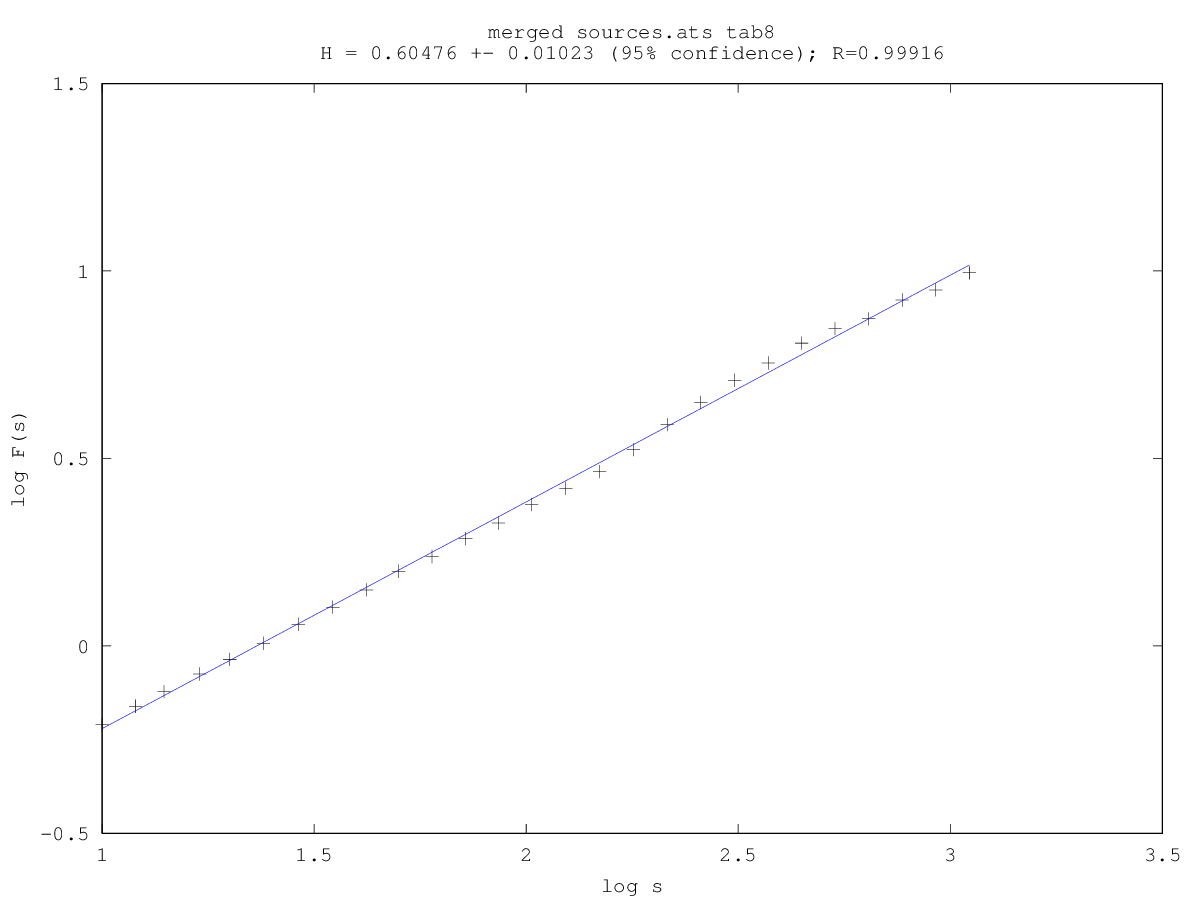
\includegraphics[width=0.8\linewidth]{{fractals/merged_data/merged_sources_ats_tab8_log_log}.png}
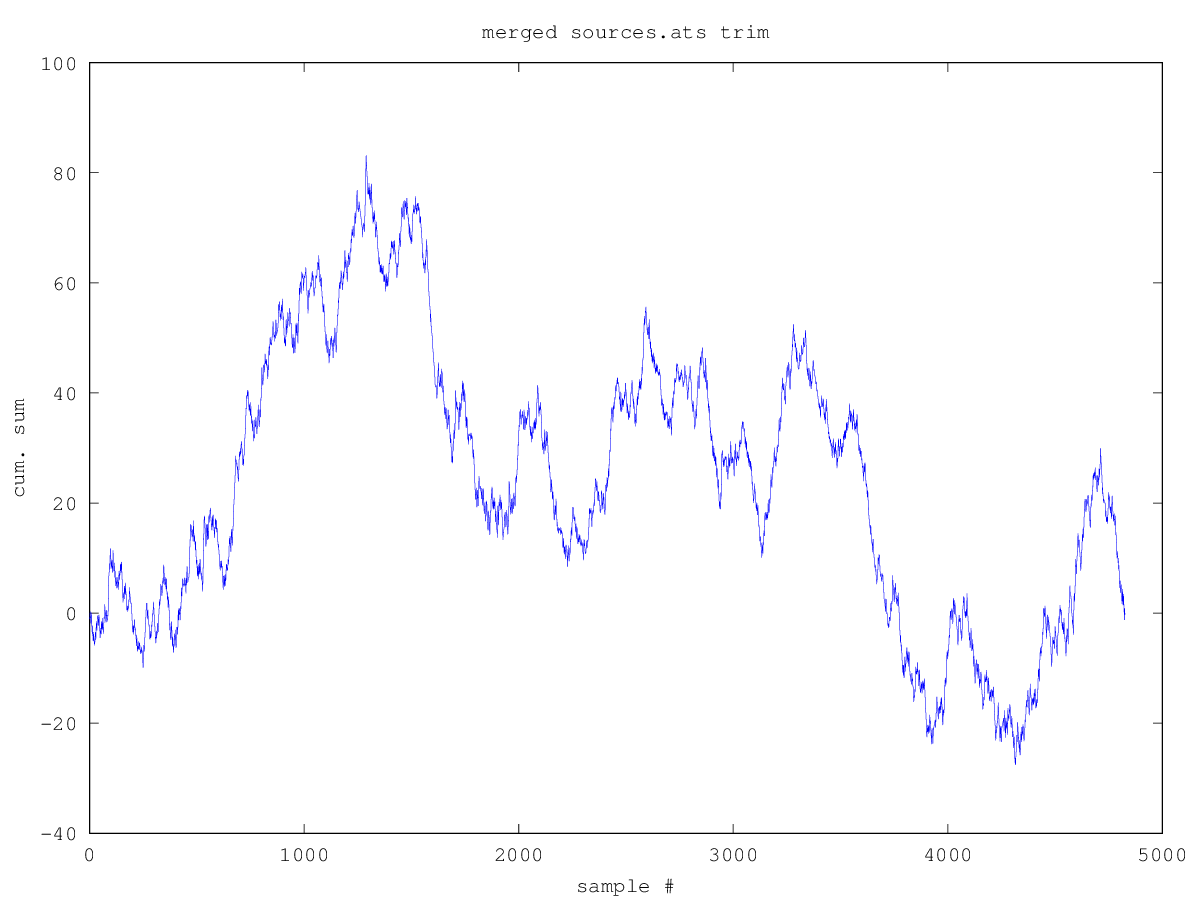
\includegraphics[width=0.8\linewidth]{{fractals/merged_data/merged_sources_ats_trim_time_series}.png}
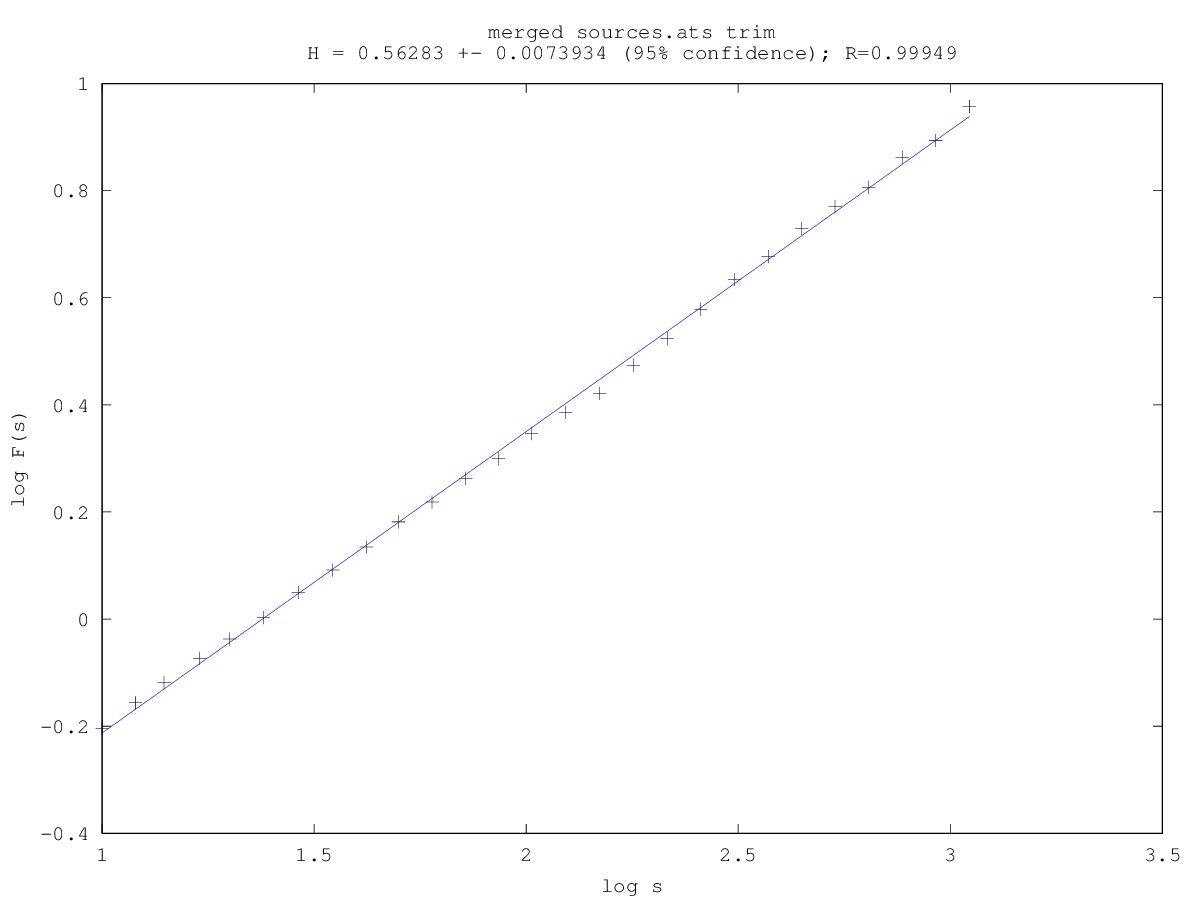
\includegraphics[width=0.8\linewidth]{{fractals/merged_data/merged_sources_ats_trim_log_log}.png}
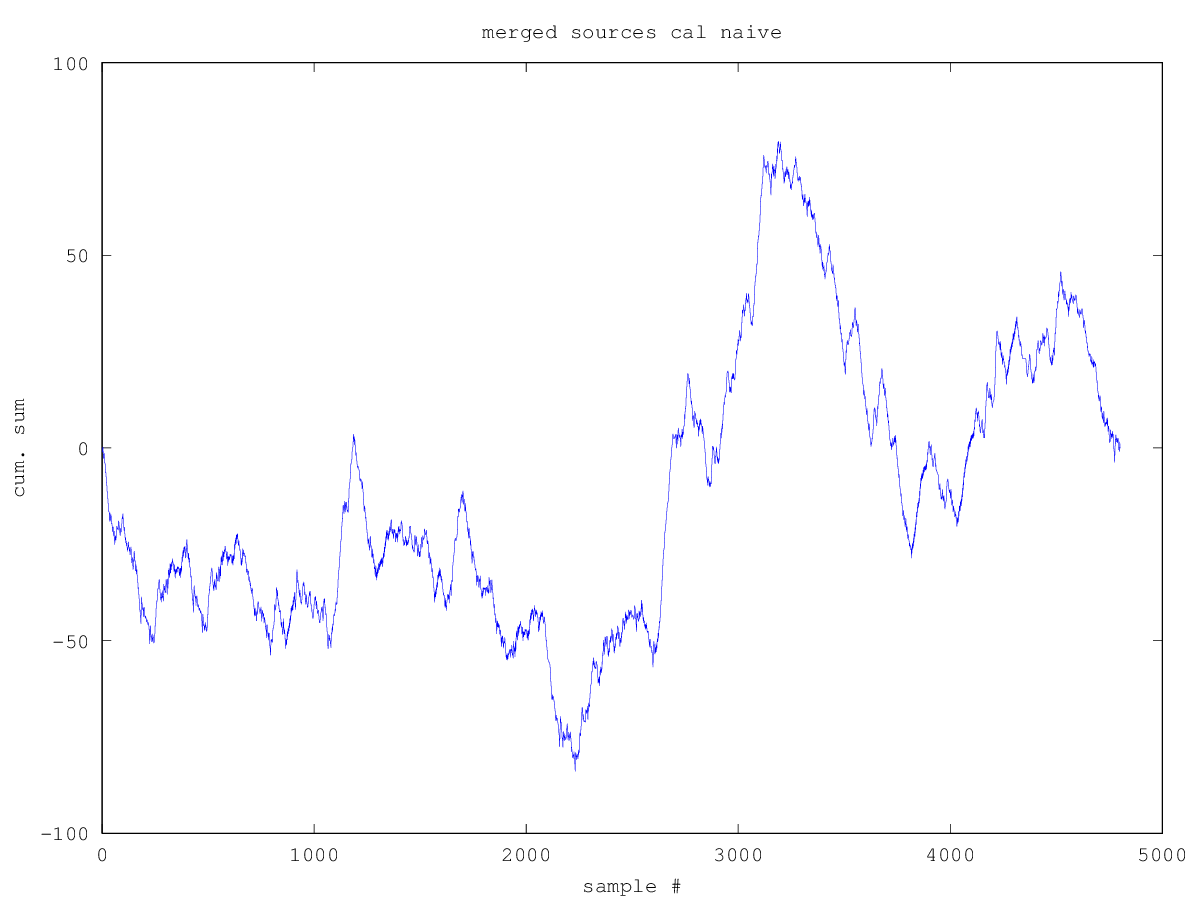
\includegraphics[width=0.8\linewidth]{{fractals/merged_data/merged_sources_cal_naive_time_series}.png}
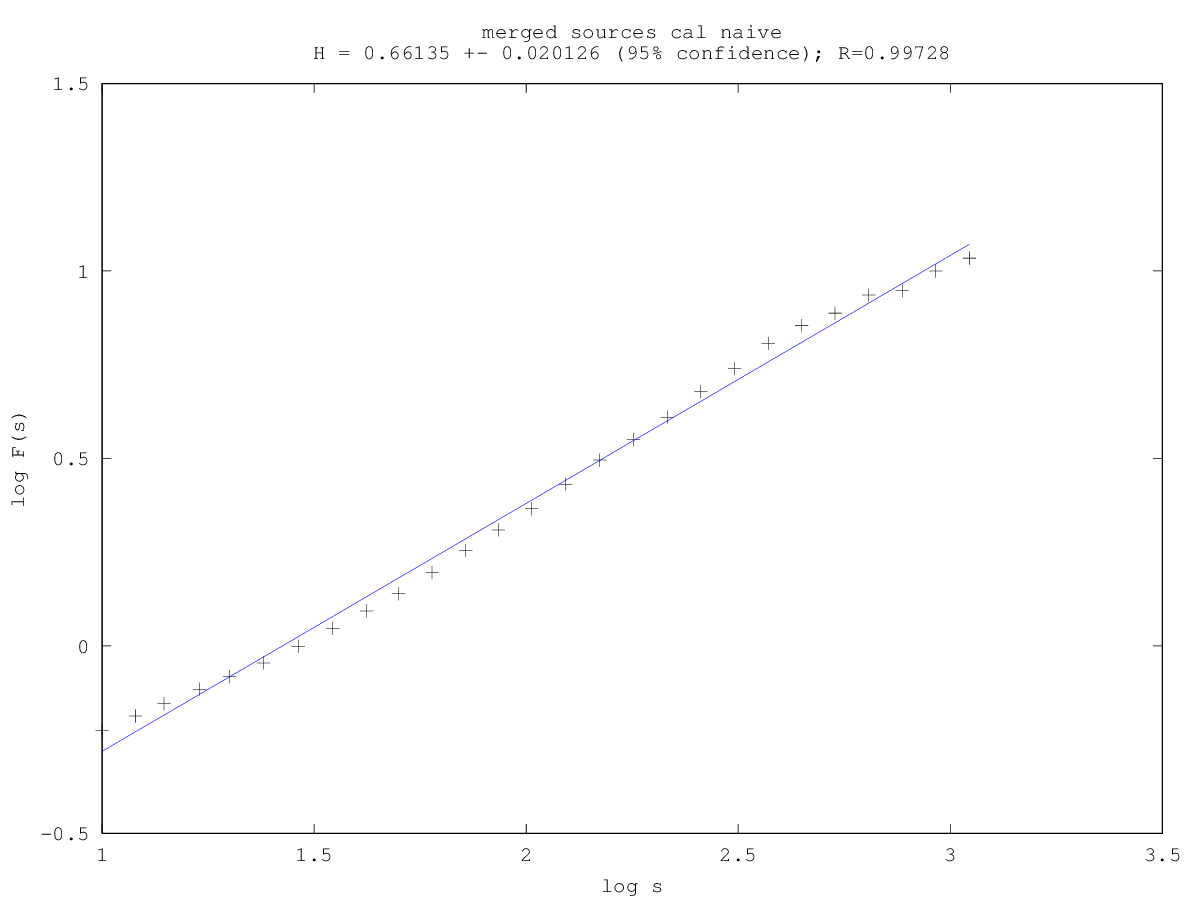
\includegraphics[width=0.8\linewidth]{{fractals/merged_data/merged_sources_cal_naive_log_log}.png}
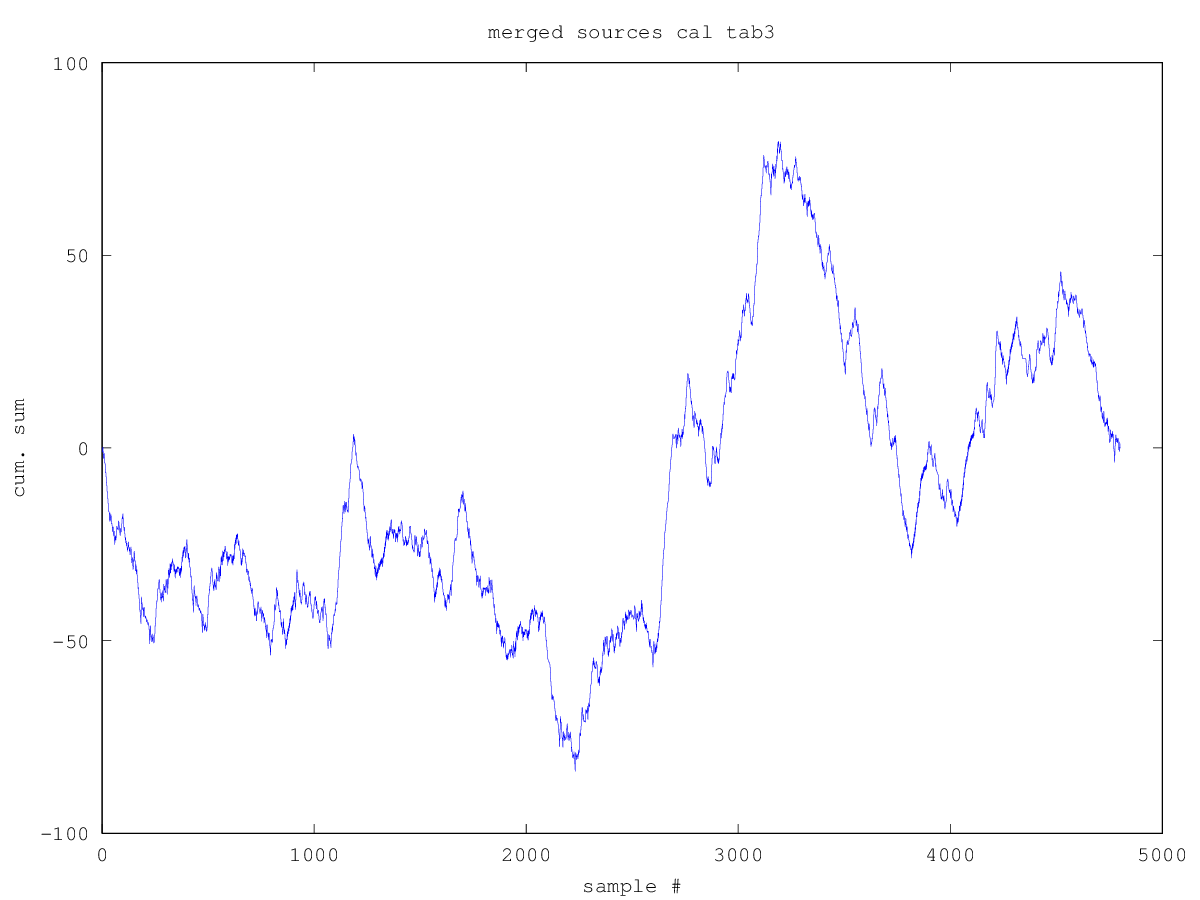
\includegraphics[width=0.8\linewidth]{{fractals/merged_data/merged_sources_cal_tab3_time_series}.png}
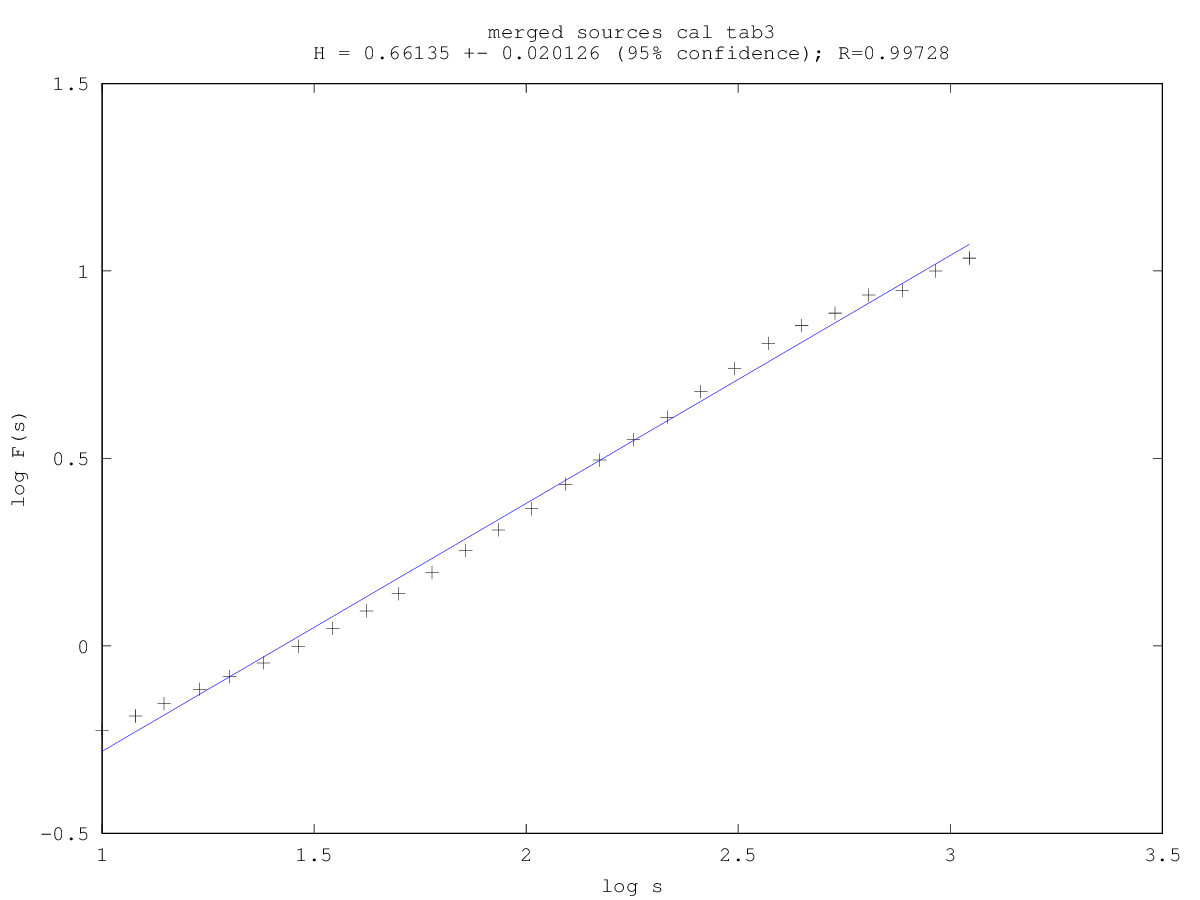
\includegraphics[width=0.8\linewidth]{{fractals/merged_data/merged_sources_cal_tab3_log_log}.png}
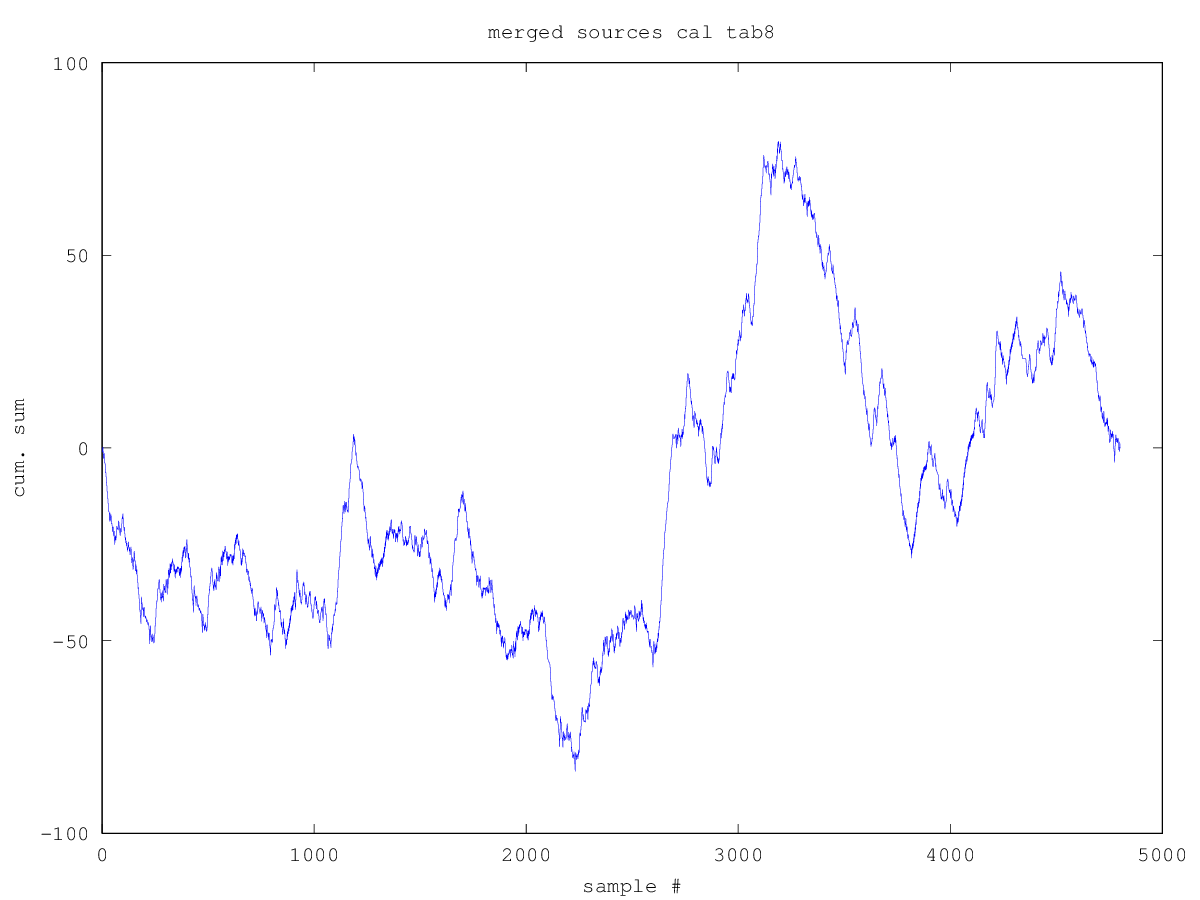
\includegraphics[width=0.8\linewidth]{{fractals/merged_data/merged_sources_cal_tab8_time_series}.png}
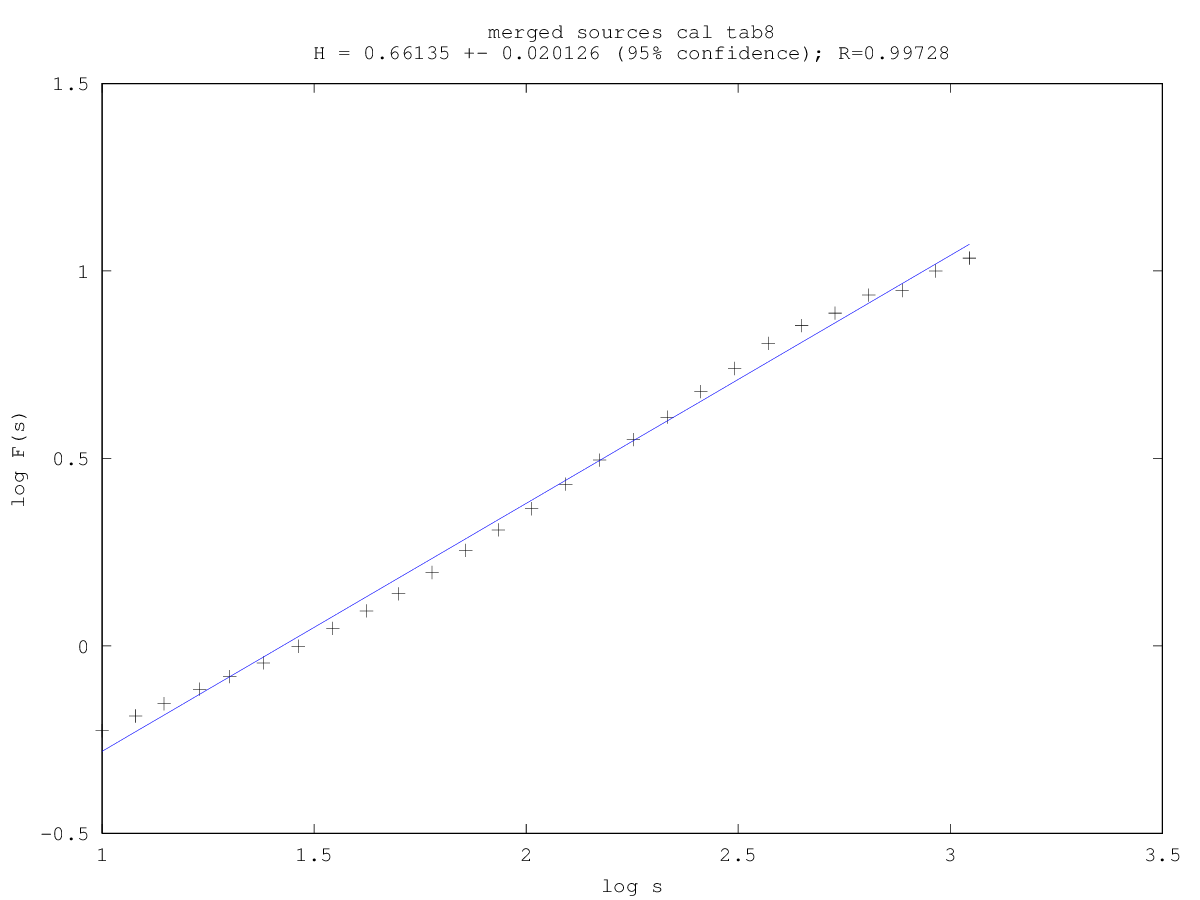
\includegraphics[width=0.8\linewidth]{{fractals/merged_data/merged_sources_cal_tab8_log_log}.png}
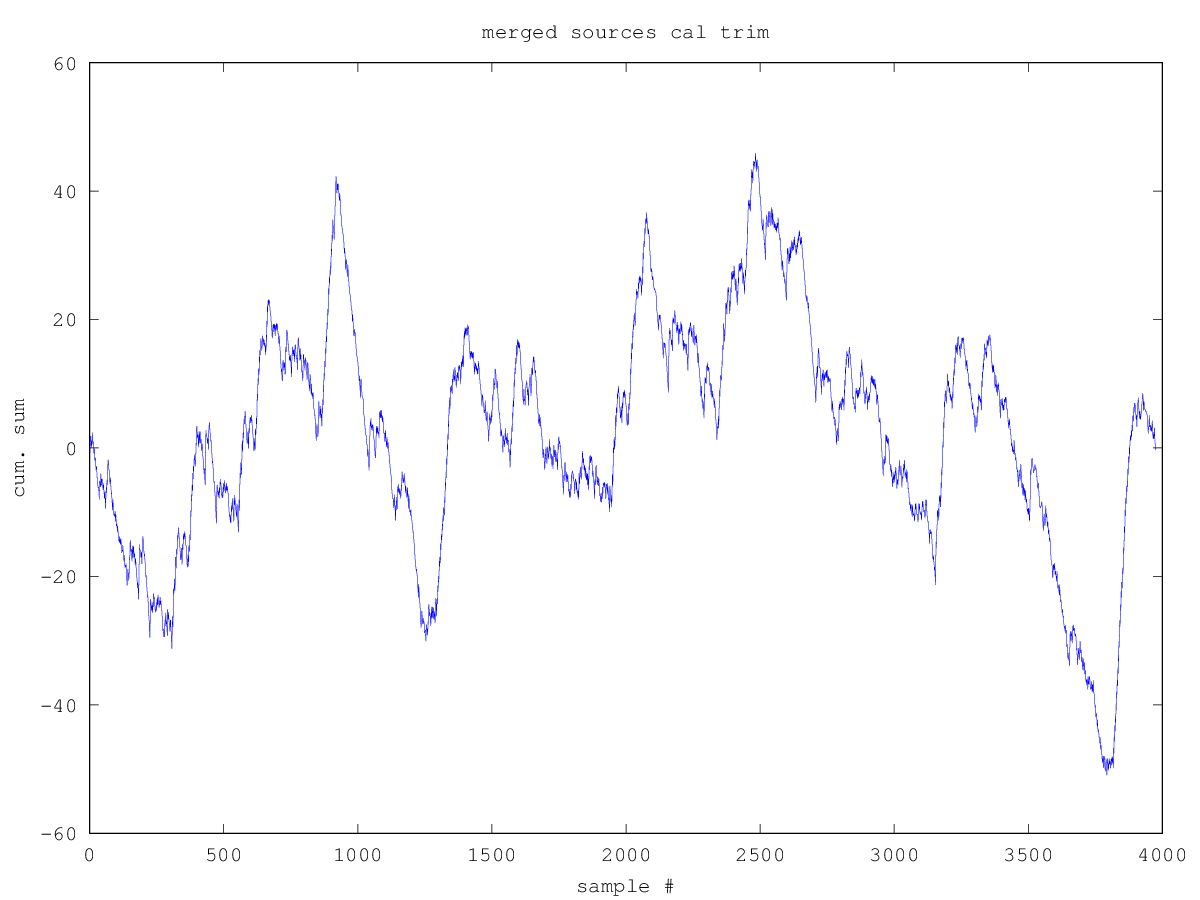
\includegraphics[width=0.8\linewidth]{{fractals/merged_data/merged_sources_cal_trim_time_series}.png}
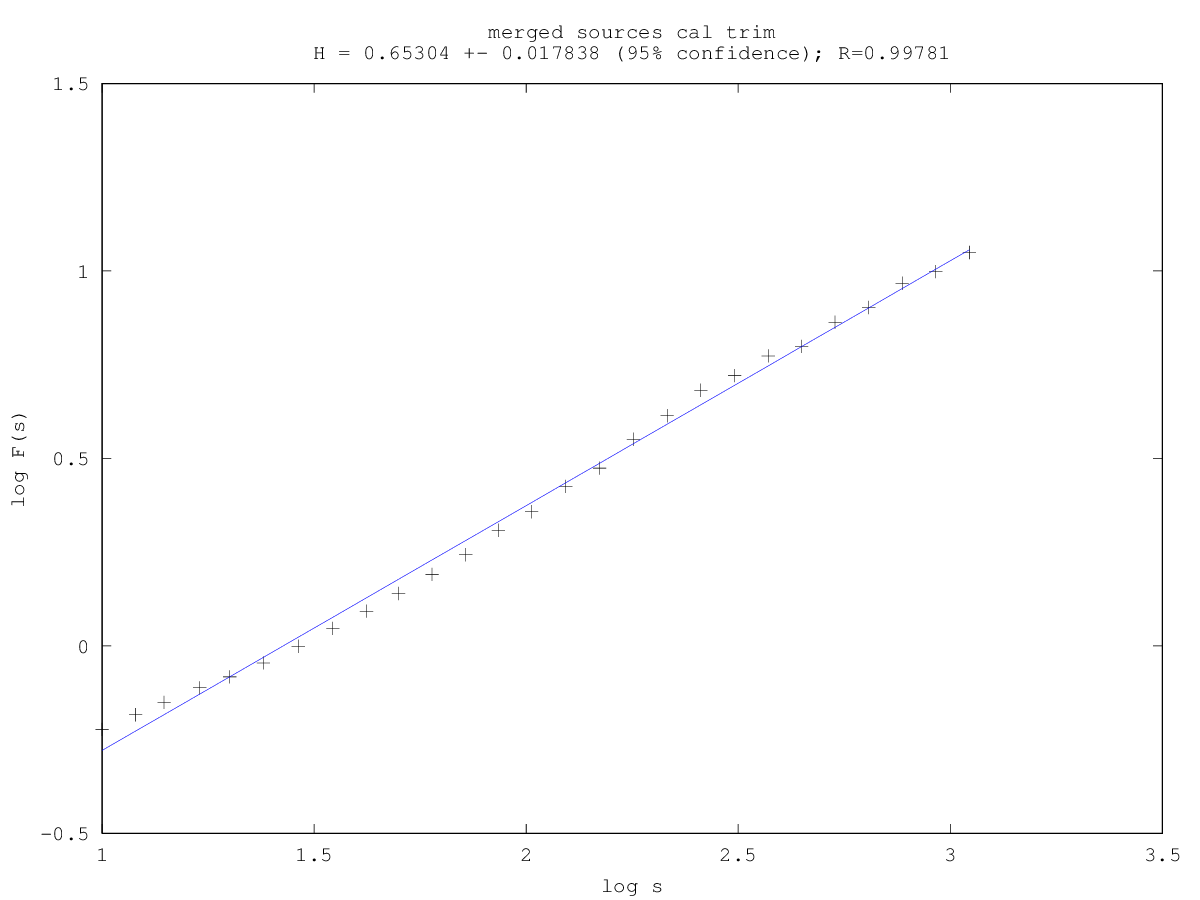
\includegraphics[width=0.8\linewidth]{{fractals/merged_data/merged_sources_cal_trim_log_log}.png}
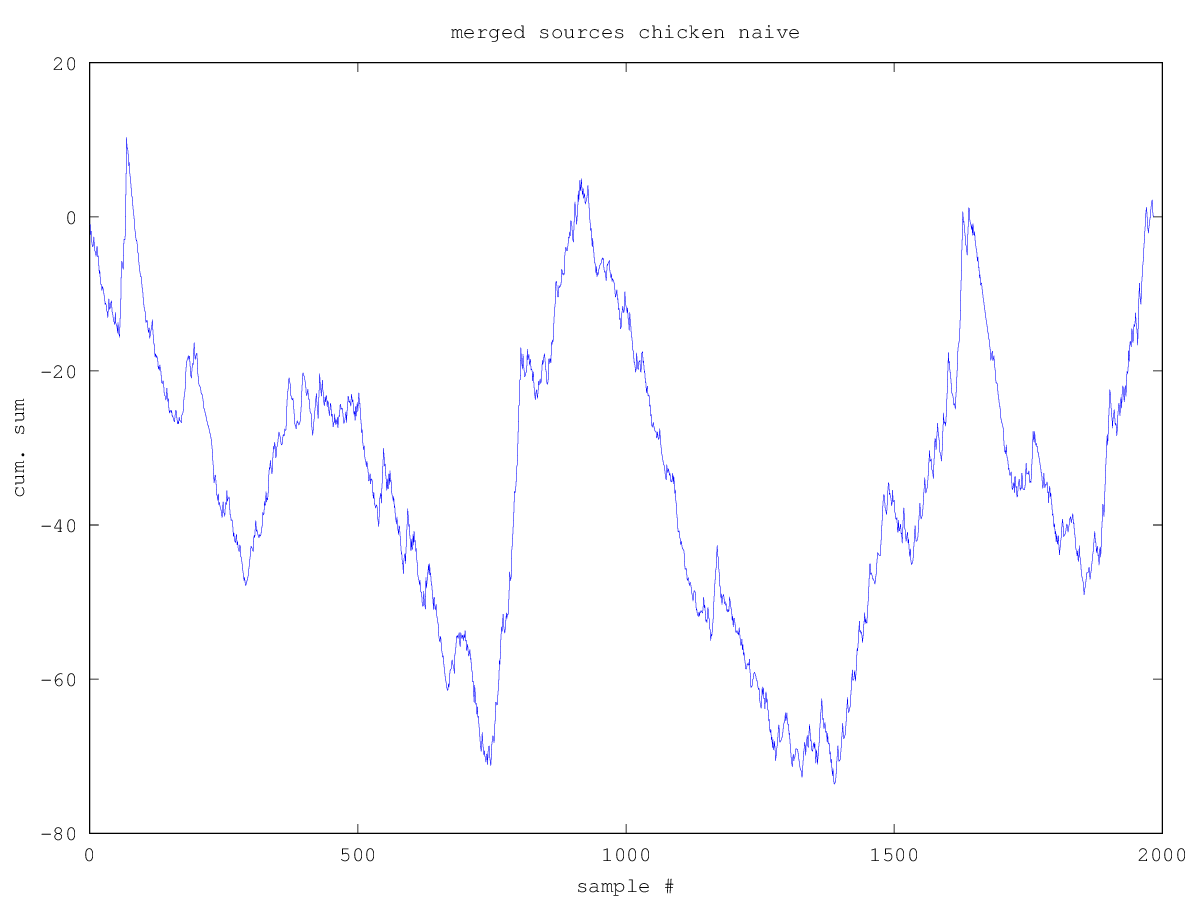
\includegraphics[width=0.8\linewidth]{{fractals/merged_data/merged_sources_chicken_naive_time_series}.png}
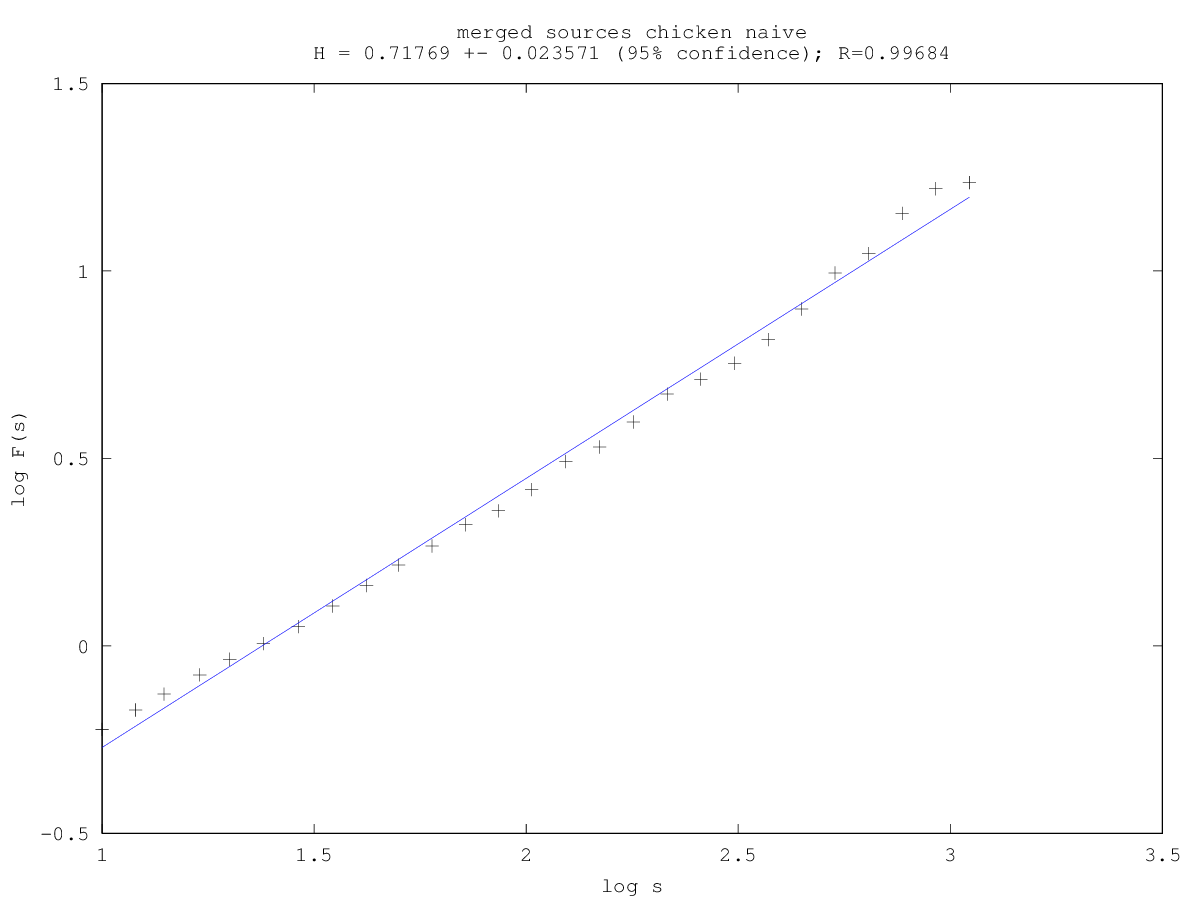
\includegraphics[width=0.8\linewidth]{{fractals/merged_data/merged_sources_chicken_naive_log_log}.png}
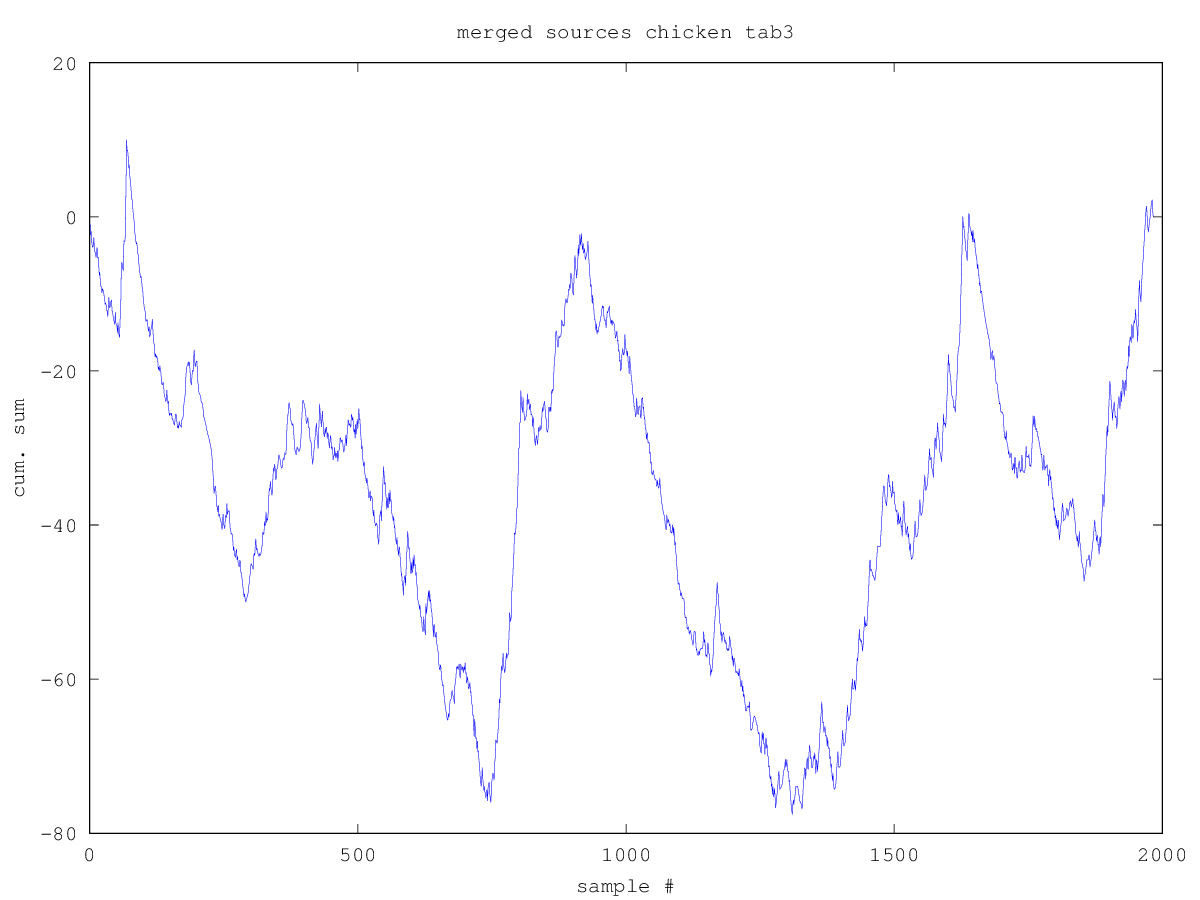
\includegraphics[width=0.8\linewidth]{{fractals/merged_data/merged_sources_chicken_tab3_time_series}.png}
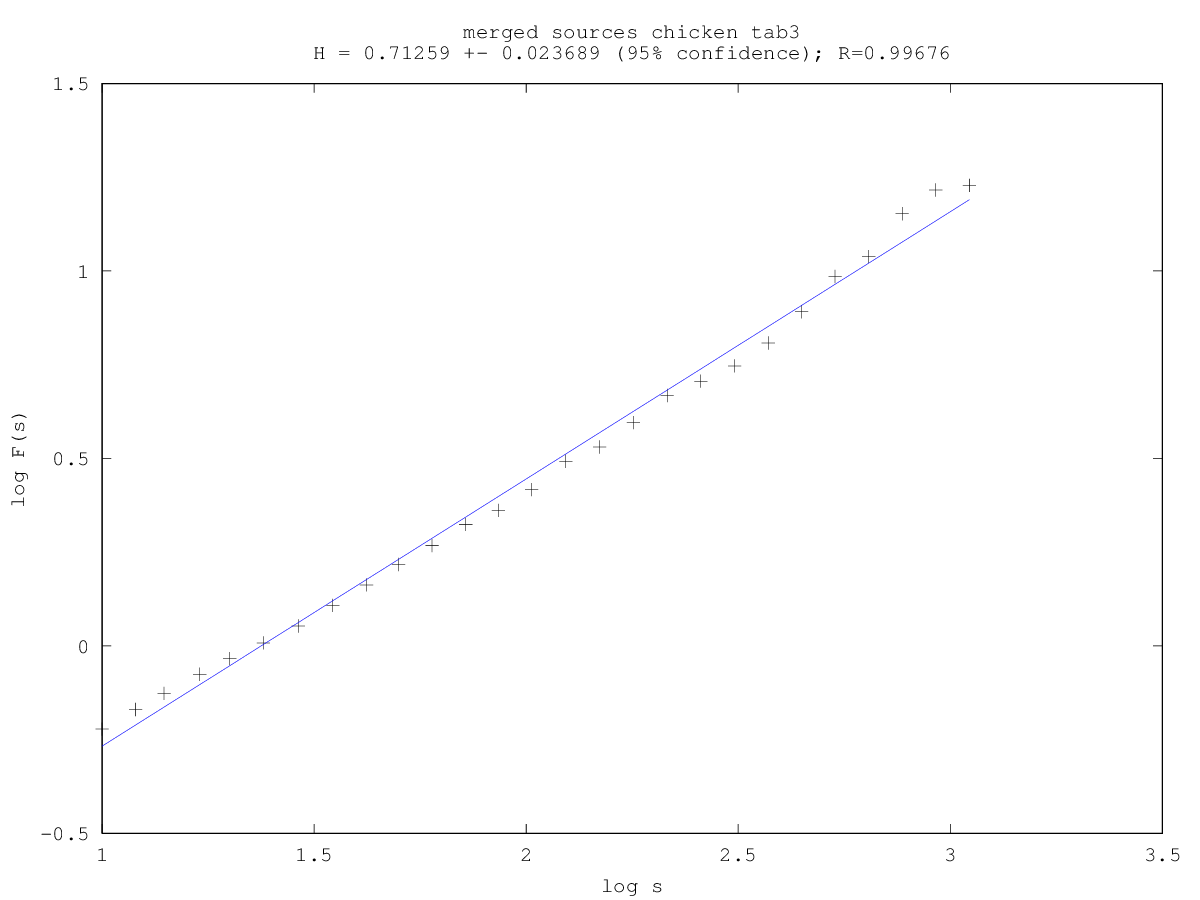
\includegraphics[width=0.8\linewidth]{{fractals/merged_data/merged_sources_chicken_tab3_log_log}.png}
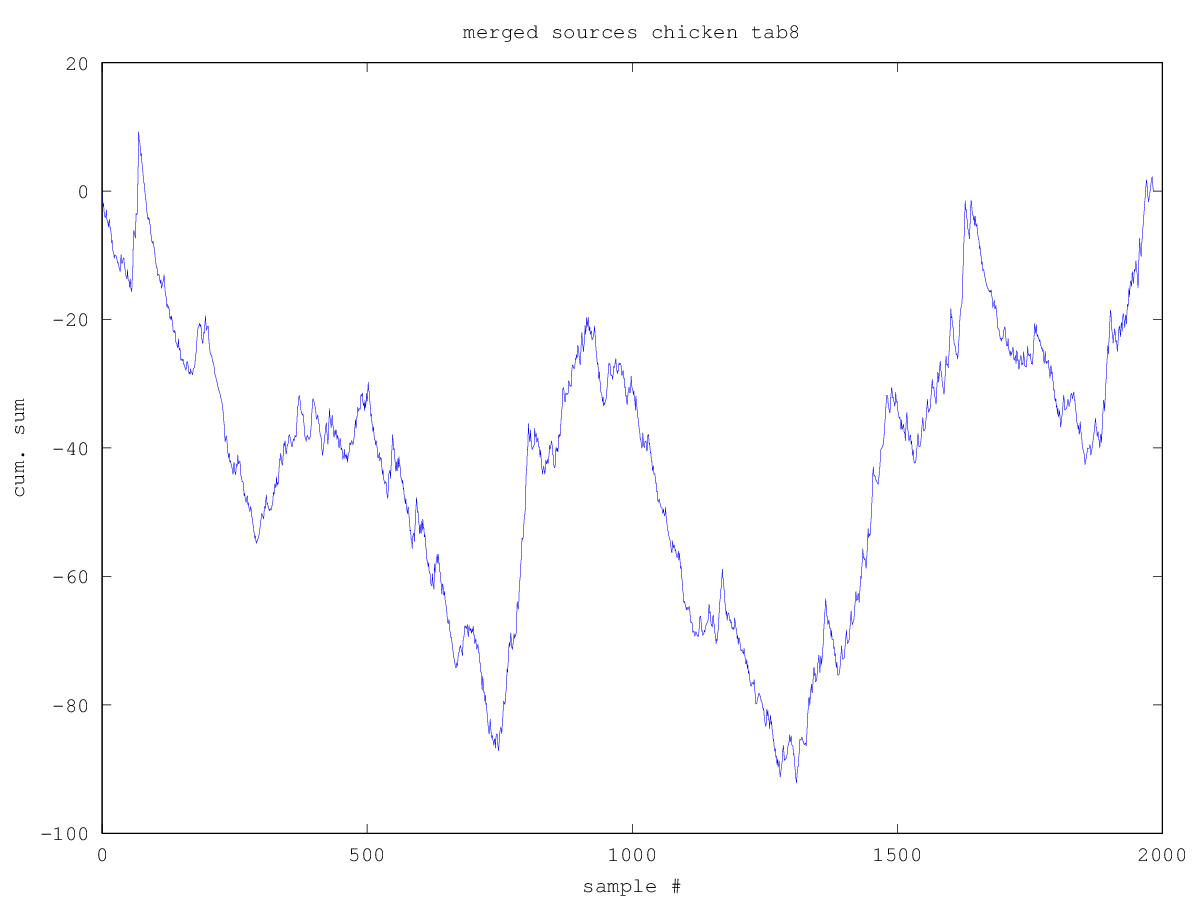
\includegraphics[width=0.8\linewidth]{{fractals/merged_data/merged_sources_chicken_tab8_time_series}.png}
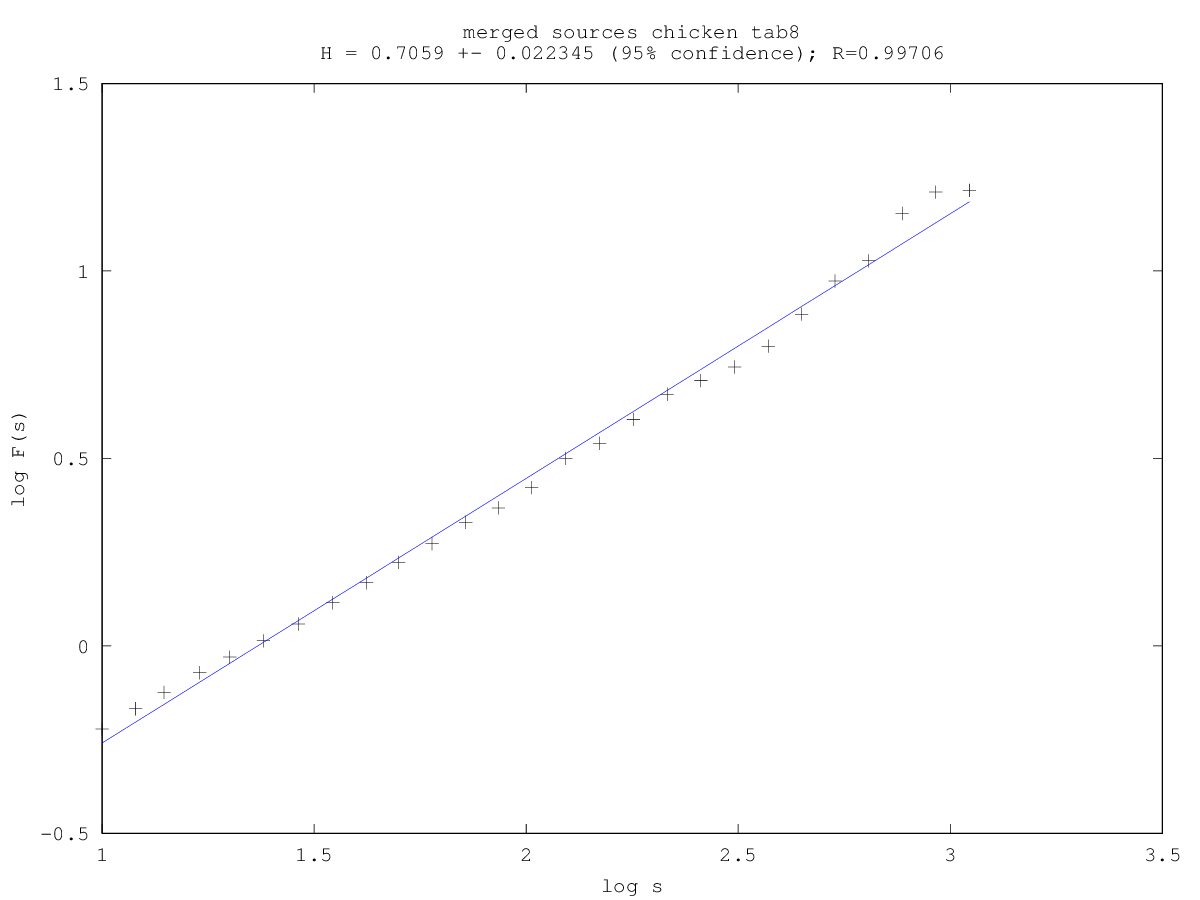
\includegraphics[width=0.8\linewidth]{{fractals/merged_data/merged_sources_chicken_tab8_log_log}.png}
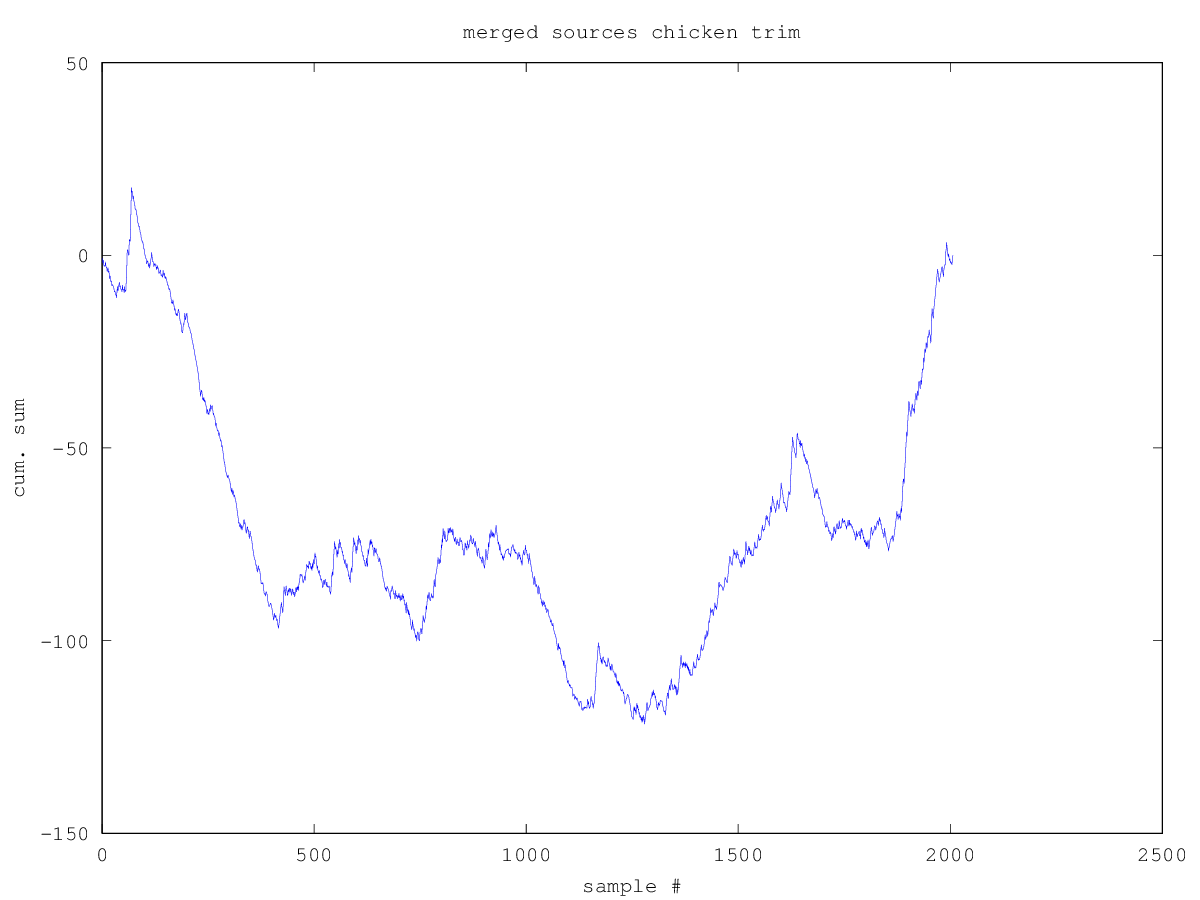
\includegraphics[width=0.8\linewidth]{{fractals/merged_data/merged_sources_chicken_trim_time_series}.png}
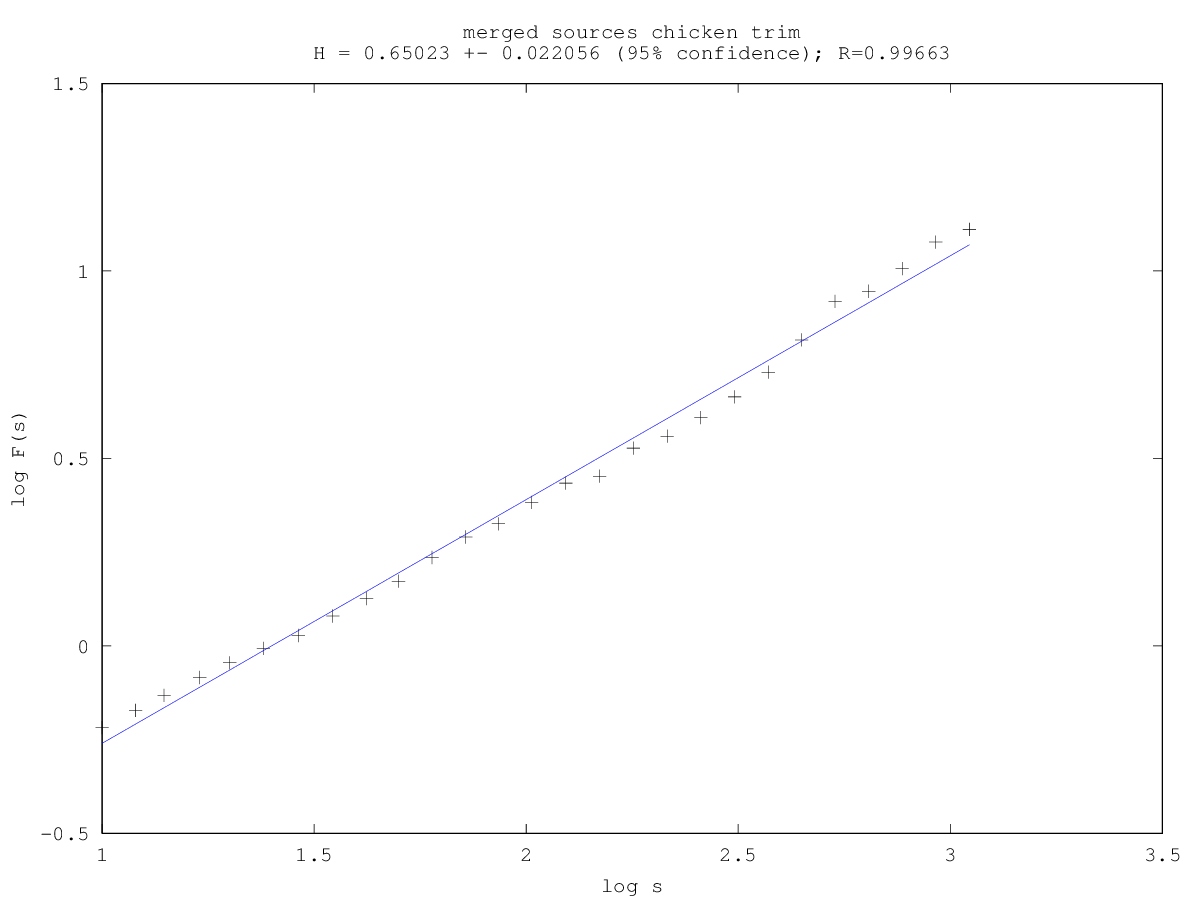
\includegraphics[width=0.8\linewidth]{{fractals/merged_data/merged_sources_chicken_trim_log_log}.png}
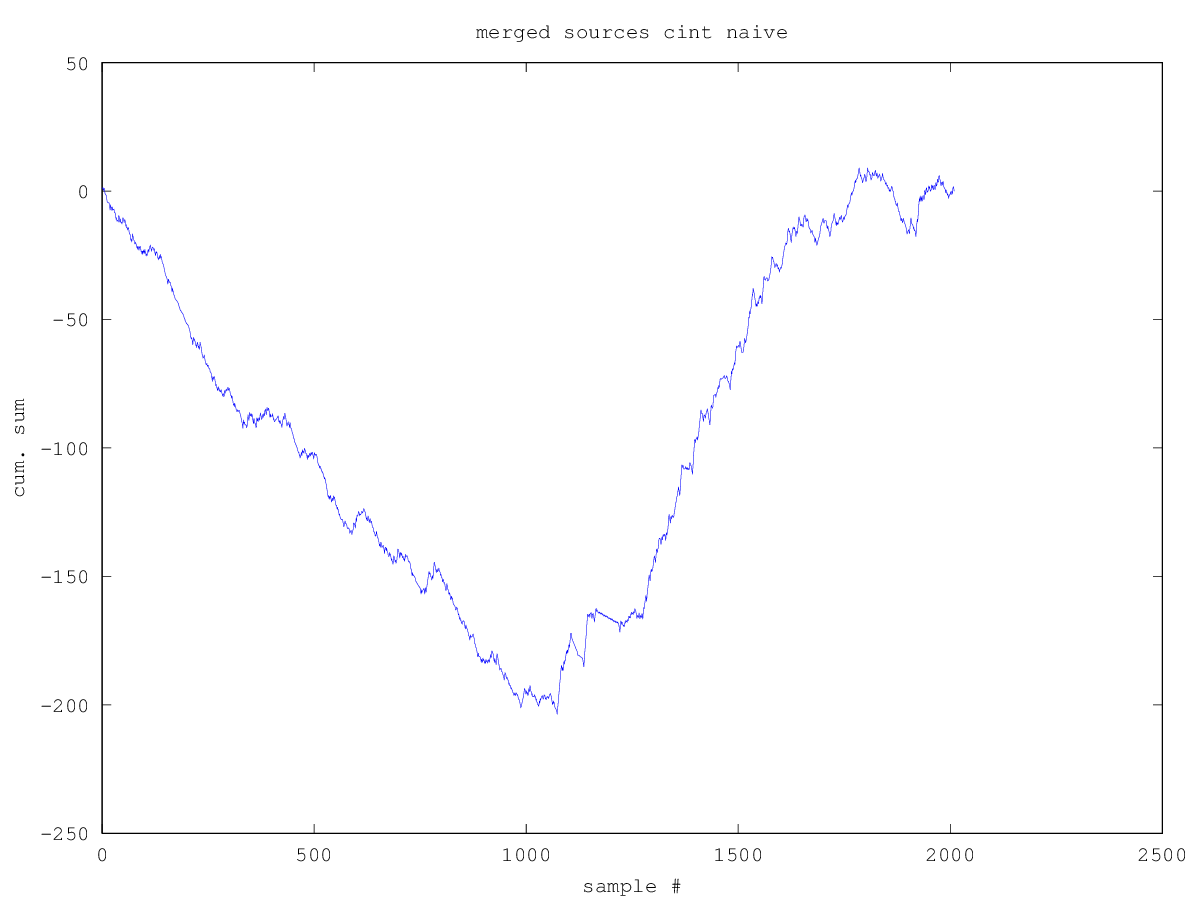
\includegraphics[width=0.8\linewidth]{{fractals/merged_data/merged_sources_cint_naive_time_series}.png}
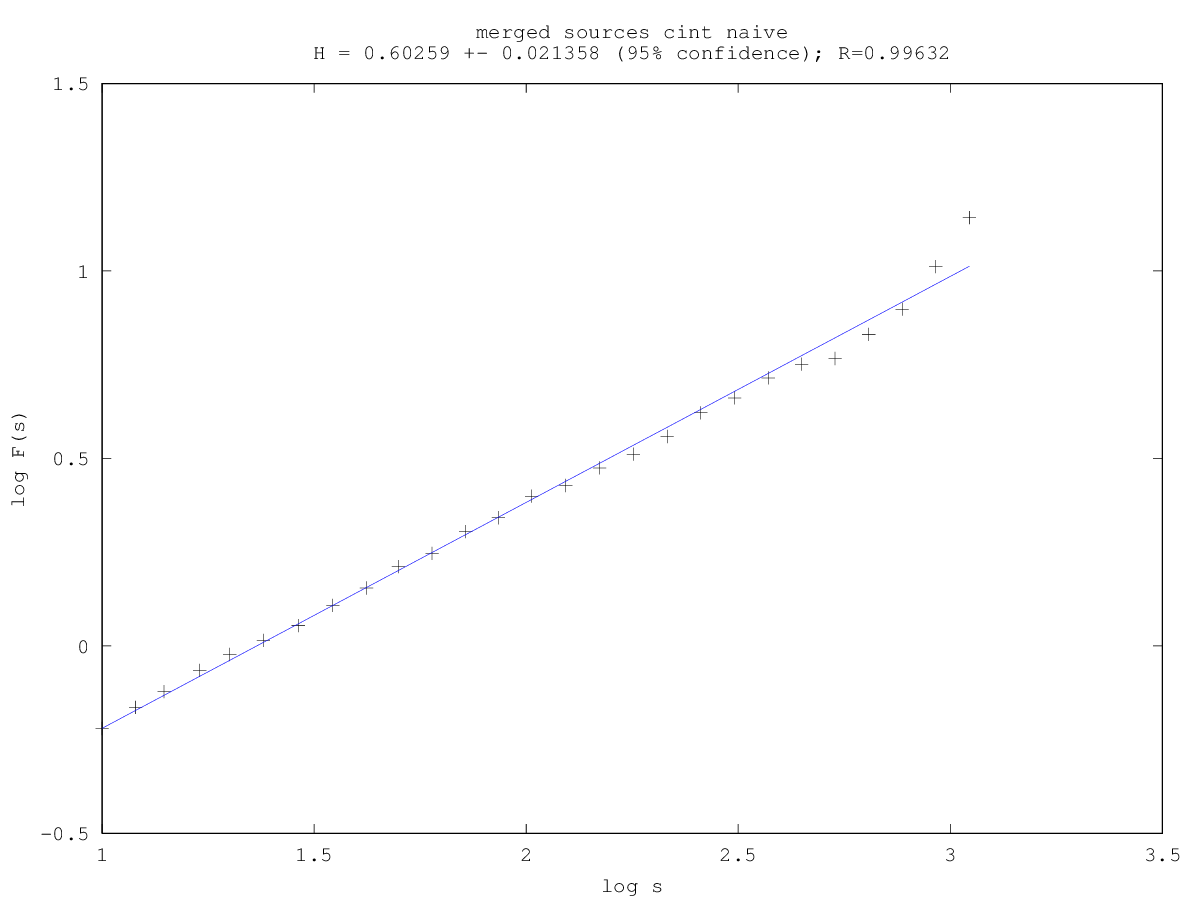
\includegraphics[width=0.8\linewidth]{{fractals/merged_data/merged_sources_cint_naive_log_log}.png}
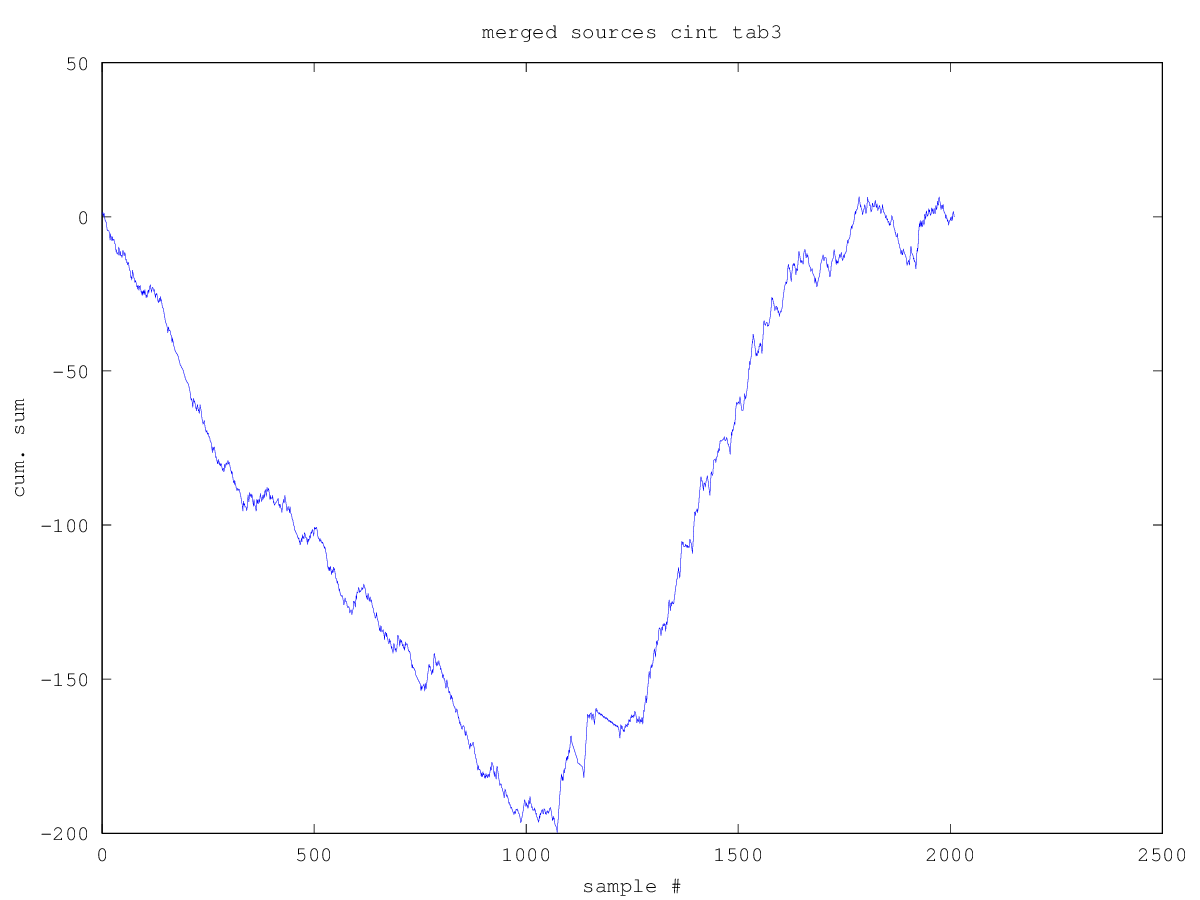
\includegraphics[width=0.8\linewidth]{{fractals/merged_data/merged_sources_cint_tab3_time_series}.png}
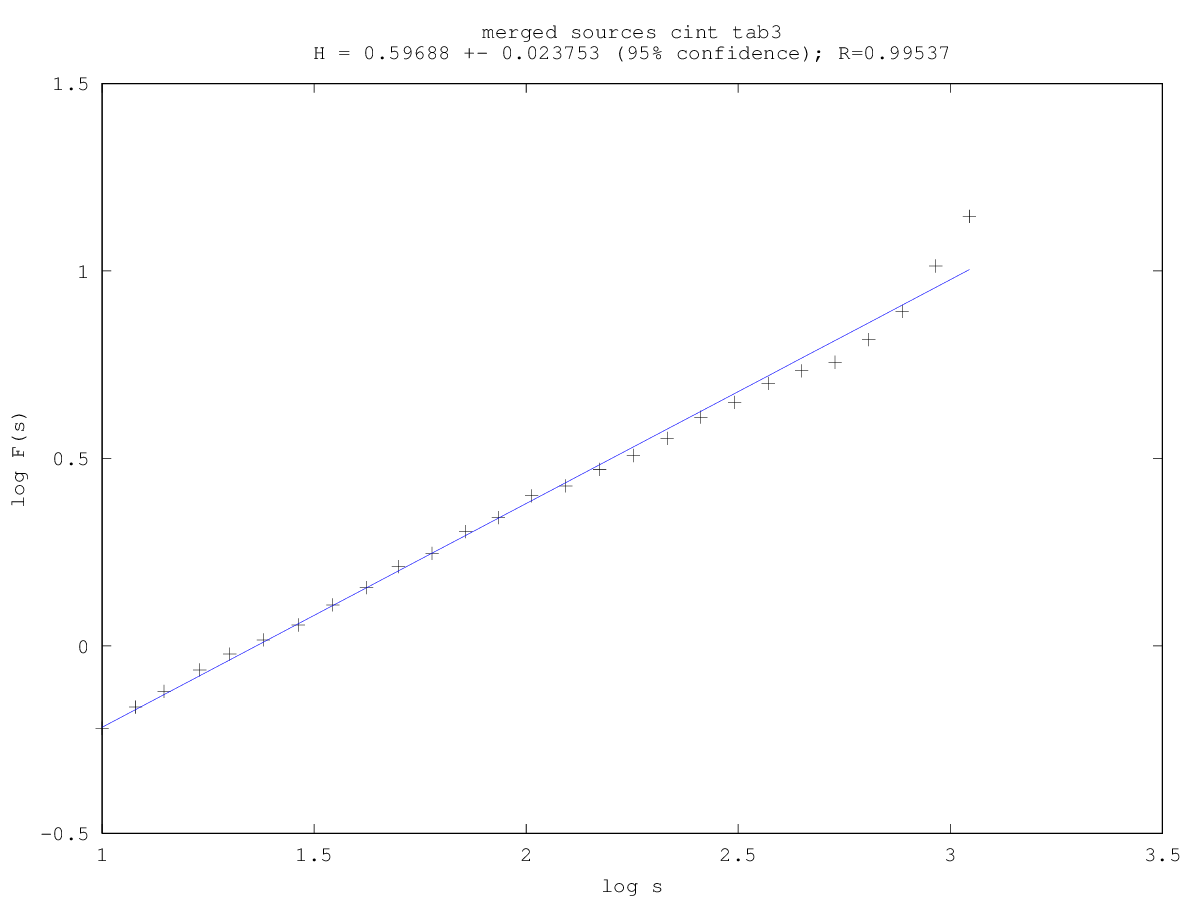
\includegraphics[width=0.8\linewidth]{{fractals/merged_data/merged_sources_cint_tab3_log_log}.png}
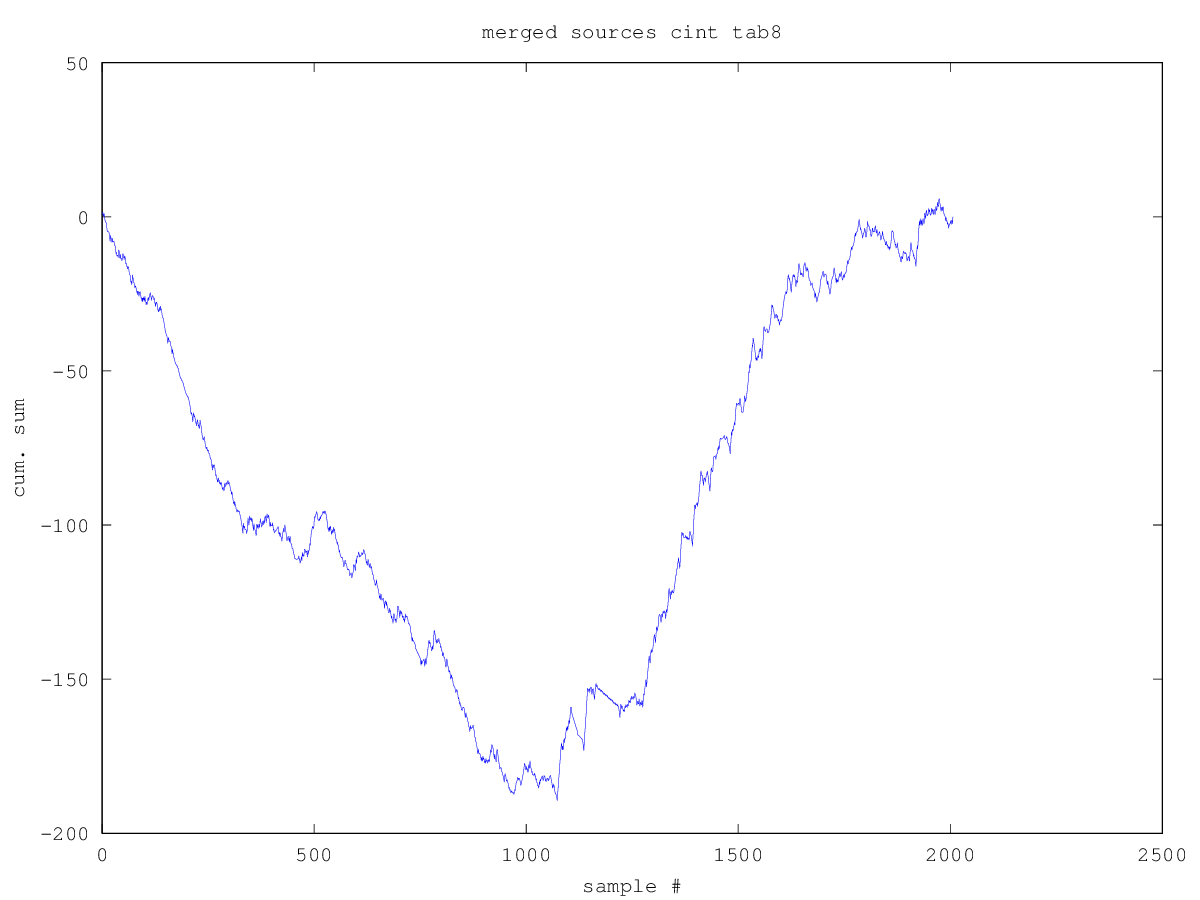
\includegraphics[width=0.8\linewidth]{{fractals/merged_data/merged_sources_cint_tab8_time_series}.png}
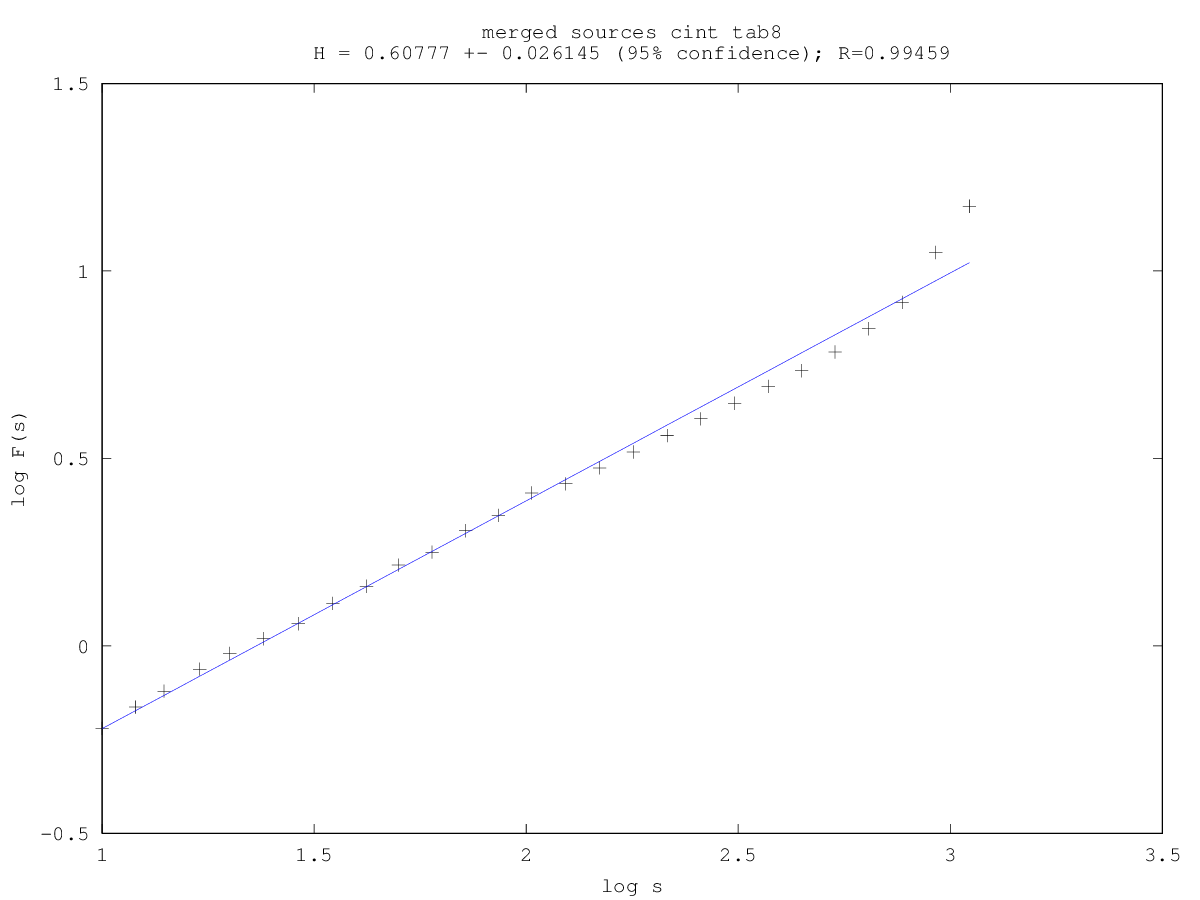
\includegraphics[width=0.8\linewidth]{{fractals/merged_data/merged_sources_cint_tab8_log_log}.png}
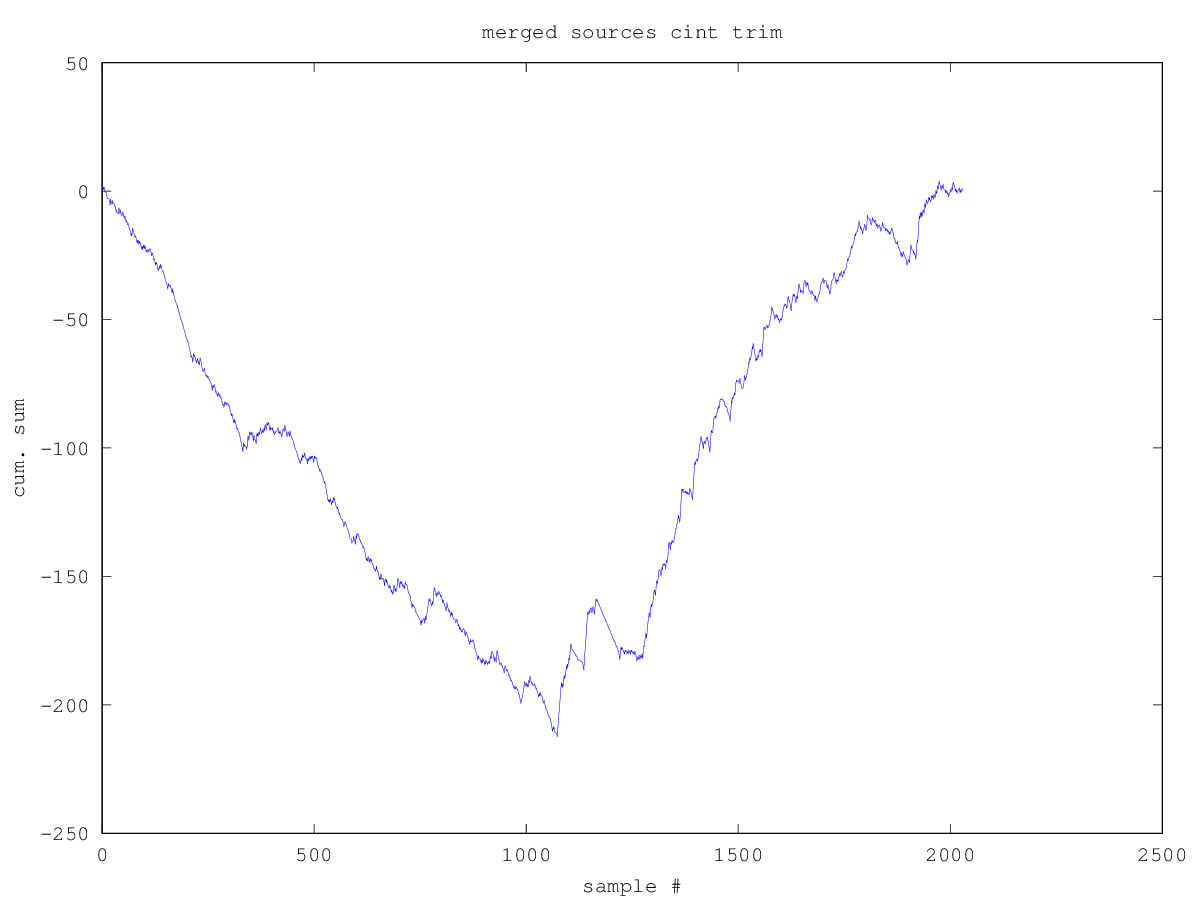
\includegraphics[width=0.8\linewidth]{{fractals/merged_data/merged_sources_cint_trim_time_series}.png}
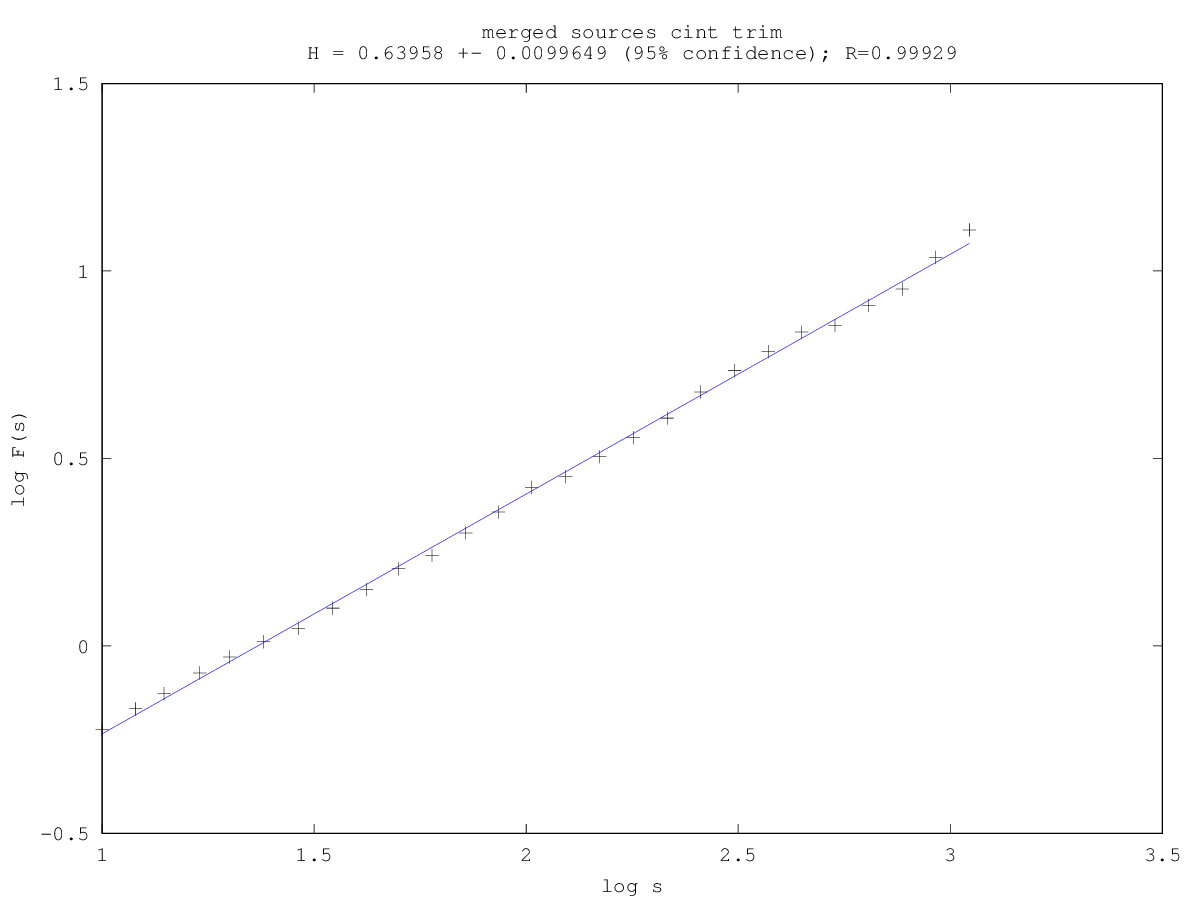
\includegraphics[width=0.8\linewidth]{{fractals/merged_data/merged_sources_cint_trim_log_log}.png}
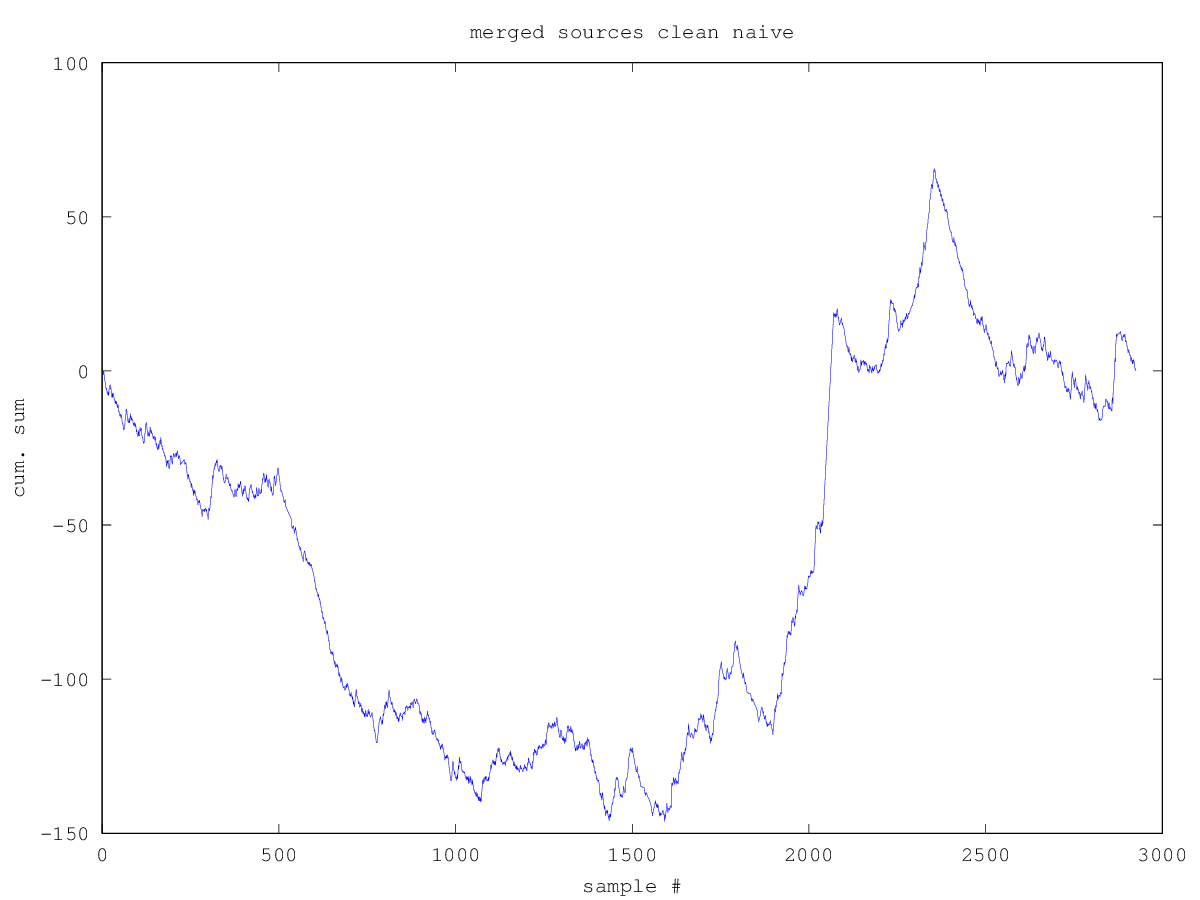
\includegraphics[width=0.8\linewidth]{{fractals/merged_data/merged_sources_clean_naive_time_series}.png}
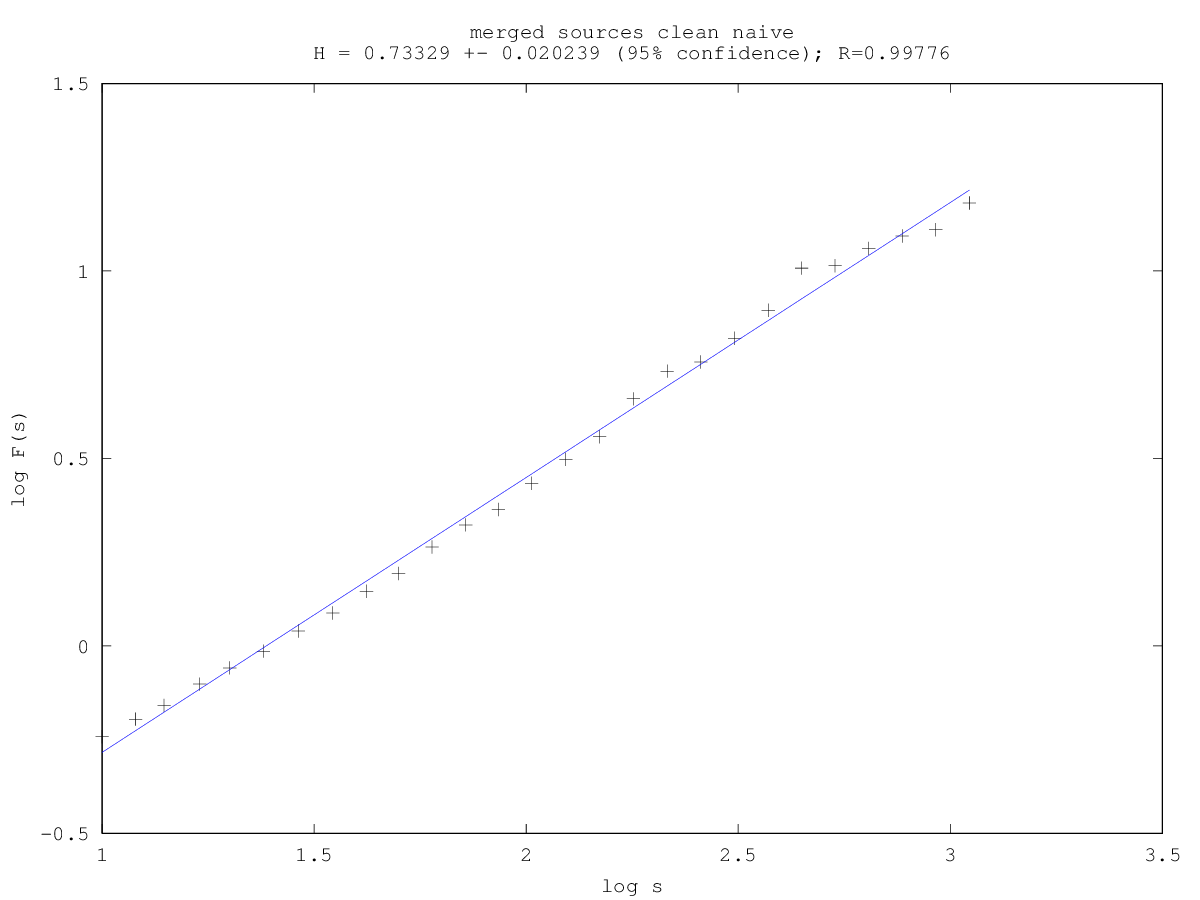
\includegraphics[width=0.8\linewidth]{{fractals/merged_data/merged_sources_clean_naive_log_log}.png}
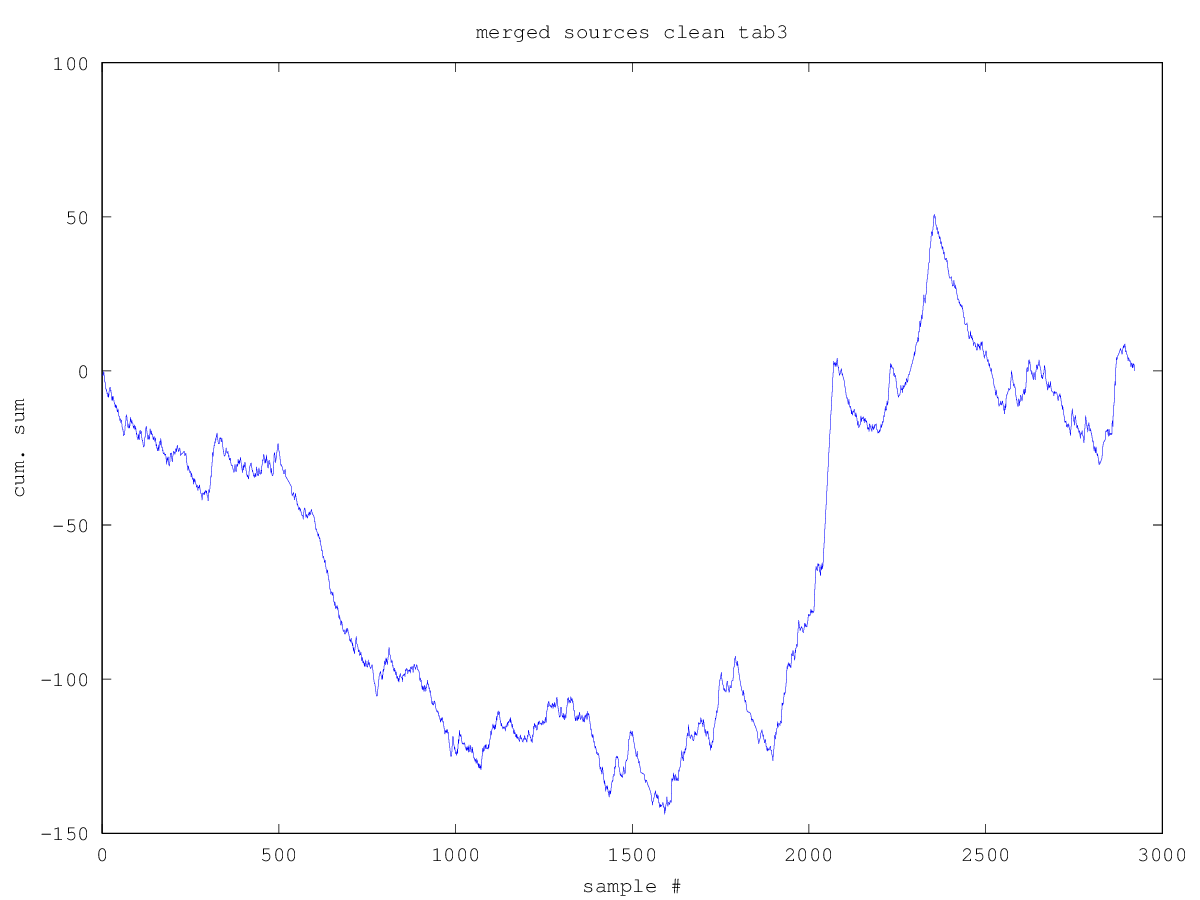
\includegraphics[width=0.8\linewidth]{{fractals/merged_data/merged_sources_clean_tab3_time_series}.png}
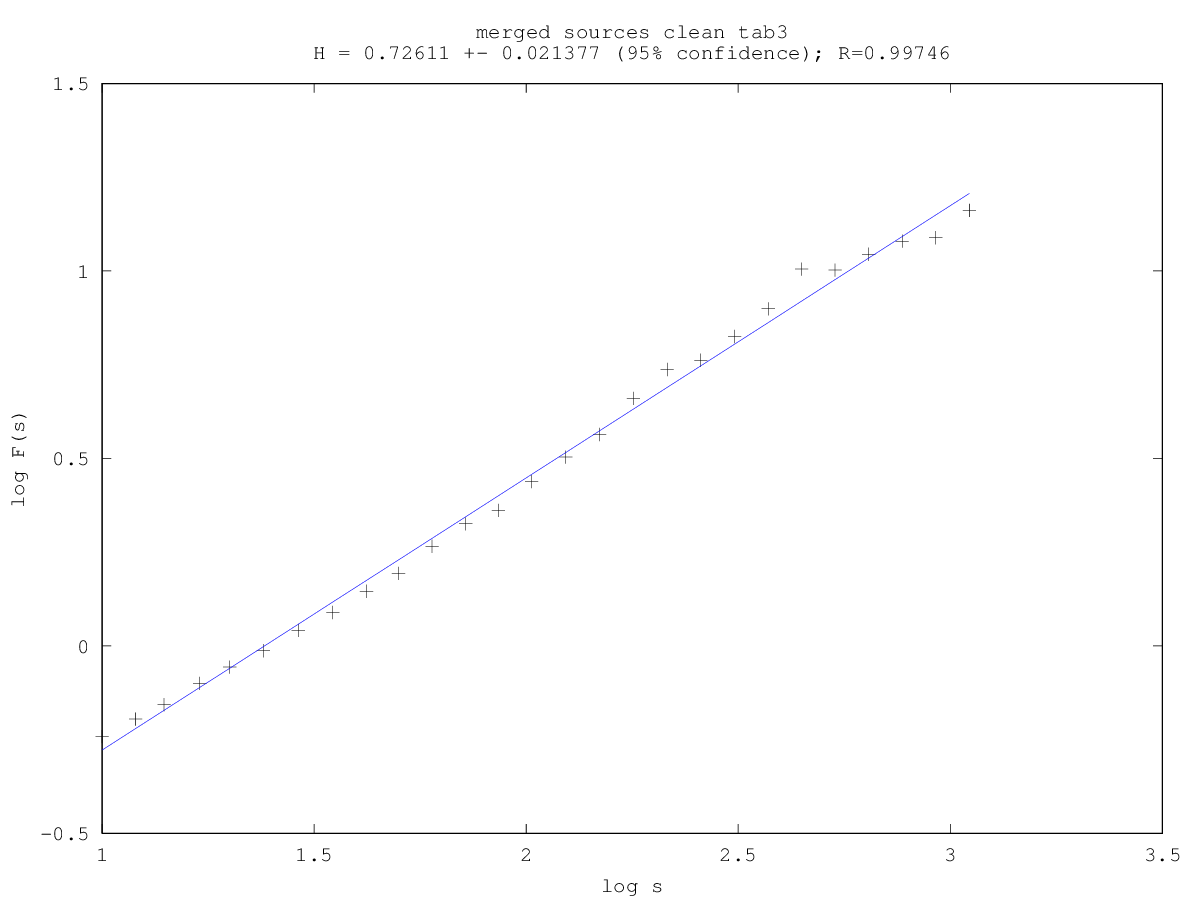
\includegraphics[width=0.8\linewidth]{{fractals/merged_data/merged_sources_clean_tab3_log_log}.png}
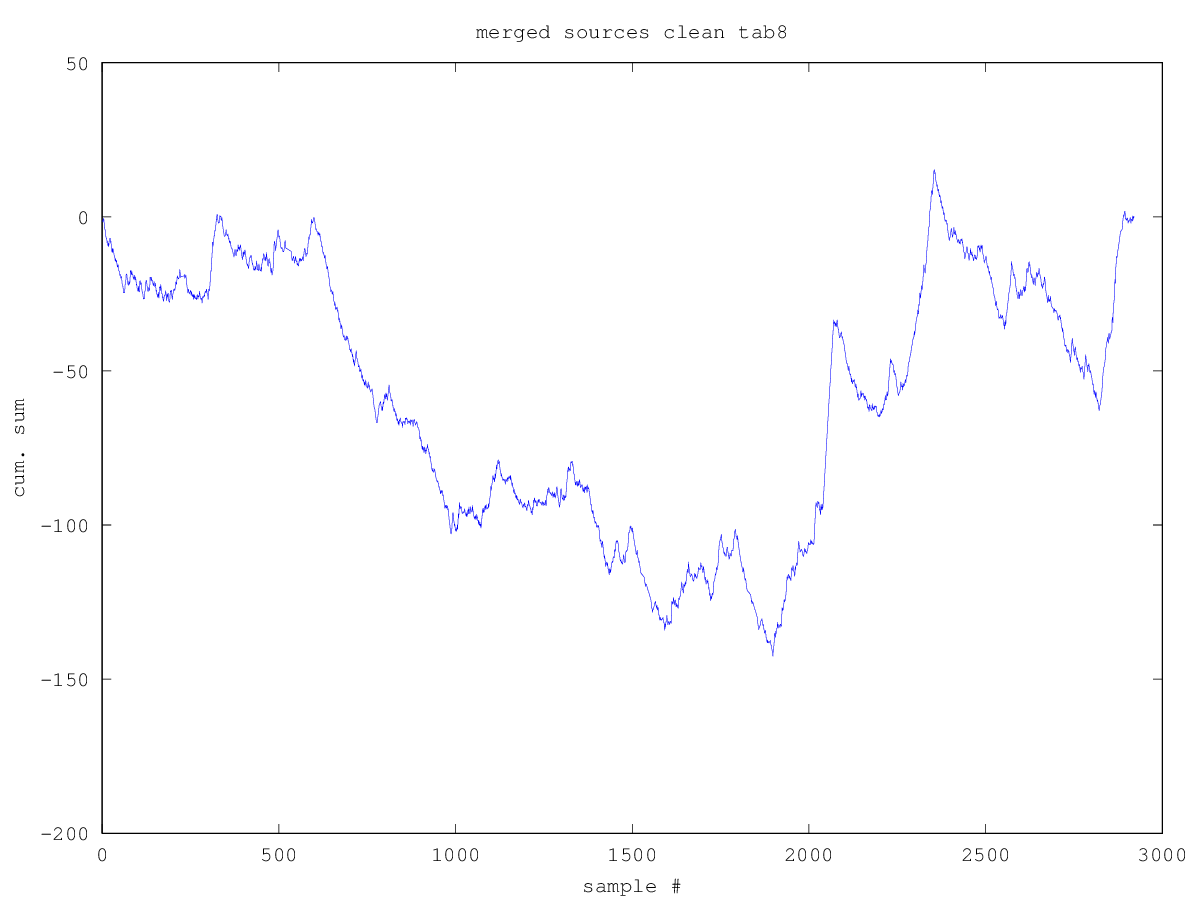
\includegraphics[width=0.8\linewidth]{{fractals/merged_data/merged_sources_clean_tab8_time_series}.png}
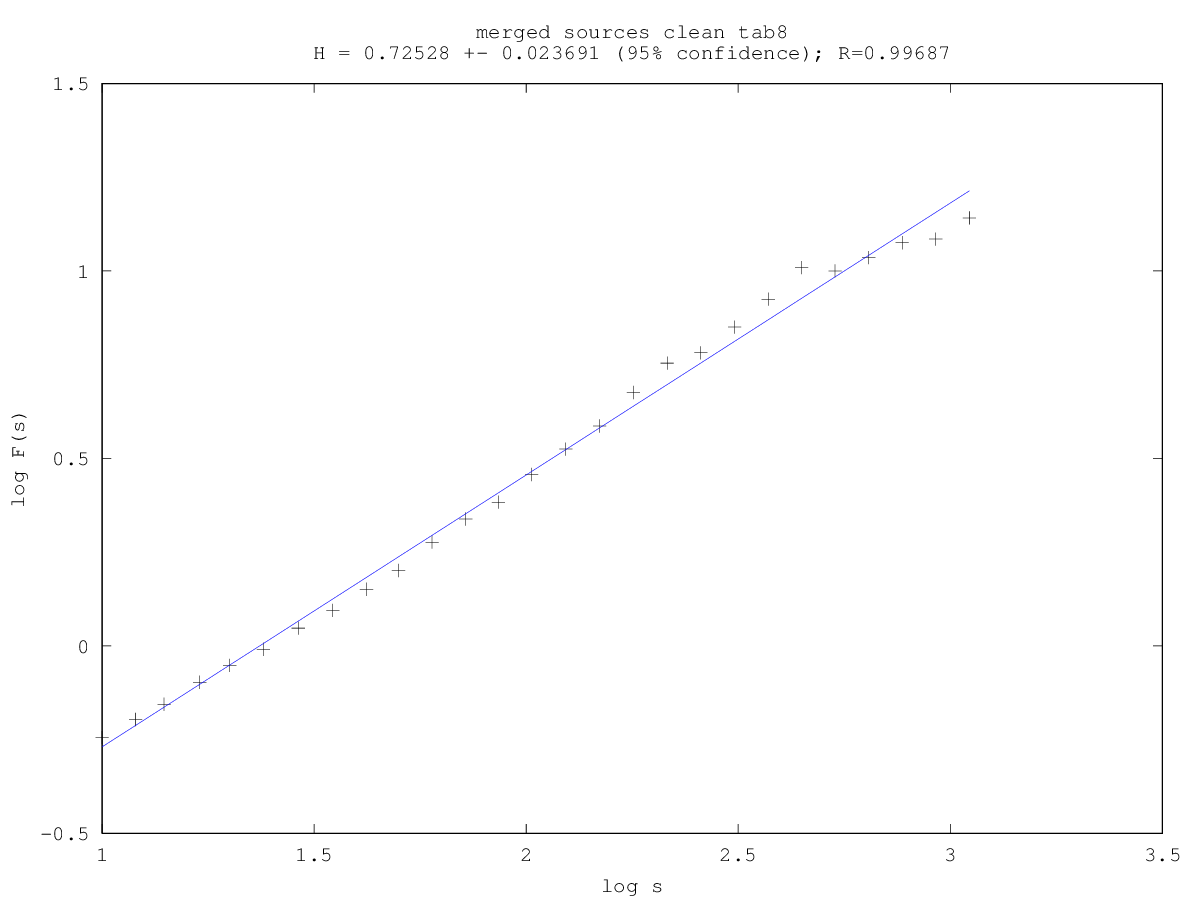
\includegraphics[width=0.8\linewidth]{{fractals/merged_data/merged_sources_clean_tab8_log_log}.png}
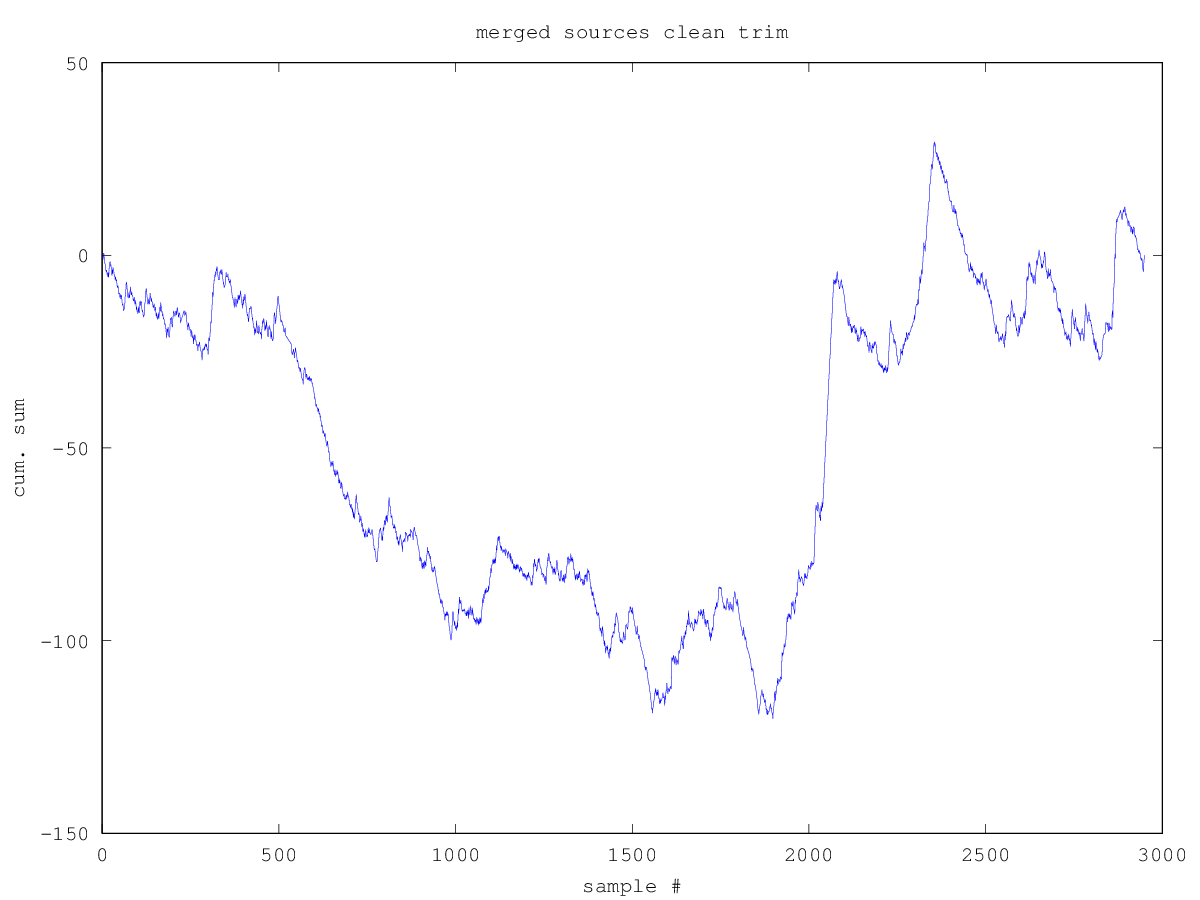
\includegraphics[width=0.8\linewidth]{{fractals/merged_data/merged_sources_clean_trim_time_series}.png}
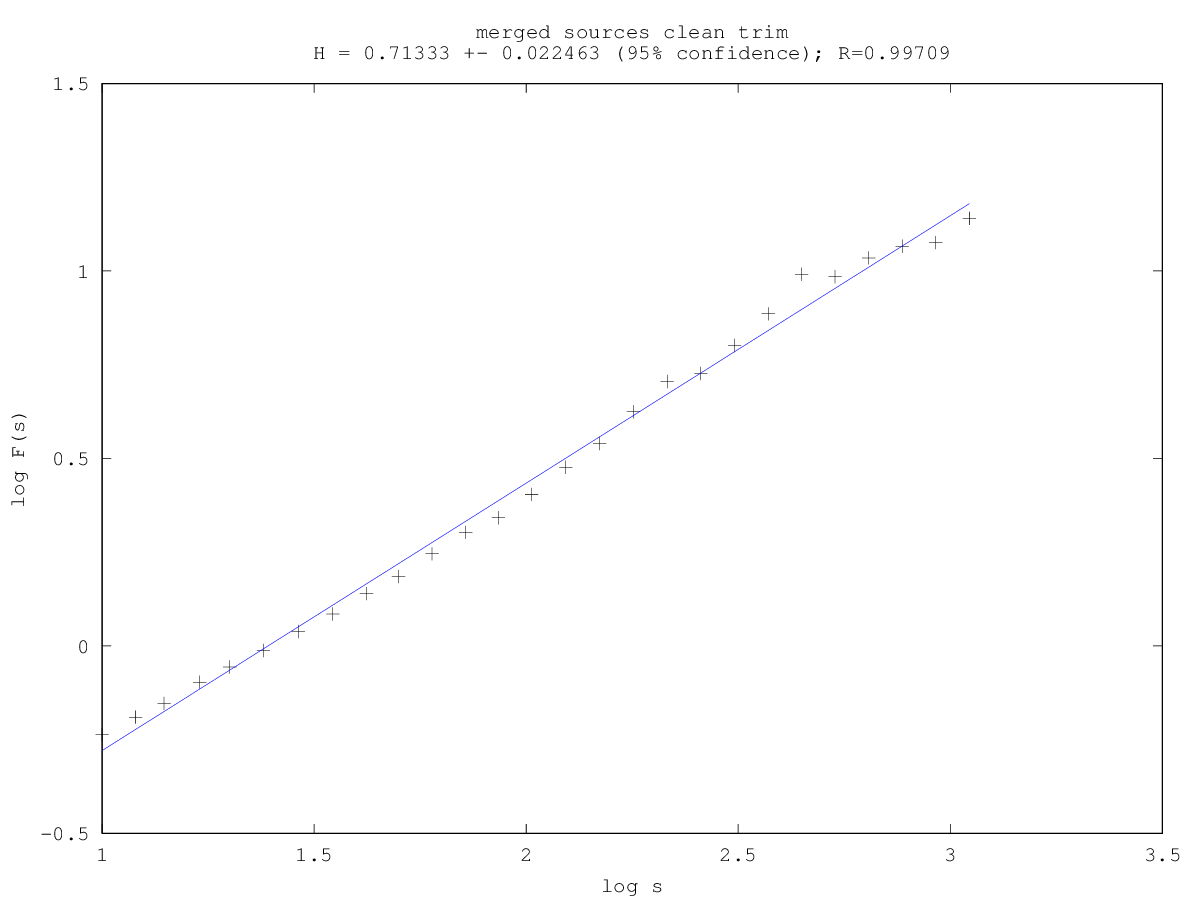
\includegraphics[width=0.8\linewidth]{{fractals/merged_data/merged_sources_clean_trim_log_log}.png}
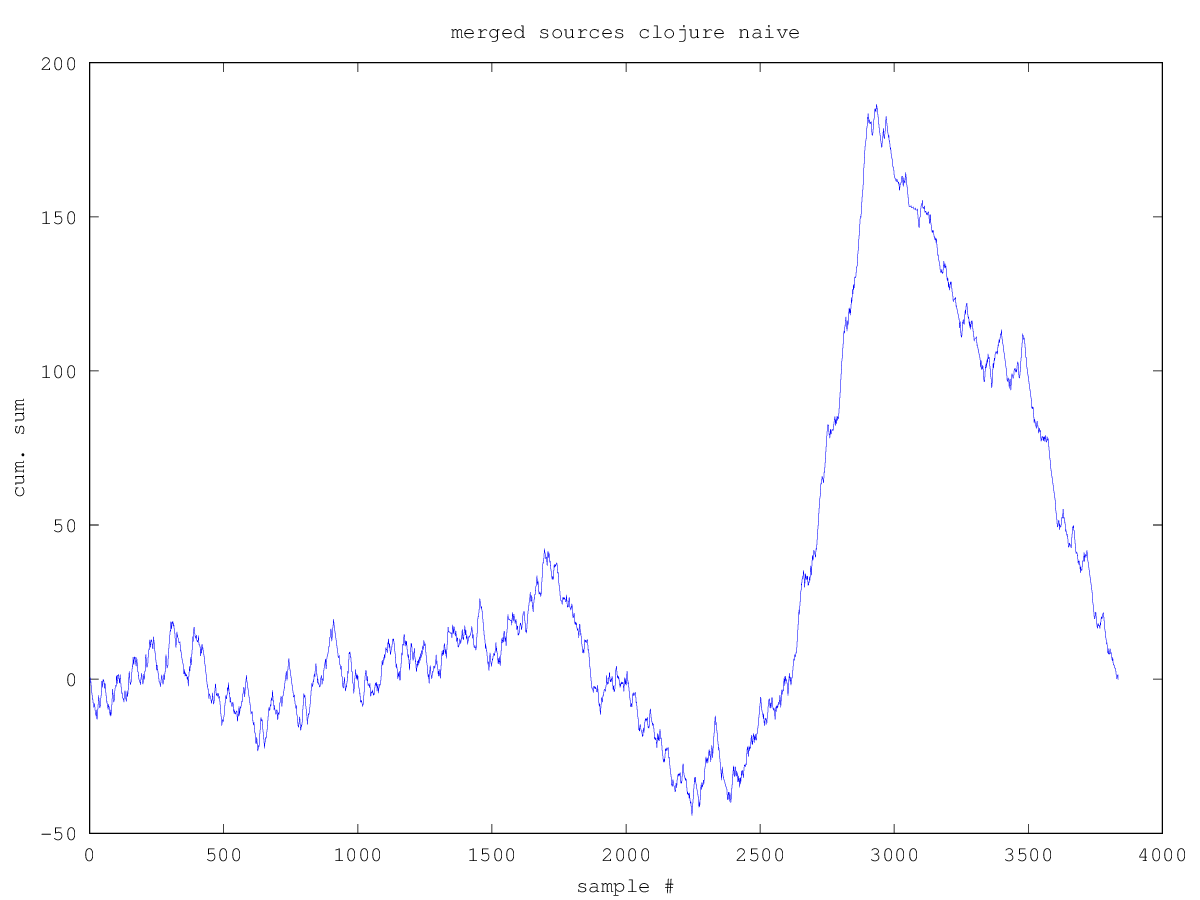
\includegraphics[width=0.8\linewidth]{{fractals/merged_data/merged_sources_clojure_naive_time_series}.png}
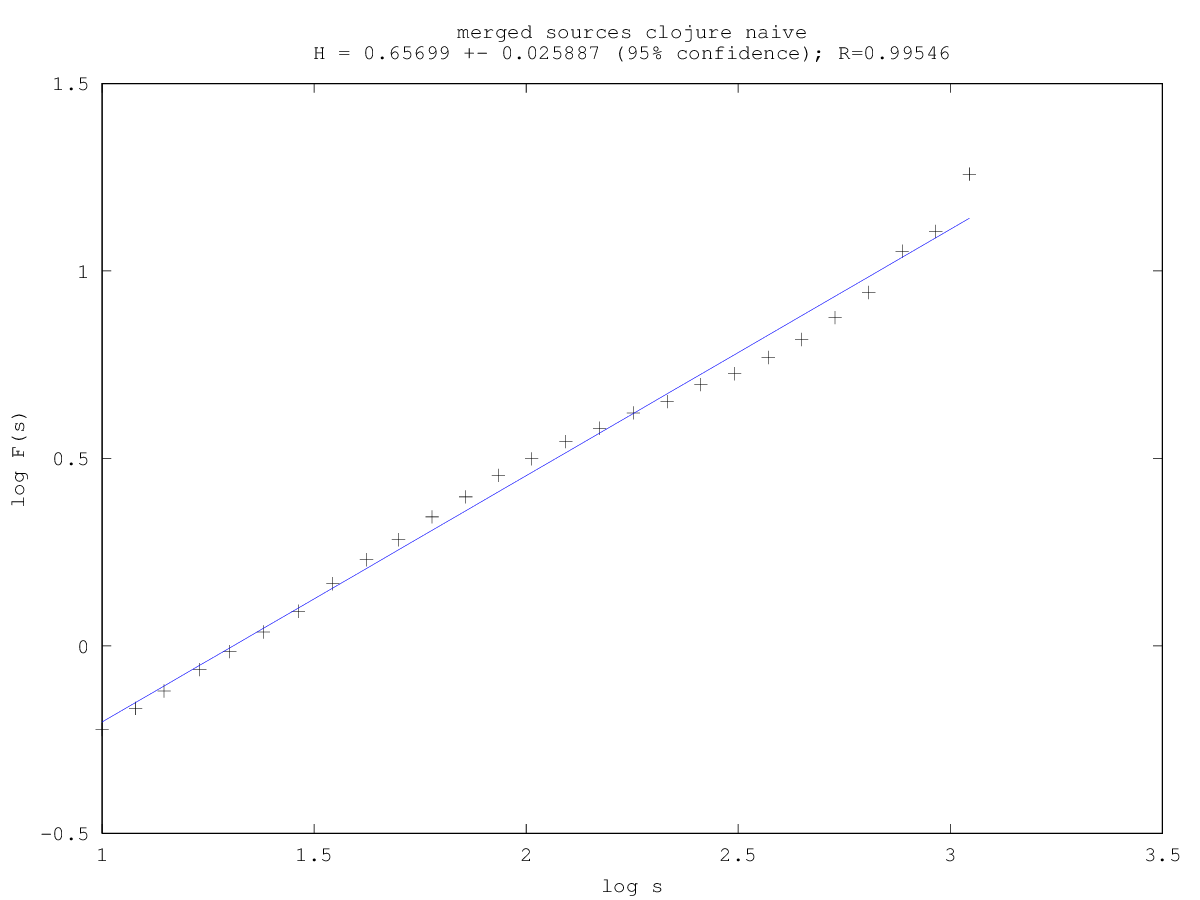
\includegraphics[width=0.8\linewidth]{{fractals/merged_data/merged_sources_clojure_naive_log_log}.png}
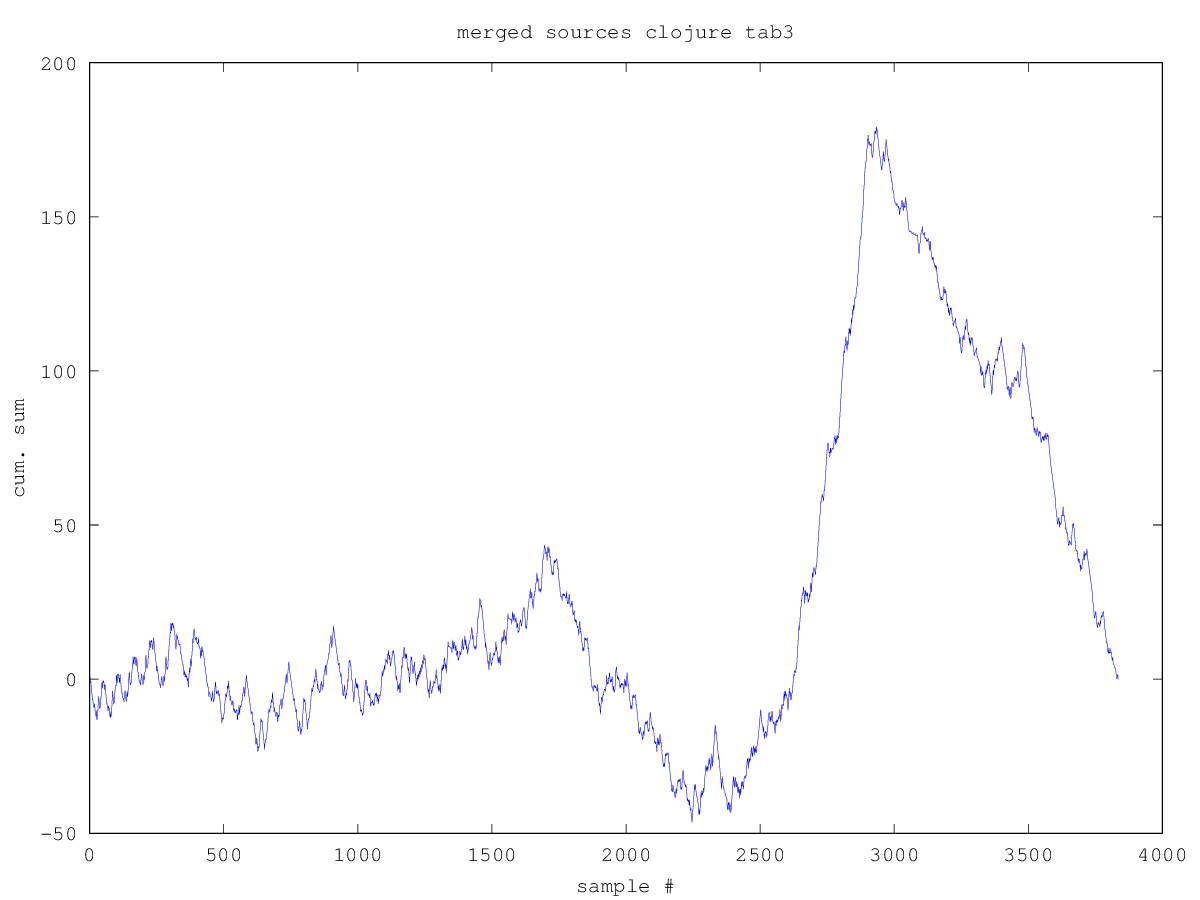
\includegraphics[width=0.8\linewidth]{{fractals/merged_data/merged_sources_clojure_tab3_time_series}.png}
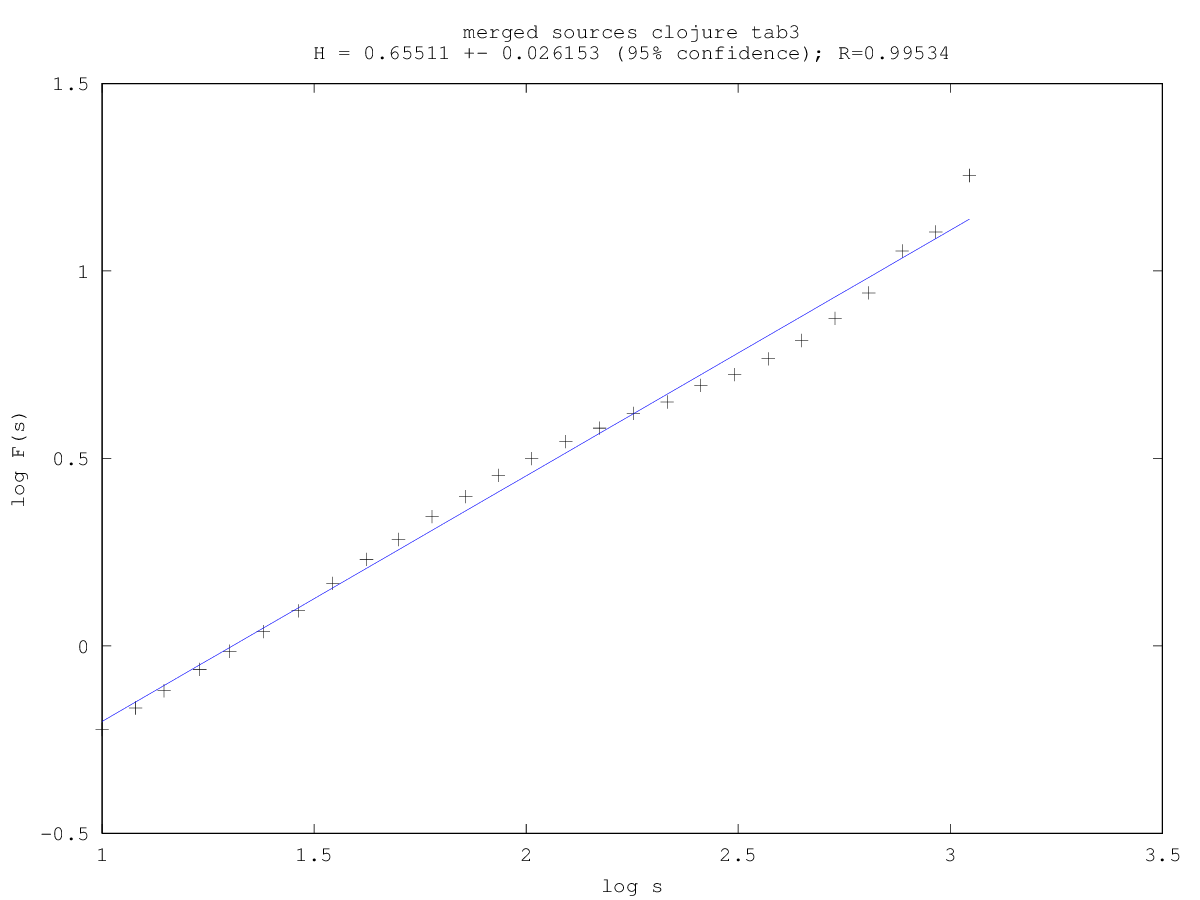
\includegraphics[width=0.8\linewidth]{{fractals/merged_data/merged_sources_clojure_tab3_log_log}.png}
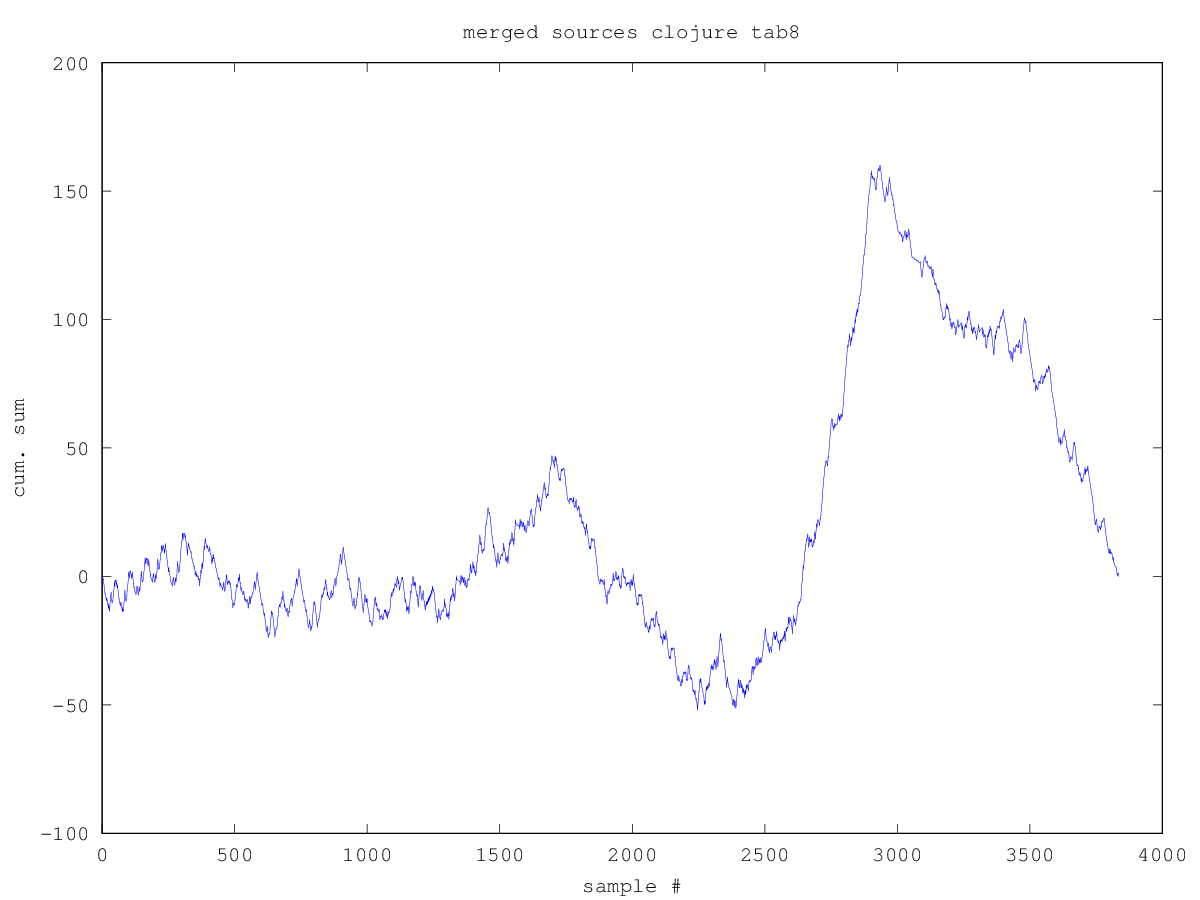
\includegraphics[width=0.8\linewidth]{{fractals/merged_data/merged_sources_clojure_tab8_time_series}.png}
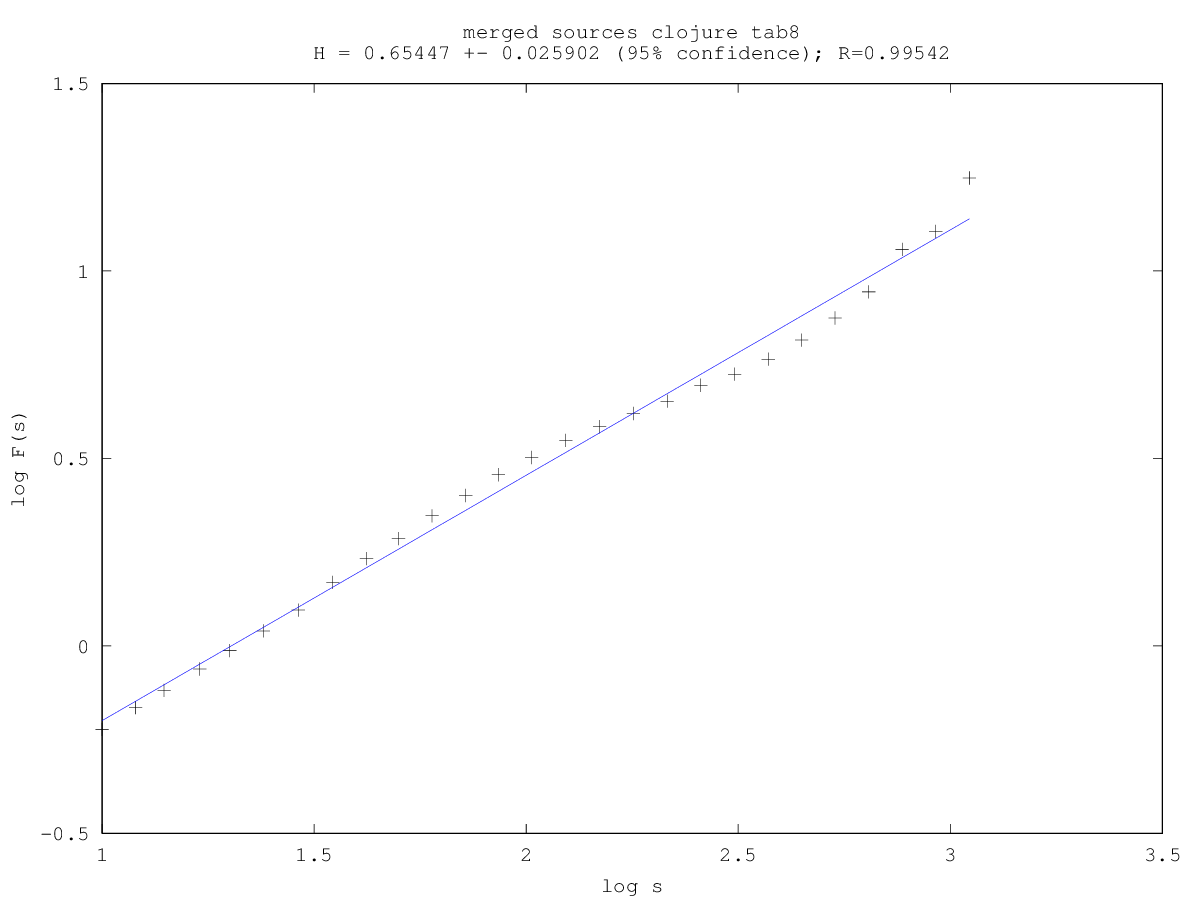
\includegraphics[width=0.8\linewidth]{{fractals/merged_data/merged_sources_clojure_tab8_log_log}.png}
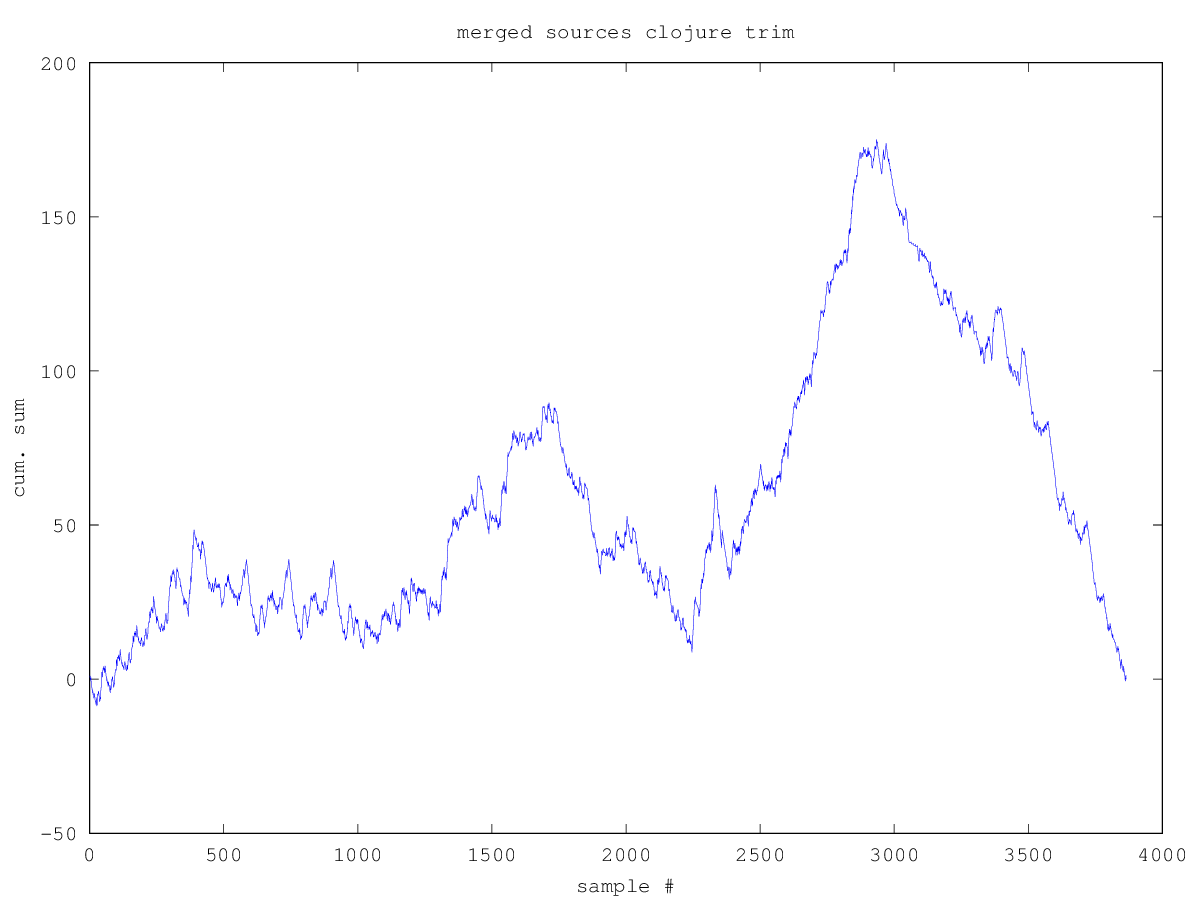
\includegraphics[width=0.8\linewidth]{{fractals/merged_data/merged_sources_clojure_trim_time_series}.png}
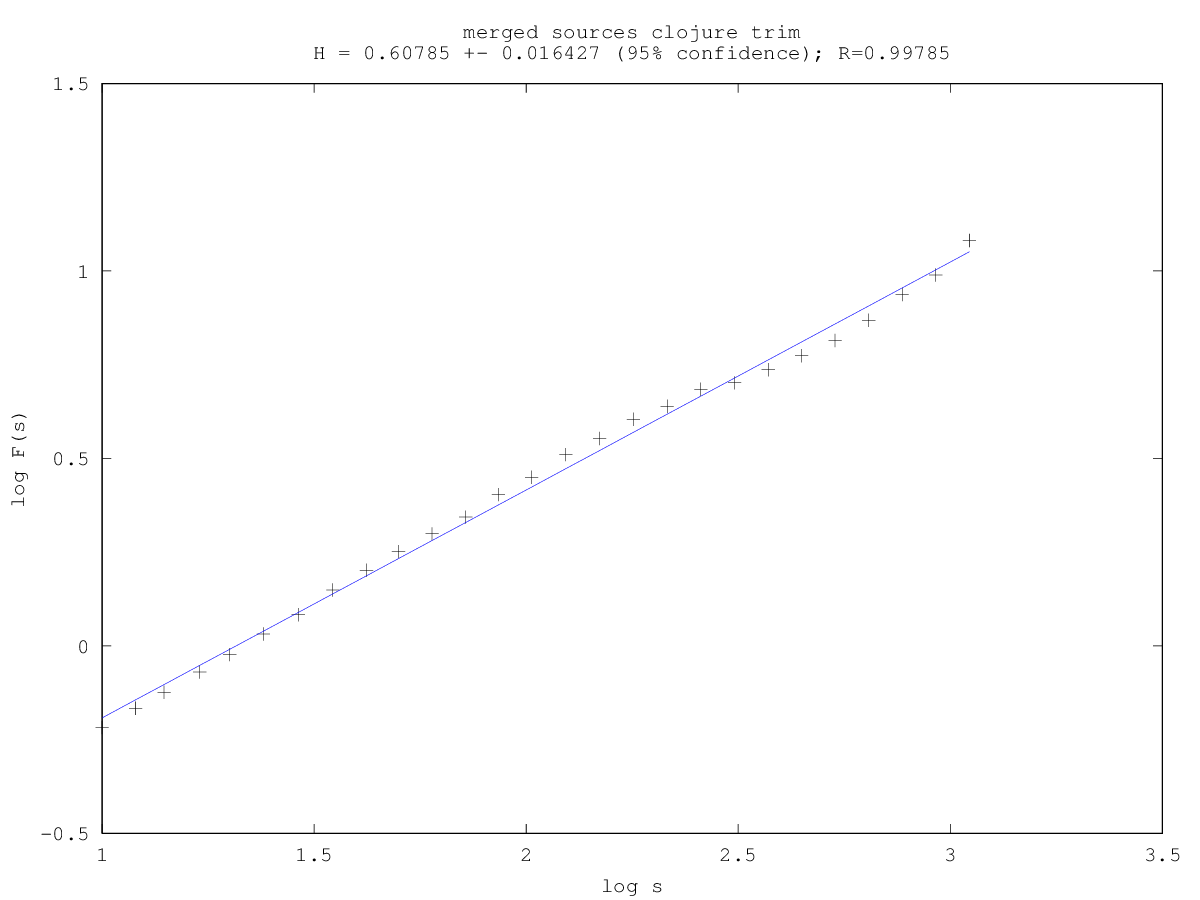
\includegraphics[width=0.8\linewidth]{{fractals/merged_data/merged_sources_clojure_trim_log_log}.png}
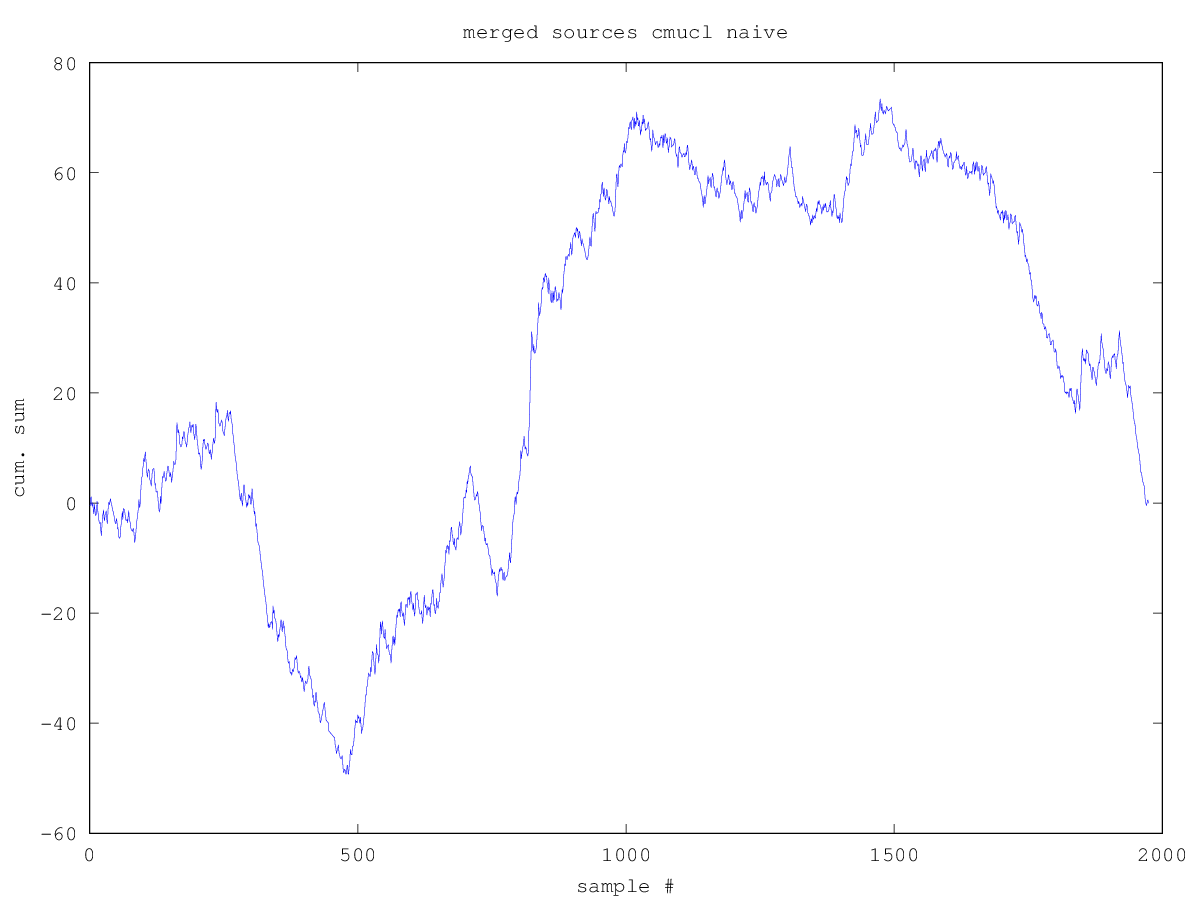
\includegraphics[width=0.8\linewidth]{{fractals/merged_data/merged_sources_cmucl_naive_time_series}.png}
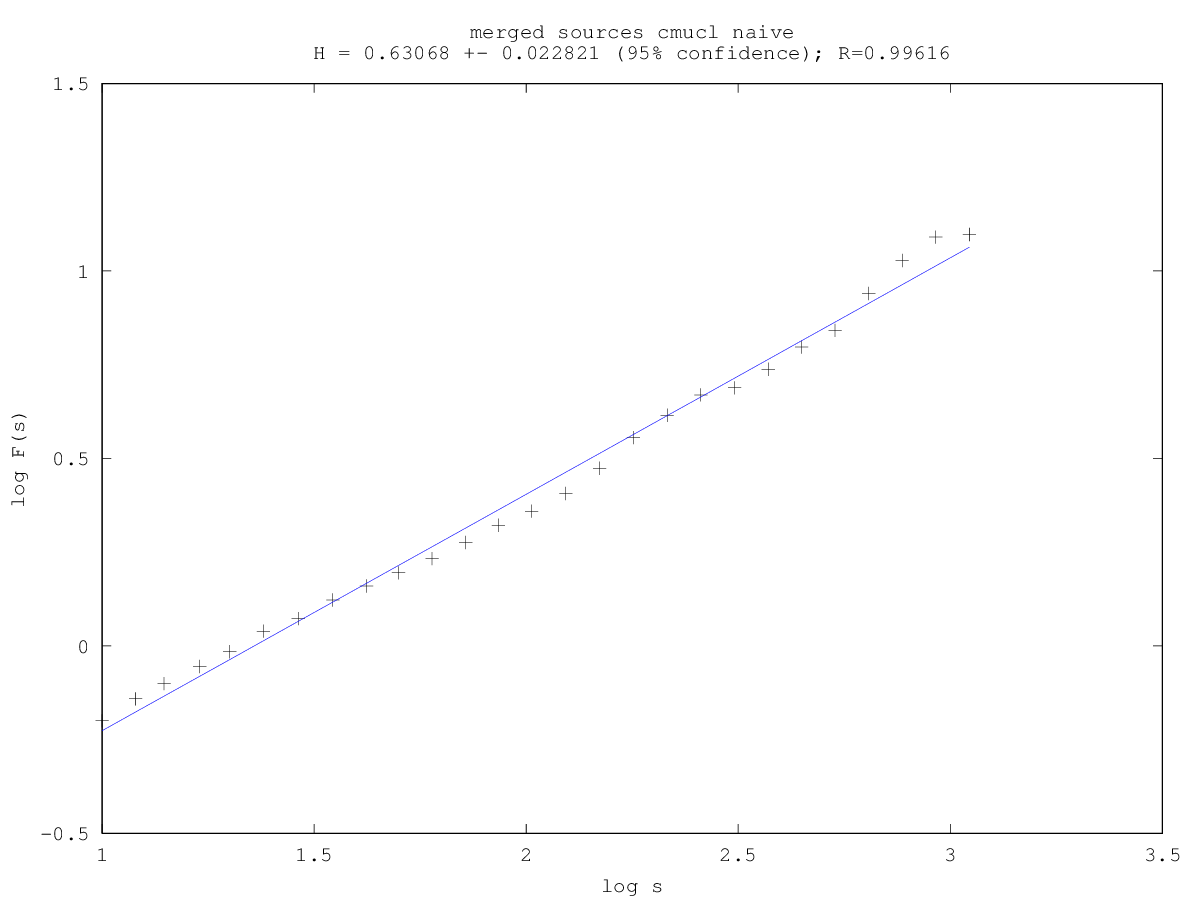
\includegraphics[width=0.8\linewidth]{{fractals/merged_data/merged_sources_cmucl_naive_log_log}.png}
\includegraphics[width=0.8\linewidth]{{fractals/merged_data/merged_sources_cmucl_tab3_time_series}.png}
\includegraphics[width=0.8\linewidth]{{fractals/merged_data/merged_sources_cmucl_tab3_log_log}.png}
\includegraphics[width=0.8\linewidth]{{fractals/merged_data/merged_sources_cmucl_tab8_time_series}.png}
\includegraphics[width=0.8\linewidth]{{fractals/merged_data/merged_sources_cmucl_tab8_log_log}.png}
\includegraphics[width=0.8\linewidth]{{fractals/merged_data/merged_sources_cmucl_trim_time_series}.png}
\includegraphics[width=0.8\linewidth]{{fractals/merged_data/merged_sources_cmucl_trim_log_log}.png}
\includegraphics[width=0.8\linewidth]{{fractals/merged_data/merged_sources_csharp_naive_time_series}.png}
\includegraphics[width=0.8\linewidth]{{fractals/merged_data/merged_sources_csharp_naive_log_log}.png}
\includegraphics[width=0.8\linewidth]{{fractals/merged_data/merged_sources_csharp_tab3_time_series}.png}
\includegraphics[width=0.8\linewidth]{{fractals/merged_data/merged_sources_csharp_tab3_log_log}.png}
\includegraphics[width=0.8\linewidth]{{fractals/merged_data/merged_sources_csharp_tab8_time_series}.png}
\includegraphics[width=0.8\linewidth]{{fractals/merged_data/merged_sources_csharp_tab8_log_log}.png}
\includegraphics[width=0.8\linewidth]{{fractals/merged_data/merged_sources_csharp_trim_time_series}.png}
\includegraphics[width=0.8\linewidth]{{fractals/merged_data/merged_sources_csharp_trim_log_log}.png}
\includegraphics[width=0.8\linewidth]{{fractals/merged_data/merged_sources_cyc_naive_time_series}.png}
\includegraphics[width=0.8\linewidth]{{fractals/merged_data/merged_sources_cyc_naive_log_log}.png}
\includegraphics[width=0.8\linewidth]{{fractals/merged_data/merged_sources_cyc_tab3_time_series}.png}
\includegraphics[width=0.8\linewidth]{{fractals/merged_data/merged_sources_cyc_tab3_log_log}.png}
\includegraphics[width=0.8\linewidth]{{fractals/merged_data/merged_sources_cyc_tab8_time_series}.png}
\includegraphics[width=0.8\linewidth]{{fractals/merged_data/merged_sources_cyc_tab8_log_log}.png}
\includegraphics[width=0.8\linewidth]{{fractals/merged_data/merged_sources_cyc_trim_time_series}.png}
\includegraphics[width=0.8\linewidth]{{fractals/merged_data/merged_sources_cyc_trim_log_log}.png}
\includegraphics[width=0.8\linewidth]{{fractals/merged_data/merged_sources_dlang_naive_time_series}.png}
\includegraphics[width=0.8\linewidth]{{fractals/merged_data/merged_sources_dlang_naive_log_log}.png}
\includegraphics[width=0.8\linewidth]{{fractals/merged_data/merged_sources_dlang_tab3_time_series}.png}
\includegraphics[width=0.8\linewidth]{{fractals/merged_data/merged_sources_dlang_tab3_log_log}.png}
\includegraphics[width=0.8\linewidth]{{fractals/merged_data/merged_sources_dlang_tab8_time_series}.png}
\includegraphics[width=0.8\linewidth]{{fractals/merged_data/merged_sources_dlang_tab8_log_log}.png}
\includegraphics[width=0.8\linewidth]{{fractals/merged_data/merged_sources_dlang_trim_time_series}.png}
\includegraphics[width=0.8\linewidth]{{fractals/merged_data/merged_sources_dlang_trim_log_log}.png}
\includegraphics[width=0.8\linewidth]{{fractals/merged_data/merged_sources_erlang_naive_time_series}.png}
\includegraphics[width=0.8\linewidth]{{fractals/merged_data/merged_sources_erlang_naive_log_log}.png}
\includegraphics[width=0.8\linewidth]{{fractals/merged_data/merged_sources_erlang_tab3_time_series}.png}
\includegraphics[width=0.8\linewidth]{{fractals/merged_data/merged_sources_erlang_tab3_log_log}.png}
\includegraphics[width=0.8\linewidth]{{fractals/merged_data/merged_sources_erlang_tab8_time_series}.png}
\includegraphics[width=0.8\linewidth]{{fractals/merged_data/merged_sources_erlang_tab8_log_log}.png}
\includegraphics[width=0.8\linewidth]{{fractals/merged_data/merged_sources_erlang_trim_time_series}.png}
\includegraphics[width=0.8\linewidth]{{fractals/merged_data/merged_sources_erlang_trim_log_log}.png}
\includegraphics[width=0.8\linewidth]{{fractals/merged_data/merged_sources_f90_naive_time_series}.png}
\includegraphics[width=0.8\linewidth]{{fractals/merged_data/merged_sources_f90_naive_log_log}.png}
\includegraphics[width=0.8\linewidth]{{fractals/merged_data/merged_sources_f90_tab3_time_series}.png}
\includegraphics[width=0.8\linewidth]{{fractals/merged_data/merged_sources_f90_tab3_log_log}.png}
\includegraphics[width=0.8\linewidth]{{fractals/merged_data/merged_sources_f90_tab8_time_series}.png}
\includegraphics[width=0.8\linewidth]{{fractals/merged_data/merged_sources_f90_tab8_log_log}.png}
\includegraphics[width=0.8\linewidth]{{fractals/merged_data/merged_sources_f90_trim_time_series}.png}
\includegraphics[width=0.8\linewidth]{{fractals/merged_data/merged_sources_f90_trim_log_log}.png}
\includegraphics[width=0.8\linewidth]{{fractals/merged_data/merged_sources_fbasic_naive_time_series}.png}
\includegraphics[width=0.8\linewidth]{{fractals/merged_data/merged_sources_fbasic_naive_log_log}.png}
\includegraphics[width=0.8\linewidth]{{fractals/merged_data/merged_sources_fbasic_tab3_time_series}.png}
\includegraphics[width=0.8\linewidth]{{fractals/merged_data/merged_sources_fbasic_tab3_log_log}.png}
\includegraphics[width=0.8\linewidth]{{fractals/merged_data/merged_sources_fbasic_tab8_time_series}.png}
\includegraphics[width=0.8\linewidth]{{fractals/merged_data/merged_sources_fbasic_tab8_log_log}.png}
\includegraphics[width=0.8\linewidth]{{fractals/merged_data/merged_sources_fbasic_trim_time_series}.png}
\includegraphics[width=0.8\linewidth]{{fractals/merged_data/merged_sources_fbasic_trim_log_log}.png}
\includegraphics[width=0.8\linewidth]{{fractals/merged_data/merged_sources_fpascal_naive_time_series}.png}
\includegraphics[width=0.8\linewidth]{{fractals/merged_data/merged_sources_fpascal_naive_log_log}.png}
\includegraphics[width=0.8\linewidth]{{fractals/merged_data/merged_sources_fpascal_tab3_time_series}.png}
\includegraphics[width=0.8\linewidth]{{fractals/merged_data/merged_sources_fpascal_tab3_log_log}.png}
\includegraphics[width=0.8\linewidth]{{fractals/merged_data/merged_sources_fpascal_tab8_time_series}.png}
\includegraphics[width=0.8\linewidth]{{fractals/merged_data/merged_sources_fpascal_tab8_log_log}.png}
\includegraphics[width=0.8\linewidth]{{fractals/merged_data/merged_sources_fpascal_trim_time_series}.png}
\includegraphics[width=0.8\linewidth]{{fractals/merged_data/merged_sources_fpascal_trim_log_log}.png}
\includegraphics[width=0.8\linewidth]{{fractals/merged_data/merged_sources_gcc_naive_time_series}.png}
\includegraphics[width=0.8\linewidth]{{fractals/merged_data/merged_sources_gcc_naive_log_log}.png}
\includegraphics[width=0.8\linewidth]{{fractals/merged_data/merged_sources_gcc_tab3_time_series}.png}
\includegraphics[width=0.8\linewidth]{{fractals/merged_data/merged_sources_gcc_tab3_log_log}.png}
\includegraphics[width=0.8\linewidth]{{fractals/merged_data/merged_sources_gcc_tab8_time_series}.png}
\includegraphics[width=0.8\linewidth]{{fractals/merged_data/merged_sources_gcc_tab8_log_log}.png}
\includegraphics[width=0.8\linewidth]{{fractals/merged_data/merged_sources_gcc_trim_time_series}.png}
\includegraphics[width=0.8\linewidth]{{fractals/merged_data/merged_sources_gcc_trim_log_log}.png}
\includegraphics[width=0.8\linewidth]{{fractals/merged_data/merged_sources_gforth_naive_time_series}.png}
\includegraphics[width=0.8\linewidth]{{fractals/merged_data/merged_sources_gforth_naive_log_log}.png}
\includegraphics[width=0.8\linewidth]{{fractals/merged_data/merged_sources_ghc_naive_time_series}.png}
\includegraphics[width=0.8\linewidth]{{fractals/merged_data/merged_sources_ghc_naive_log_log}.png}
\includegraphics[width=0.8\linewidth]{{fractals/merged_data/merged_sources_ghc_tab3_time_series}.png}
\includegraphics[width=0.8\linewidth]{{fractals/merged_data/merged_sources_ghc_tab3_log_log}.png}
\includegraphics[width=0.8\linewidth]{{fractals/merged_data/merged_sources_ghc_tab8_time_series}.png}
\includegraphics[width=0.8\linewidth]{{fractals/merged_data/merged_sources_ghc_tab8_log_log}.png}
\includegraphics[width=0.8\linewidth]{{fractals/merged_data/merged_sources_ghc_trim_time_series}.png}
\includegraphics[width=0.8\linewidth]{{fractals/merged_data/merged_sources_ghc_trim_log_log}.png}
\includegraphics[width=0.8\linewidth]{{fractals/merged_data/merged_sources_gnat_naive_time_series}.png}
\includegraphics[width=0.8\linewidth]{{fractals/merged_data/merged_sources_gnat_naive_log_log}.png}
\includegraphics[width=0.8\linewidth]{{fractals/merged_data/merged_sources_gnat_tab3_time_series}.png}
\includegraphics[width=0.8\linewidth]{{fractals/merged_data/merged_sources_gnat_tab3_log_log}.png}
\includegraphics[width=0.8\linewidth]{{fractals/merged_data/merged_sources_gnat_tab8_time_series}.png}
\includegraphics[width=0.8\linewidth]{{fractals/merged_data/merged_sources_gnat_tab8_log_log}.png}
\includegraphics[width=0.8\linewidth]{{fractals/merged_data/merged_sources_gnat_trim_time_series}.png}
\includegraphics[width=0.8\linewidth]{{fractals/merged_data/merged_sources_gnat_trim_log_log}.png}
\includegraphics[width=0.8\linewidth]{{fractals/merged_data/merged_sources_go_naive_time_series}.png}
\includegraphics[width=0.8\linewidth]{{fractals/merged_data/merged_sources_go_naive_log_log}.png}
\includegraphics[width=0.8\linewidth]{{fractals/merged_data/merged_sources_go_tab3_time_series}.png}
\includegraphics[width=0.8\linewidth]{{fractals/merged_data/merged_sources_go_tab3_log_log}.png}
\includegraphics[width=0.8\linewidth]{{fractals/merged_data/merged_sources_go_tab8_time_series}.png}
\includegraphics[width=0.8\linewidth]{{fractals/merged_data/merged_sources_go_tab8_log_log}.png}
\includegraphics[width=0.8\linewidth]{{fractals/merged_data/merged_sources_go_trim_time_series}.png}
\includegraphics[width=0.8\linewidth]{{fractals/merged_data/merged_sources_go_trim_log_log}.png}
\includegraphics[width=0.8\linewidth]{{fractals/merged_data/merged_sources_gpp_naive_time_series}.png}
\includegraphics[width=0.8\linewidth]{{fractals/merged_data/merged_sources_gpp_naive_log_log}.png}
\includegraphics[width=0.8\linewidth]{{fractals/merged_data/merged_sources_gst_naive_time_series}.png}
\includegraphics[width=0.8\linewidth]{{fractals/merged_data/merged_sources_gst_naive_log_log}.png}
\includegraphics[width=0.8\linewidth]{{fractals/merged_data/merged_sources_gst_tab3_time_series}.png}
\includegraphics[width=0.8\linewidth]{{fractals/merged_data/merged_sources_gst_tab3_log_log}.png}
\includegraphics[width=0.8\linewidth]{{fractals/merged_data/merged_sources_gst_tab8_time_series}.png}
\includegraphics[width=0.8\linewidth]{{fractals/merged_data/merged_sources_gst_tab8_log_log}.png}
\includegraphics[width=0.8\linewidth]{{fractals/merged_data/merged_sources_gst_trim_time_series}.png}
\includegraphics[width=0.8\linewidth]{{fractals/merged_data/merged_sources_gst_trim_log_log}.png}
\includegraphics[width=0.8\linewidth]{{fractals/merged_data/merged_sources_ifc_naive_time_series}.png}
\includegraphics[width=0.8\linewidth]{{fractals/merged_data/merged_sources_ifc_naive_log_log}.png}
\includegraphics[width=0.8\linewidth]{{fractals/merged_data/merged_sources_ifc_tab3_time_series}.png}
\includegraphics[width=0.8\linewidth]{{fractals/merged_data/merged_sources_ifc_tab3_log_log}.png}
\includegraphics[width=0.8\linewidth]{{fractals/merged_data/merged_sources_ifc_tab8_time_series}.png}
\includegraphics[width=0.8\linewidth]{{fractals/merged_data/merged_sources_ifc_tab8_log_log}.png}
\includegraphics[width=0.8\linewidth]{{fractals/merged_data/merged_sources_ifc_trim_time_series}.png}
\includegraphics[width=0.8\linewidth]{{fractals/merged_data/merged_sources_ifc_trim_log_log}.png}
\includegraphics[width=0.8\linewidth]{{fractals/merged_data/merged_sources_java14_naive_time_series}.png}
\includegraphics[width=0.8\linewidth]{{fractals/merged_data/merged_sources_java14_naive_log_log}.png}
\includegraphics[width=0.8\linewidth]{{fractals/merged_data/merged_sources_java14_tab3_time_series}.png}
\includegraphics[width=0.8\linewidth]{{fractals/merged_data/merged_sources_java14_tab3_log_log}.png}
\includegraphics[width=0.8\linewidth]{{fractals/merged_data/merged_sources_java14_tab8_time_series}.png}
\includegraphics[width=0.8\linewidth]{{fractals/merged_data/merged_sources_java14_tab8_log_log}.png}
\includegraphics[width=0.8\linewidth]{{fractals/merged_data/merged_sources_java14_trim_time_series}.png}
\includegraphics[width=0.8\linewidth]{{fractals/merged_data/merged_sources_java14_trim_log_log}.png}
\includegraphics[width=0.8\linewidth]{{fractals/merged_data/merged_sources_java_naive_time_series}.png}
\includegraphics[width=0.8\linewidth]{{fractals/merged_data/merged_sources_java_naive_log_log}.png}
\includegraphics[width=0.8\linewidth]{{fractals/merged_data/merged_sources_java_tab3_time_series}.png}
\includegraphics[width=0.8\linewidth]{{fractals/merged_data/merged_sources_java_tab3_log_log}.png}
\includegraphics[width=0.8\linewidth]{{fractals/merged_data/merged_sources_java_tab8_time_series}.png}
\includegraphics[width=0.8\linewidth]{{fractals/merged_data/merged_sources_java_tab8_log_log}.png}
\includegraphics[width=0.8\linewidth]{{fractals/merged_data/merged_sources_java_trim_time_series}.png}
\includegraphics[width=0.8\linewidth]{{fractals/merged_data/merged_sources_java_trim_log_log}.png}
\includegraphics[width=0.8\linewidth]{{fractals/merged_data/merged_sources_javasteady_naive_time_series}.png}
\includegraphics[width=0.8\linewidth]{{fractals/merged_data/merged_sources_javasteady_naive_log_log}.png}
\includegraphics[width=0.8\linewidth]{{fractals/merged_data/merged_sources_javasteady_tab3_time_series}.png}
\includegraphics[width=0.8\linewidth]{{fractals/merged_data/merged_sources_javasteady_tab3_log_log}.png}
\includegraphics[width=0.8\linewidth]{{fractals/merged_data/merged_sources_javasteady_tab8_time_series}.png}
\includegraphics[width=0.8\linewidth]{{fractals/merged_data/merged_sources_javasteady_tab8_log_log}.png}
\includegraphics[width=0.8\linewidth]{{fractals/merged_data/merged_sources_javasteady_trim_time_series}.png}
\includegraphics[width=0.8\linewidth]{{fractals/merged_data/merged_sources_javasteady_trim_log_log}.png}
\includegraphics[width=0.8\linewidth]{{fractals/merged_data/merged_sources_jruby_naive_time_series}.png}
\includegraphics[width=0.8\linewidth]{{fractals/merged_data/merged_sources_jruby_naive_log_log}.png}
\includegraphics[width=0.8\linewidth]{{fractals/merged_data/merged_sources_jruby_tab3_time_series}.png}
\includegraphics[width=0.8\linewidth]{{fractals/merged_data/merged_sources_jruby_tab3_log_log}.png}
\includegraphics[width=0.8\linewidth]{{fractals/merged_data/merged_sources_jruby_tab8_time_series}.png}
\includegraphics[width=0.8\linewidth]{{fractals/merged_data/merged_sources_jruby_tab8_log_log}.png}
\includegraphics[width=0.8\linewidth]{{fractals/merged_data/merged_sources_jruby_trim_time_series}.png}
\includegraphics[width=0.8\linewidth]{{fractals/merged_data/merged_sources_jruby_trim_log_log}.png}
\includegraphics[width=0.8\linewidth]{{fractals/merged_data/merged_sources_lisaac_naive_time_series}.png}
\includegraphics[width=0.8\linewidth]{{fractals/merged_data/merged_sources_lisaac_naive_log_log}.png}
\includegraphics[width=0.8\linewidth]{{fractals/merged_data/merged_sources_lisaac_tab3_time_series}.png}
\includegraphics[width=0.8\linewidth]{{fractals/merged_data/merged_sources_lisaac_tab3_log_log}.png}
\includegraphics[width=0.8\linewidth]{{fractals/merged_data/merged_sources_lisaac_tab8_time_series}.png}
\includegraphics[width=0.8\linewidth]{{fractals/merged_data/merged_sources_lisaac_tab8_log_log}.png}
\includegraphics[width=0.8\linewidth]{{fractals/merged_data/merged_sources_lisaac_trim_time_series}.png}
\includegraphics[width=0.8\linewidth]{{fractals/merged_data/merged_sources_lisaac_trim_log_log}.png}
\includegraphics[width=0.8\linewidth]{{fractals/merged_data/merged_sources_lua_naive_time_series}.png}
\includegraphics[width=0.8\linewidth]{{fractals/merged_data/merged_sources_lua_naive_log_log}.png}
\includegraphics[width=0.8\linewidth]{{fractals/merged_data/merged_sources_lua_tab3_time_series}.png}
\includegraphics[width=0.8\linewidth]{{fractals/merged_data/merged_sources_lua_tab3_log_log}.png}
\includegraphics[width=0.8\linewidth]{{fractals/merged_data/merged_sources_lua_tab8_time_series}.png}
\includegraphics[width=0.8\linewidth]{{fractals/merged_data/merged_sources_lua_tab8_log_log}.png}
\includegraphics[width=0.8\linewidth]{{fractals/merged_data/merged_sources_lua_trim_time_series}.png}
\includegraphics[width=0.8\linewidth]{{fractals/merged_data/merged_sources_lua_trim_log_log}.png}
\includegraphics[width=0.8\linewidth]{{fractals/merged_data/merged_sources_mercury_naive_time_series}.png}
\includegraphics[width=0.8\linewidth]{{fractals/merged_data/merged_sources_mercury_naive_log_log}.png}
\includegraphics[width=0.8\linewidth]{{fractals/merged_data/merged_sources_mercury_tab3_time_series}.png}
\includegraphics[width=0.8\linewidth]{{fractals/merged_data/merged_sources_mercury_tab3_log_log}.png}
\includegraphics[width=0.8\linewidth]{{fractals/merged_data/merged_sources_mercury_tab8_time_series}.png}
\includegraphics[width=0.8\linewidth]{{fractals/merged_data/merged_sources_mercury_tab8_log_log}.png}
\includegraphics[width=0.8\linewidth]{{fractals/merged_data/merged_sources_mercury_trim_time_series}.png}
\includegraphics[width=0.8\linewidth]{{fractals/merged_data/merged_sources_mercury_trim_log_log}.png}
\includegraphics[width=0.8\linewidth]{{fractals/merged_data/merged_sources_mlton_naive_time_series}.png}
\includegraphics[width=0.8\linewidth]{{fractals/merged_data/merged_sources_mlton_naive_log_log}.png}
\includegraphics[width=0.8\linewidth]{{fractals/merged_data/merged_sources_mlton_tab3_time_series}.png}
\includegraphics[width=0.8\linewidth]{{fractals/merged_data/merged_sources_mlton_tab3_log_log}.png}
\includegraphics[width=0.8\linewidth]{{fractals/merged_data/merged_sources_mlton_tab8_time_series}.png}
\includegraphics[width=0.8\linewidth]{{fractals/merged_data/merged_sources_mlton_tab8_log_log}.png}
\includegraphics[width=0.8\linewidth]{{fractals/merged_data/merged_sources_mlton_trim_time_series}.png}
\includegraphics[width=0.8\linewidth]{{fractals/merged_data/merged_sources_mlton_trim_log_log}.png}
\includegraphics[width=0.8\linewidth]{{fractals/merged_data/merged_sources_mzscheme_naive_time_series}.png}
\includegraphics[width=0.8\linewidth]{{fractals/merged_data/merged_sources_mzscheme_naive_log_log}.png}
\includegraphics[width=0.8\linewidth]{{fractals/merged_data/merged_sources_mzscheme_tab3_time_series}.png}
\includegraphics[width=0.8\linewidth]{{fractals/merged_data/merged_sources_mzscheme_tab3_log_log}.png}
\includegraphics[width=0.8\linewidth]{{fractals/merged_data/merged_sources_mzscheme_tab8_time_series}.png}
\includegraphics[width=0.8\linewidth]{{fractals/merged_data/merged_sources_mzscheme_tab8_log_log}.png}
\includegraphics[width=0.8\linewidth]{{fractals/merged_data/merged_sources_mzscheme_trim_time_series}.png}
\includegraphics[width=0.8\linewidth]{{fractals/merged_data/merged_sources_mzscheme_trim_log_log}.png}
\includegraphics[width=0.8\linewidth]{{fractals/merged_data/merged_sources_nice_naive_time_series}.png}
\includegraphics[width=0.8\linewidth]{{fractals/merged_data/merged_sources_nice_naive_log_log}.png}
\includegraphics[width=0.8\linewidth]{{fractals/merged_data/merged_sources_nice_tab3_time_series}.png}
\includegraphics[width=0.8\linewidth]{{fractals/merged_data/merged_sources_nice_tab3_log_log}.png}
\includegraphics[width=0.8\linewidth]{{fractals/merged_data/merged_sources_nice_tab8_time_series}.png}
\includegraphics[width=0.8\linewidth]{{fractals/merged_data/merged_sources_nice_tab8_log_log}.png}
\includegraphics[width=0.8\linewidth]{{fractals/merged_data/merged_sources_nice_trim_time_series}.png}
\includegraphics[width=0.8\linewidth]{{fractals/merged_data/merged_sources_nice_trim_log_log}.png}
\includegraphics[width=0.8\linewidth]{{fractals/merged_data/merged_sources_ocaml_naive_time_series}.png}
\includegraphics[width=0.8\linewidth]{{fractals/merged_data/merged_sources_ocaml_naive_log_log}.png}
\includegraphics[width=0.8\linewidth]{{fractals/merged_data/merged_sources_ocaml_trim_time_series}.png}
\includegraphics[width=0.8\linewidth]{{fractals/merged_data/merged_sources_ocaml_trim_log_log}.png}
\includegraphics[width=0.8\linewidth]{{fractals/merged_data/merged_sources_ooc_naive_time_series}.png}
\includegraphics[width=0.8\linewidth]{{fractals/merged_data/merged_sources_ooc_naive_log_log}.png}
\includegraphics[width=0.8\linewidth]{{fractals/merged_data/merged_sources_ooc_tab3_time_series}.png}
\includegraphics[width=0.8\linewidth]{{fractals/merged_data/merged_sources_ooc_tab3_log_log}.png}
\includegraphics[width=0.8\linewidth]{{fractals/merged_data/merged_sources_ooc_tab8_time_series}.png}
\includegraphics[width=0.8\linewidth]{{fractals/merged_data/merged_sources_ooc_tab8_log_log}.png}
\includegraphics[width=0.8\linewidth]{{fractals/merged_data/merged_sources_ooc_trim_time_series}.png}
\includegraphics[width=0.8\linewidth]{{fractals/merged_data/merged_sources_ooc_trim_log_log}.png}
\includegraphics[width=0.8\linewidth]{{fractals/merged_data/merged_sources_oz_naive_time_series}.png}
\includegraphics[width=0.8\linewidth]{{fractals/merged_data/merged_sources_oz_naive_log_log}.png}
\includegraphics[width=0.8\linewidth]{{fractals/merged_data/merged_sources_oz_tab3_time_series}.png}
\includegraphics[width=0.8\linewidth]{{fractals/merged_data/merged_sources_oz_tab3_log_log}.png}
\includegraphics[width=0.8\linewidth]{{fractals/merged_data/merged_sources_oz_tab8_time_series}.png}
\includegraphics[width=0.8\linewidth]{{fractals/merged_data/merged_sources_oz_tab8_log_log}.png}
\includegraphics[width=0.8\linewidth]{{fractals/merged_data/merged_sources_oz_trim_time_series}.png}
\includegraphics[width=0.8\linewidth]{{fractals/merged_data/merged_sources_oz_trim_log_log}.png}
\includegraphics[width=0.8\linewidth]{{fractals/merged_data/merged_sources_parrot_naive_time_series}.png}
\includegraphics[width=0.8\linewidth]{{fractals/merged_data/merged_sources_parrot_naive_log_log}.png}
\includegraphics[width=0.8\linewidth]{{fractals/merged_data/merged_sources_parrot_tab3_time_series}.png}
\includegraphics[width=0.8\linewidth]{{fractals/merged_data/merged_sources_parrot_tab3_log_log}.png}
\includegraphics[width=0.8\linewidth]{{fractals/merged_data/merged_sources_parrot_tab8_time_series}.png}
\includegraphics[width=0.8\linewidth]{{fractals/merged_data/merged_sources_parrot_tab8_log_log}.png}
\includegraphics[width=0.8\linewidth]{{fractals/merged_data/merged_sources_parrot_trim_time_series}.png}
\includegraphics[width=0.8\linewidth]{{fractals/merged_data/merged_sources_parrot_trim_log_log}.png}
\includegraphics[width=0.8\linewidth]{{fractals/merged_data/merged_sources_perl_naive_time_series}.png}
\includegraphics[width=0.8\linewidth]{{fractals/merged_data/merged_sources_perl_naive_log_log}.png}
\includegraphics[width=0.8\linewidth]{{fractals/merged_data/merged_sources_perl_tab3_time_series}.png}
\includegraphics[width=0.8\linewidth]{{fractals/merged_data/merged_sources_perl_tab3_log_log}.png}
\includegraphics[width=0.8\linewidth]{{fractals/merged_data/merged_sources_perl_tab8_time_series}.png}
\includegraphics[width=0.8\linewidth]{{fractals/merged_data/merged_sources_perl_tab8_log_log}.png}
\includegraphics[width=0.8\linewidth]{{fractals/merged_data/merged_sources_perl_trim_time_series}.png}
\includegraphics[width=0.8\linewidth]{{fractals/merged_data/merged_sources_perl_trim_log_log}.png}
\includegraphics[width=0.8\linewidth]{{fractals/merged_data/merged_sources_php_naive_time_series}.png}
\includegraphics[width=0.8\linewidth]{{fractals/merged_data/merged_sources_php_naive_log_log}.png}
\includegraphics[width=0.8\linewidth]{{fractals/merged_data/merged_sources_php_tab3_time_series}.png}
\includegraphics[width=0.8\linewidth]{{fractals/merged_data/merged_sources_php_tab3_log_log}.png}
\includegraphics[width=0.8\linewidth]{{fractals/merged_data/merged_sources_php_tab8_time_series}.png}
\includegraphics[width=0.8\linewidth]{{fractals/merged_data/merged_sources_php_tab8_log_log}.png}
\includegraphics[width=0.8\linewidth]{{fractals/merged_data/merged_sources_php_trim_time_series}.png}
\includegraphics[width=0.8\linewidth]{{fractals/merged_data/merged_sources_php_trim_log_log}.png}
\includegraphics[width=0.8\linewidth]{{fractals/merged_data/merged_sources_pike_naive_time_series}.png}
\includegraphics[width=0.8\linewidth]{{fractals/merged_data/merged_sources_pike_naive_log_log}.png}
\includegraphics[width=0.8\linewidth]{{fractals/merged_data/merged_sources_pike_trim_time_series}.png}
\includegraphics[width=0.8\linewidth]{{fractals/merged_data/merged_sources_pike_trim_log_log}.png}
\includegraphics[width=0.8\linewidth]{{fractals/merged_data/merged_sources_psyco_naive_time_series}.png}
\includegraphics[width=0.8\linewidth]{{fractals/merged_data/merged_sources_psyco_naive_log_log}.png}
\includegraphics[width=0.8\linewidth]{{fractals/merged_data/merged_sources_psyco_trim_time_series}.png}
\includegraphics[width=0.8\linewidth]{{fractals/merged_data/merged_sources_psyco_trim_log_log}.png}
\includegraphics[width=0.8\linewidth]{{fractals/merged_data/merged_sources_python3_naive_time_series}.png}
\includegraphics[width=0.8\linewidth]{{fractals/merged_data/merged_sources_python3_naive_log_log}.png}
\includegraphics[width=0.8\linewidth]{{fractals/merged_data/merged_sources_python3_tab3_time_series}.png}
\includegraphics[width=0.8\linewidth]{{fractals/merged_data/merged_sources_python3_tab3_log_log}.png}
\includegraphics[width=0.8\linewidth]{{fractals/merged_data/merged_sources_python3_tab8_time_series}.png}
\includegraphics[width=0.8\linewidth]{{fractals/merged_data/merged_sources_python3_tab8_log_log}.png}
\includegraphics[width=0.8\linewidth]{{fractals/merged_data/merged_sources_python3_trim_time_series}.png}
\includegraphics[width=0.8\linewidth]{{fractals/merged_data/merged_sources_python3_trim_log_log}.png}
\includegraphics[width=0.8\linewidth]{{fractals/merged_data/merged_sources_python_naive_time_series}.png}
\includegraphics[width=0.8\linewidth]{{fractals/merged_data/merged_sources_python_naive_log_log}.png}
\includegraphics[width=0.8\linewidth]{{fractals/merged_data/merged_sources_python_trim_time_series}.png}
\includegraphics[width=0.8\linewidth]{{fractals/merged_data/merged_sources_python_trim_log_log}.png}
\includegraphics[width=0.8\linewidth]{{fractals/merged_data/merged_sources_regina_naive_time_series}.png}
\includegraphics[width=0.8\linewidth]{{fractals/merged_data/merged_sources_regina_naive_log_log}.png}
\includegraphics[width=0.8\linewidth]{{fractals/merged_data/merged_sources_regina_tab3_time_series}.png}
\includegraphics[width=0.8\linewidth]{{fractals/merged_data/merged_sources_regina_tab3_log_log}.png}
\includegraphics[width=0.8\linewidth]{{fractals/merged_data/merged_sources_regina_tab8_time_series}.png}
\includegraphics[width=0.8\linewidth]{{fractals/merged_data/merged_sources_regina_tab8_log_log}.png}
\includegraphics[width=0.8\linewidth]{{fractals/merged_data/merged_sources_regina_trim_time_series}.png}
\includegraphics[width=0.8\linewidth]{{fractals/merged_data/merged_sources_regina_trim_log_log}.png}
\includegraphics[width=0.8\linewidth]{{fractals/merged_data/merged_sources_ruby_naive_time_series}.png}
\includegraphics[width=0.8\linewidth]{{fractals/merged_data/merged_sources_ruby_naive_log_log}.png}
\includegraphics[width=0.8\linewidth]{{fractals/merged_data/merged_sources_ruby_tab3_time_series}.png}
\includegraphics[width=0.8\linewidth]{{fractals/merged_data/merged_sources_ruby_tab3_log_log}.png}
\includegraphics[width=0.8\linewidth]{{fractals/merged_data/merged_sources_ruby_tab8_time_series}.png}
\includegraphics[width=0.8\linewidth]{{fractals/merged_data/merged_sources_ruby_tab8_log_log}.png}
\includegraphics[width=0.8\linewidth]{{fractals/merged_data/merged_sources_ruby_trim_time_series}.png}
\includegraphics[width=0.8\linewidth]{{fractals/merged_data/merged_sources_ruby_trim_log_log}.png}
\includegraphics[width=0.8\linewidth]{{fractals/merged_data/merged_sources_sbcl_naive_time_series}.png}
\includegraphics[width=0.8\linewidth]{{fractals/merged_data/merged_sources_sbcl_naive_log_log}.png}
\includegraphics[width=0.8\linewidth]{{fractals/merged_data/merged_sources_sbcl_tab3_time_series}.png}
\includegraphics[width=0.8\linewidth]{{fractals/merged_data/merged_sources_sbcl_tab3_log_log}.png}
\includegraphics[width=0.8\linewidth]{{fractals/merged_data/merged_sources_sbcl_tab8_time_series}.png}
\includegraphics[width=0.8\linewidth]{{fractals/merged_data/merged_sources_sbcl_tab8_log_log}.png}
\includegraphics[width=0.8\linewidth]{{fractals/merged_data/merged_sources_sbcl_trim_time_series}.png}
\includegraphics[width=0.8\linewidth]{{fractals/merged_data/merged_sources_sbcl_trim_log_log}.png}
\includegraphics[width=0.8\linewidth]{{fractals/merged_data/merged_sources_scala_naive_time_series}.png}
\includegraphics[width=0.8\linewidth]{{fractals/merged_data/merged_sources_scala_naive_log_log}.png}
\includegraphics[width=0.8\linewidth]{{fractals/merged_data/merged_sources_scala_tab3_time_series}.png}
\includegraphics[width=0.8\linewidth]{{fractals/merged_data/merged_sources_scala_tab3_log_log}.png}
\includegraphics[width=0.8\linewidth]{{fractals/merged_data/merged_sources_scala_tab8_time_series}.png}
\includegraphics[width=0.8\linewidth]{{fractals/merged_data/merged_sources_scala_tab8_log_log}.png}
\includegraphics[width=0.8\linewidth]{{fractals/merged_data/merged_sources_scala_trim_time_series}.png}
\includegraphics[width=0.8\linewidth]{{fractals/merged_data/merged_sources_scala_trim_log_log}.png}
\includegraphics[width=0.8\linewidth]{{fractals/merged_data/merged_sources_se_naive_time_series}.png}
\includegraphics[width=0.8\linewidth]{{fractals/merged_data/merged_sources_se_naive_log_log}.png}
\includegraphics[width=0.8\linewidth]{{fractals/merged_data/merged_sources_smlnj_naive_time_series}.png}
\includegraphics[width=0.8\linewidth]{{fractals/merged_data/merged_sources_smlnj_naive_log_log}.png}
\includegraphics[width=0.8\linewidth]{{fractals/merged_data/merged_sources_smlnj_tab3_time_series}.png}
\includegraphics[width=0.8\linewidth]{{fractals/merged_data/merged_sources_smlnj_tab3_log_log}.png}
\includegraphics[width=0.8\linewidth]{{fractals/merged_data/merged_sources_smlnj_tab8_time_series}.png}
\includegraphics[width=0.8\linewidth]{{fractals/merged_data/merged_sources_smlnj_tab8_log_log}.png}
\includegraphics[width=0.8\linewidth]{{fractals/merged_data/merged_sources_smlnj_trim_time_series}.png}
\includegraphics[width=0.8\linewidth]{{fractals/merged_data/merged_sources_smlnj_trim_log_log}.png}
\includegraphics[width=0.8\linewidth]{{fractals/merged_data/merged_sources_tcl_naive_time_series}.png}
\includegraphics[width=0.8\linewidth]{{fractals/merged_data/merged_sources_tcl_naive_log_log}.png}
\includegraphics[width=0.8\linewidth]{{fractals/merged_data/merged_sources_tcl_tab3_time_series}.png}
\includegraphics[width=0.8\linewidth]{{fractals/merged_data/merged_sources_tcl_tab3_log_log}.png}
\includegraphics[width=0.8\linewidth]{{fractals/merged_data/merged_sources_tcl_tab8_time_series}.png}
\includegraphics[width=0.8\linewidth]{{fractals/merged_data/merged_sources_tcl_tab8_log_log}.png}
\includegraphics[width=0.8\linewidth]{{fractals/merged_data/merged_sources_tcl_trim_time_series}.png}
\includegraphics[width=0.8\linewidth]{{fractals/merged_data/merged_sources_tcl_trim_log_log}.png}
\includegraphics[width=0.8\linewidth]{{fractals/merged_data/merged_sources_yarv_naive_time_series}.png}
\includegraphics[width=0.8\linewidth]{{fractals/merged_data/merged_sources_yarv_naive_log_log}.png}
\includegraphics[width=0.8\linewidth]{{fractals/merged_data/merged_sources_yarv_tab3_time_series}.png}
\includegraphics[width=0.8\linewidth]{{fractals/merged_data/merged_sources_yarv_tab3_log_log}.png}
\includegraphics[width=0.8\linewidth]{{fractals/merged_data/merged_sources_yarv_tab8_time_series}.png}
\includegraphics[width=0.8\linewidth]{{fractals/merged_data/merged_sources_yarv_tab8_log_log}.png}
\includegraphics[width=0.8\linewidth]{{fractals/merged_data/merged_sources_yarv_trim_time_series}.png}
\includegraphics[width=0.8\linewidth]{{fractals/merged_data/merged_sources_yarv_trim_log_log}.png}

\end{center}

\end{document}